\section{Conclusion}
The Standard Model of particle physics is the best theoretical framework so far to describe the elementary particles and their interactions. Although severely experimentally tested, this theory has its shortcomings and can not explain phenomena such as neutrino masses, dark matter, or dark energy. The heaviest particle in the Standard Model is the top quark leading to the believe that it has an enhanced sensitivity to various new particles and interactions suggested by beyond the Standard Model theories. The top quark decays almost exclusively to a \PW\ boson and a bottom quark with a very short lifetime, and therefore creates a signature that is clean and easy to distinguish. The top quark is thus an excellent candidate to study new physics phenomena. The Large Hadron Collider is a proton collider, producing a large number of events containing top quarks. At the proton collision points, experiments are placed to study the collisions. The search presented in this thesis is performed on data collected by the Compact Muon Solenoid experiment at a centre-of-mass energy of 13~\TeV, resulting in 35.9~\fbinv\ of integrated luminosity. 


Flavour changing neutral currents are forbidden at tree level and are highly suppressed at higher order in the Standard Model. Nonetheless, many beyond the Standard Model theories enhance their probability. In this thesis, a search in three lepton final states is performed for the production of single top quarks via the \tZq\ vertex, with $\Pquark=\Pcharm, \Pup$, or in the top quark pair processes where one of the top quarks decays through this vertex.  No significant deviation with respect to the predicted background is observed and upper limits at 95\% confidence level are placed. The observed (expected) upper limits at 95$\%$ confidence level  on the branching fractions of top quark decays are: $\BR(\Ptop \rightarrow \Pup\PZ) < 2.4\times 10^{-4}$ ($1.5\times 10^{-4}$) and $\BR(\Ptop \rightarrow \Pcharm\PZ) < 4.5\times 10^{-4}$ (3.7$\times 10^{-4}$), assuming one non-vanishing coupling at a time. A summary of the observed (expected) limits on the FCNC \tZq\ vertex is shown in \fig{fig:zoom}. 
\begin{figure}[htbp]
	\centering
	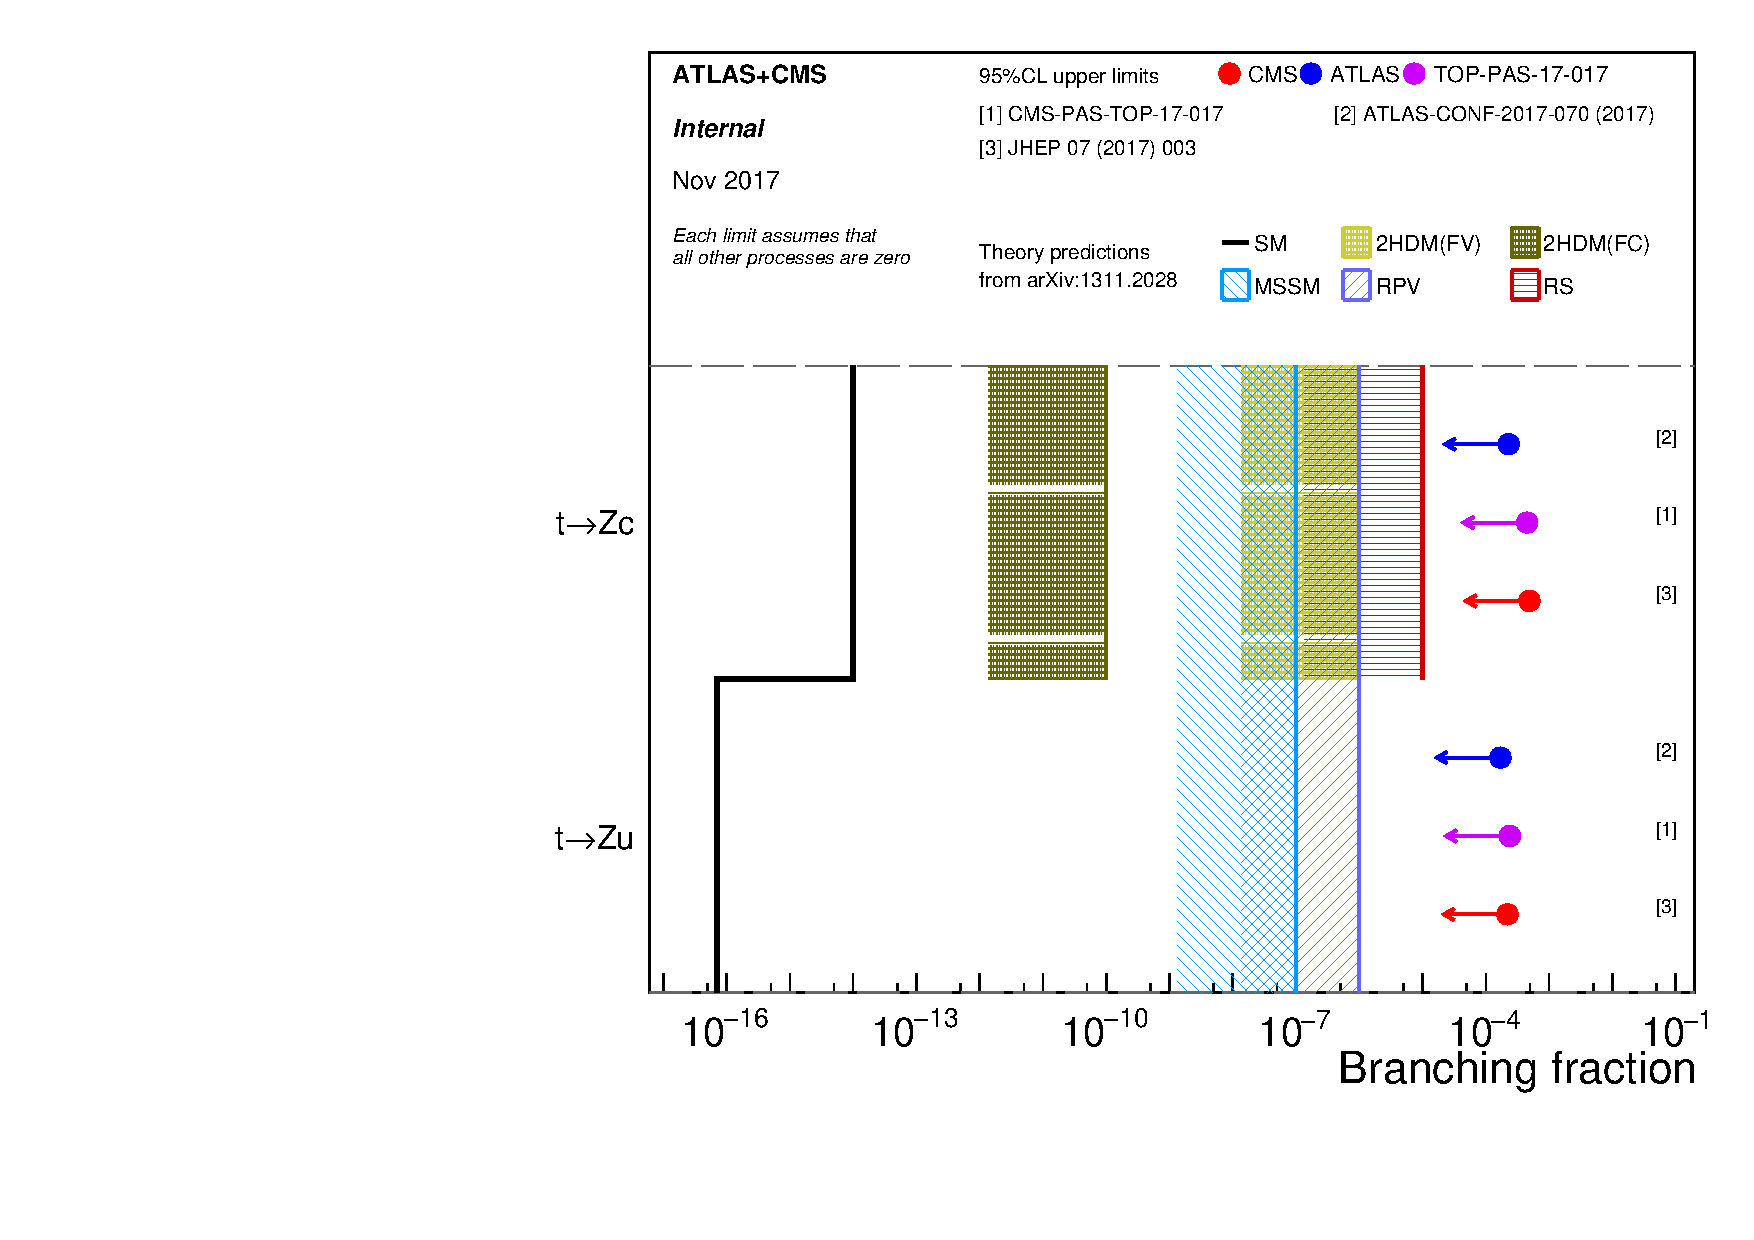
\includegraphics[width=0.49\linewidth]{7_Conclusion/Figures/fcnc_upperlimitszoom.pdf}
	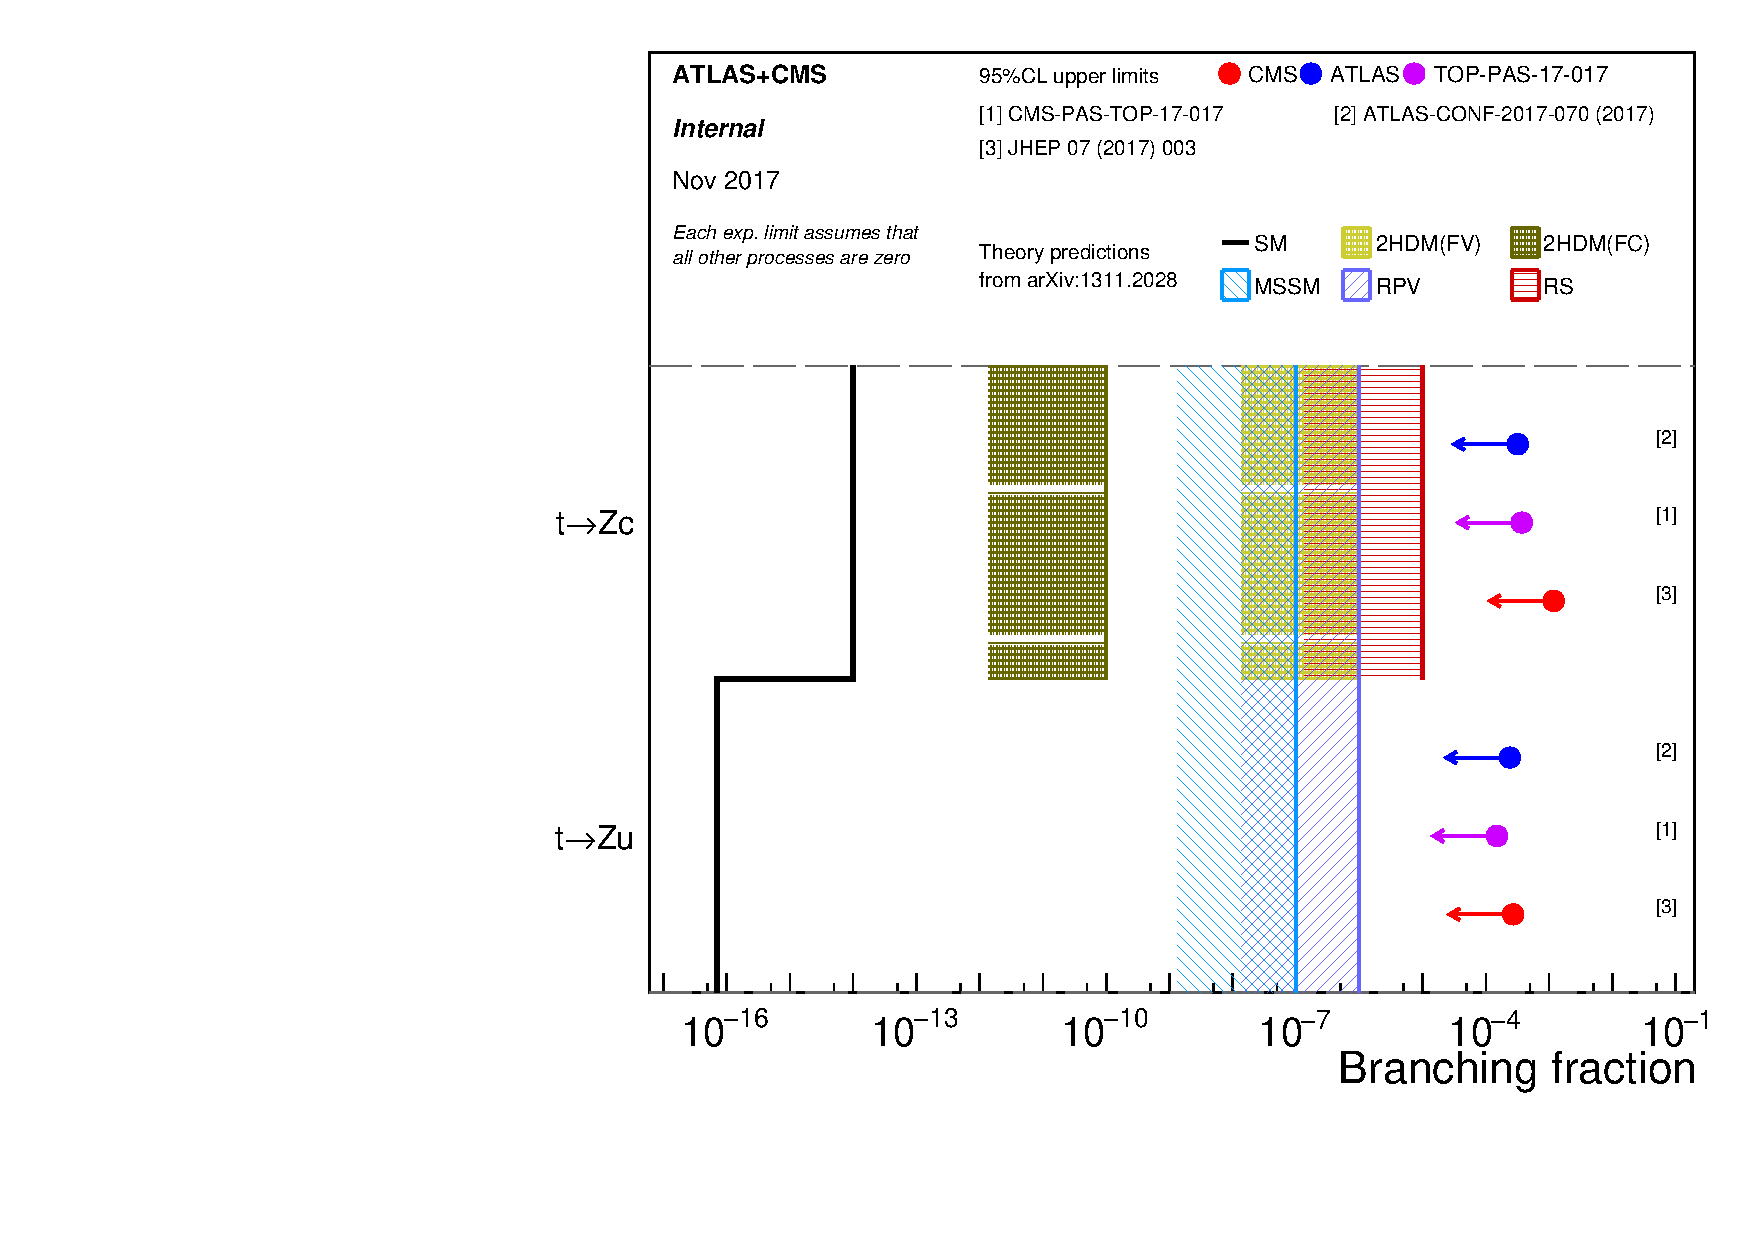
\includegraphics[width=0.49\linewidth]{7_Conclusion/Figures/fcnc_upperlimitszoomexp.pdf}
	\caption{Summary of the most stringent observed (left) and expected (right) upper limits on FCNC \tZq\ at 95\% CL upper limits from CMS (red) and ATLAS (blue) at a centre-of-mass of 8 and 13 \TeV. The results from this thesis are shown in purple. A comparison between theory predictions and experimental limits is shown. Figure adapted from \cite{summarywiki}.}
	\label{fig:zoom}
\end{figure}

Significant improvements are developed with respect to previous searches, namely by using other kinematic variables as input into the BDT as well as a better handle on the \NPL\ background.  The expected limit for the FCNC \Zut\ interaction is more stringent than the expected limit of 2.4$\times 10^{-4}$ for the current  most stringent observedlimit of 1.7$\times 10^{-4}$, set at a centre-of-mass energy of 13~\TeV\ by the ATLAS collaboration~\cite{ATLAS-CONF-2017-070}.  The  observed (expected) limit on the \Zct\ interaction set by ATLAS is 2.3$\times 10^{-4}$ (3.2$\times 10^{-4}$) and its expected limit is comparable with the expected limit presented  in this search.  For the FCNC interactions with a \tZq\ vertex, the branching fractions predicted within the Standard Model or beyond the Standard Model theories are still out of reach. 
%\begin{figure}[htbp]
%	\centering
%	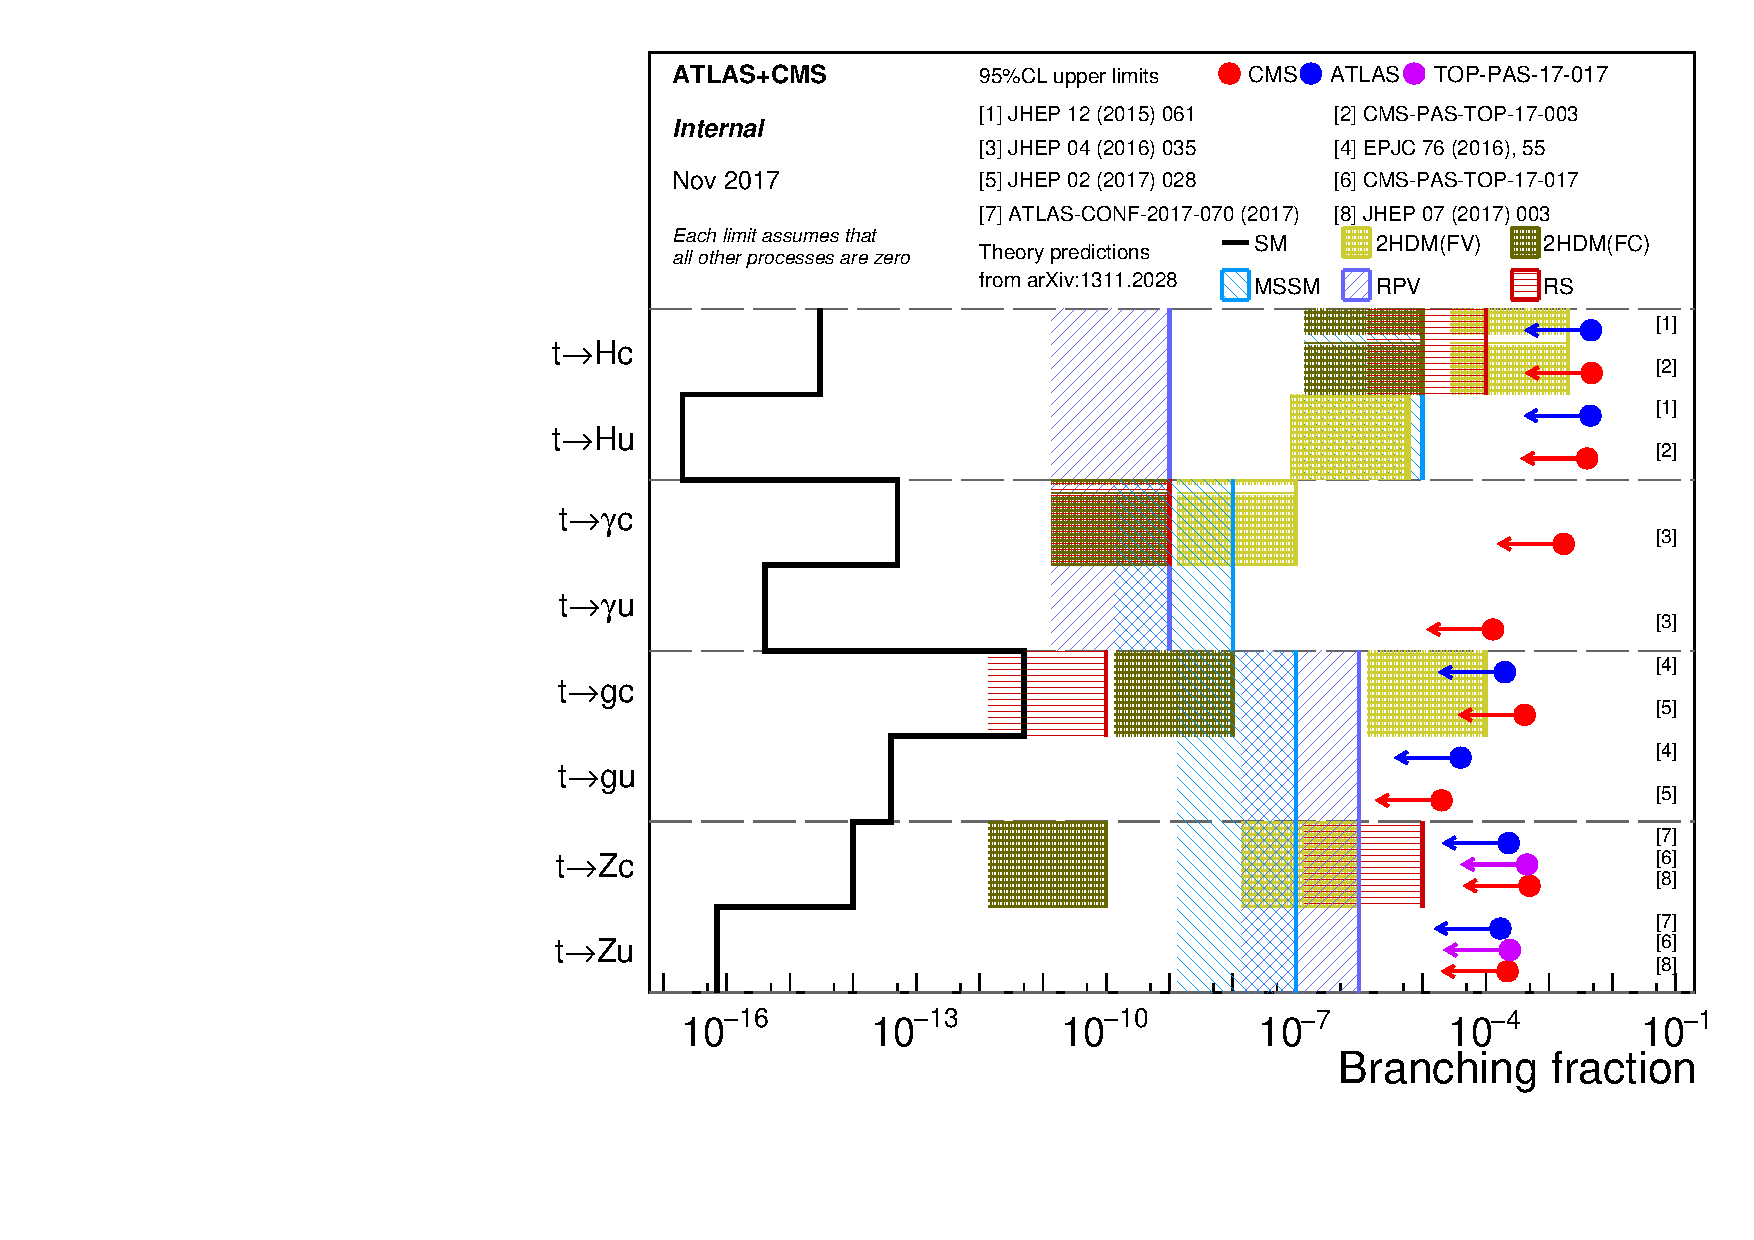
\includegraphics[width=0.7\linewidth]{7_Conclusion/Figures/fcnc_upperlimits.pdf}
%	\caption{Summary of the most stringent upper limits on top-FCNC interactions at 95\% CL upper limits from CMS (red) and ATLAS (blue) at a centre-of-mass of 8 and 13 \TeV. The results from this thesis are shown in purple. A comparison between theory predictions and experimental limits is shown. Figure adapted from \cite{summarywiki}.}
%	\label{fig:fcncupperlimitss}
%\end{figure}



\section{Prospects}
This statistically limited search is expected to have an improved sensitivity when performed on a larger dataset. By extrapolating the current analysis to a dataset of 100~\fbinv\ (full Run~2 dataset), 300~\fbinv\ (Run~2 + Run~3), or 3000~\fbinv\ (HL-LHC), the expected upper limits at 95\% CL are  extracted. %. $\BR(\Ptop \rightarrow \Pup\PZ) < 0.0051\%$ and $\BR(\Ptop \rightarrow \Pcharm\PZ) < 0.014\%$
The templates for the systematic uncertainties are unchanged for the extrapolations. The obtained expected limits at 95\% CL, with respect to the result obtained in the presented search, are shown in \fig{fig:proj}.  The expected limit on the branching fraction is improved with a factor of 3 for the \Zut\ vertex, and and a factor of 4 for the \Zct\ vertex for 100~\fbinv. For 300~\fbinv\ and 3000~\fbinv, the sensitivity is  even more improved and certain beyond the Standard model theories could be confirmed or excluded. Setting statistical limitations aside, the largest systematic uncertainty is coming from the jet energy scale uncertainty. This uncertainty can be decreased by more precise measurements of the jet energy response with more data as well as better methodologies. %A  calorimeter could help reducing the uncertainty.  % ook better handle op pu sinds hiervoor gecorrigeerd wordt
\begin{figure}
	\centering
	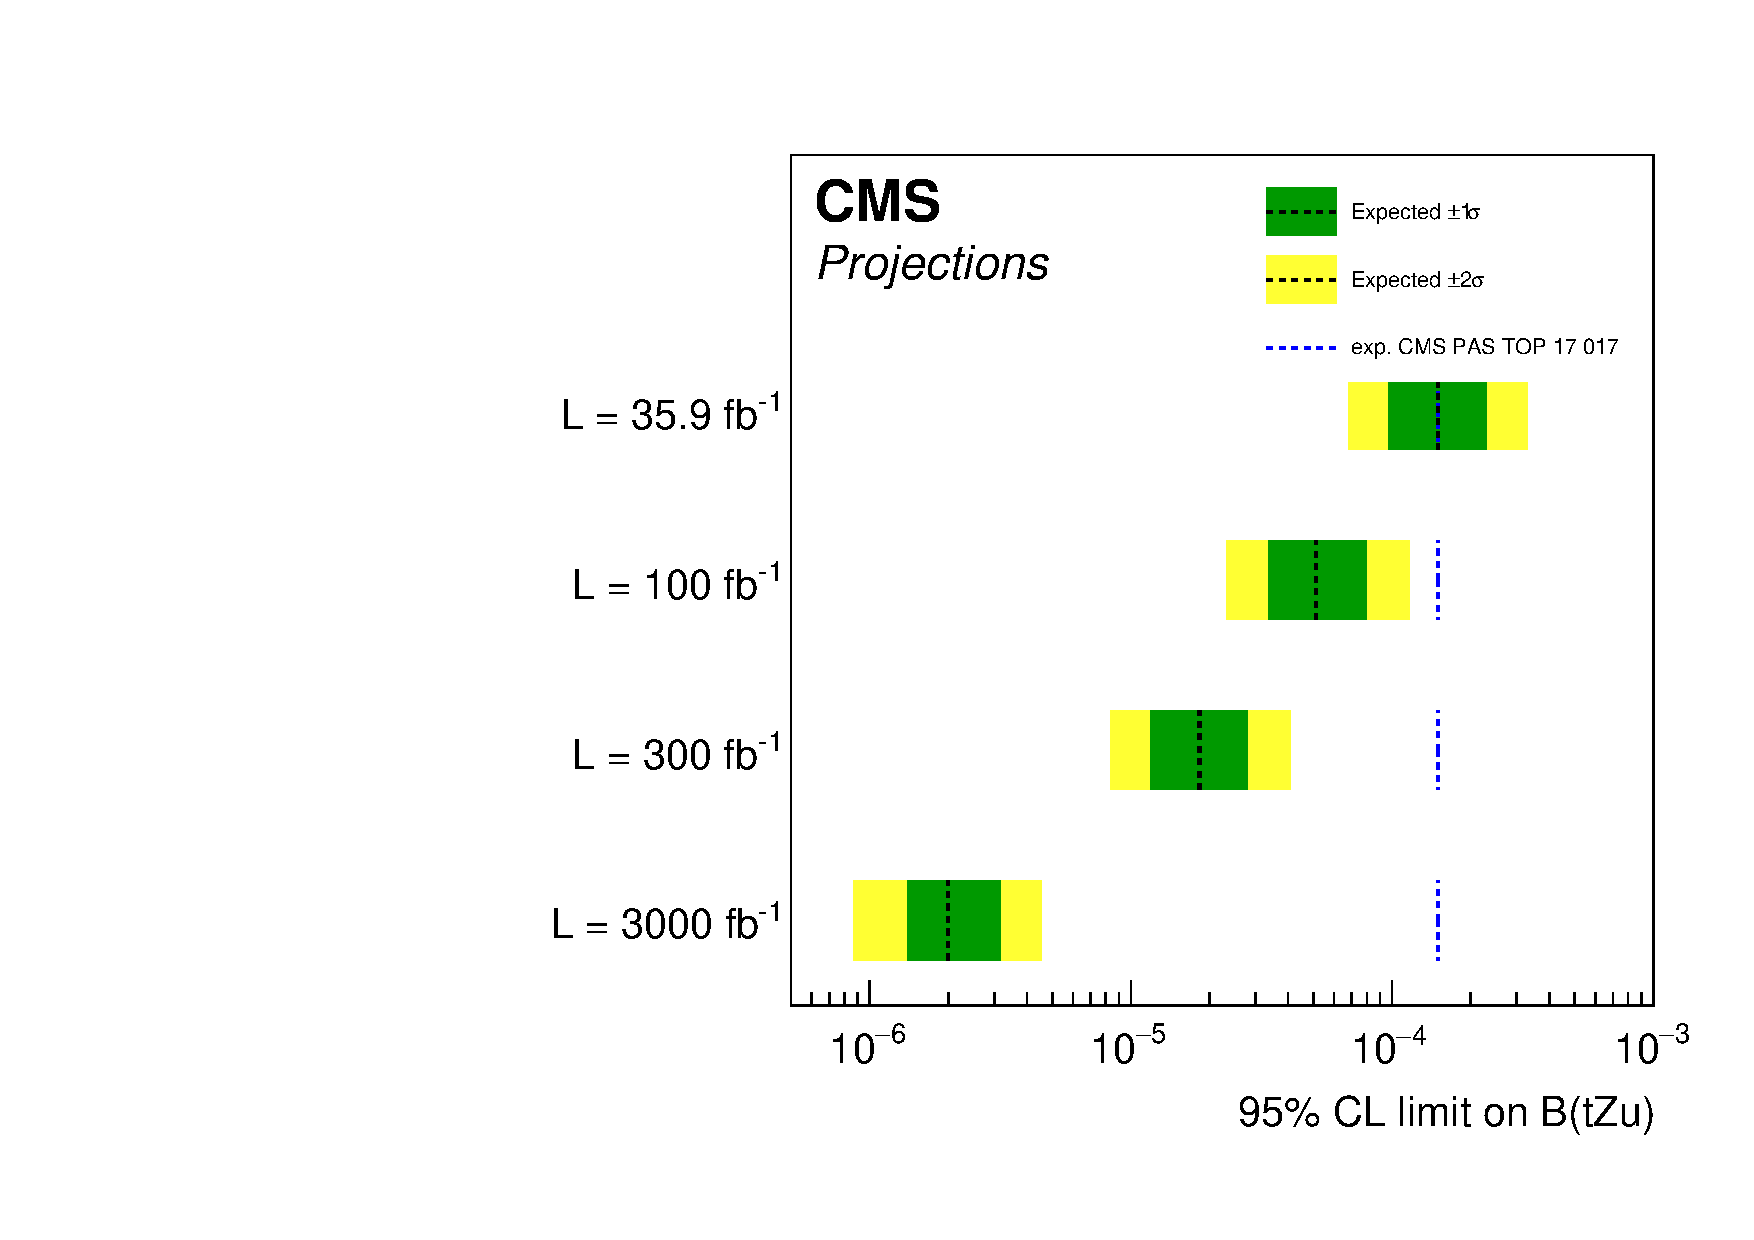
\includegraphics[width=0.49\linewidth]{7_Conclusion/Figures/TOP-17-017_limitsZutProj.pdf}
	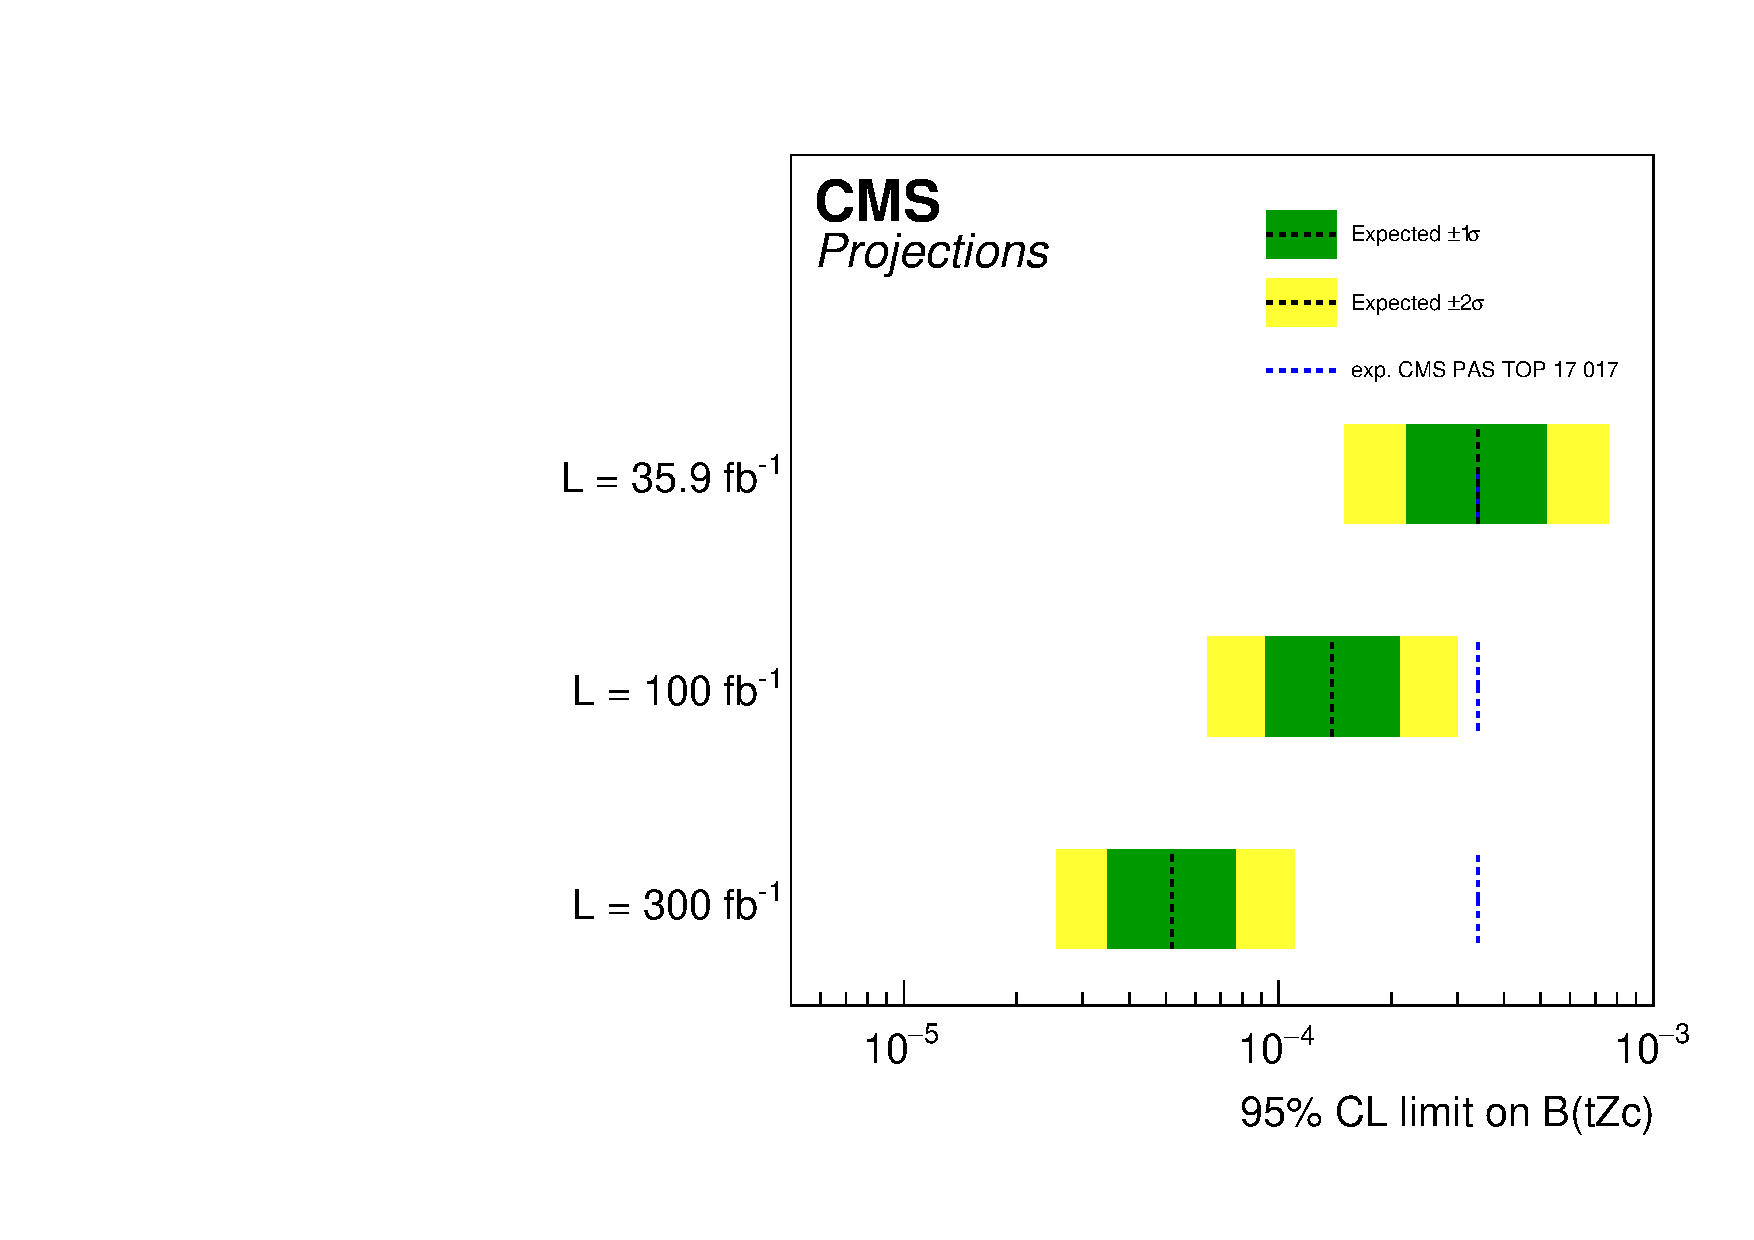
\includegraphics[width=0.49\linewidth]{7_Conclusion/Figures/TOP-17-017_limitsZctproj.pdf}
	\caption{The expected limit at 95\% CL for the \Zut\ (left) and \Zct\ interaction for an integrated luminosity of 100; 300, and 3000 \fbinv, extrapolated from the result obtained in this thesis, indicated with the blue (dashed) lines. }
	\label{fig:proj} % /user/ivanpari/CMSSW_8_0_26_patch1/src/TopBrussels/FCNCAnalysis > python limitsprj.py 
\end{figure}


A new pixel detector was installed in March 2017 and is expected to enhance the performance of heavy-flavour tagging which should help improve the sensitivity of the analysis. Furthermore, the recently developed charm tagging algorithm~\cite{CMS-PAS-BTV-16-001} could help the sensitivity of the analysis.  Especially  the sensitivity for the top quark pair FCNC signal involving a \Zct\ vertex could benefit from this algorithm. Here, some exemplary distributions related to charm tagging are shown for a selection of exactly three leptons for which a lepton pair is compatible with the Z boson, and at least one jet. At CMS, a collection of c-tagged jets can be created in a similar way as is done for b-tagged jets. Dedicated discriminants are created from multivariate analyses aiming for a discrimination of charm quark jets against light-flavour jets (CvsL),  and charm quark jets against bottom quark jets (CvsB). By placing thresholds on both discriminators at the same time, the collection of c-tagged jets is created for different working points. The distribution of the charm jet multiplicities according to the different working points are shown in \fig{fig:charm}. The loose working point is defined to keep 90\% of the charm quark jets, and only 45\% of the bottom quark jets, whilst keeping 99\% of the light-flavour jets. The tight working point is defined for discriminating charm quark jets from light-flavour jets and keeps 20\% of the charm quark jets, while 0.02\% of the light-flavour jets are selected. For this working point, also 24\% of the bottom quark jets are surviving. The medium working point creates an intermediate state where 39\% of the charm quark jets are kept, with 26\% of the bottom quark jets, and 19\% of the light-flavour jets. One can see that the distribution of the charm quark jet multiplicity according to the tight working point shows the most promising result. Here, there is one c-tagged jet expected for the top quark pair FCNC signal via the \Zct\ interaction, while less events are entering the one c-tagged jet region for the  background processes.
\begin{figure}[htbp]
	\centering
	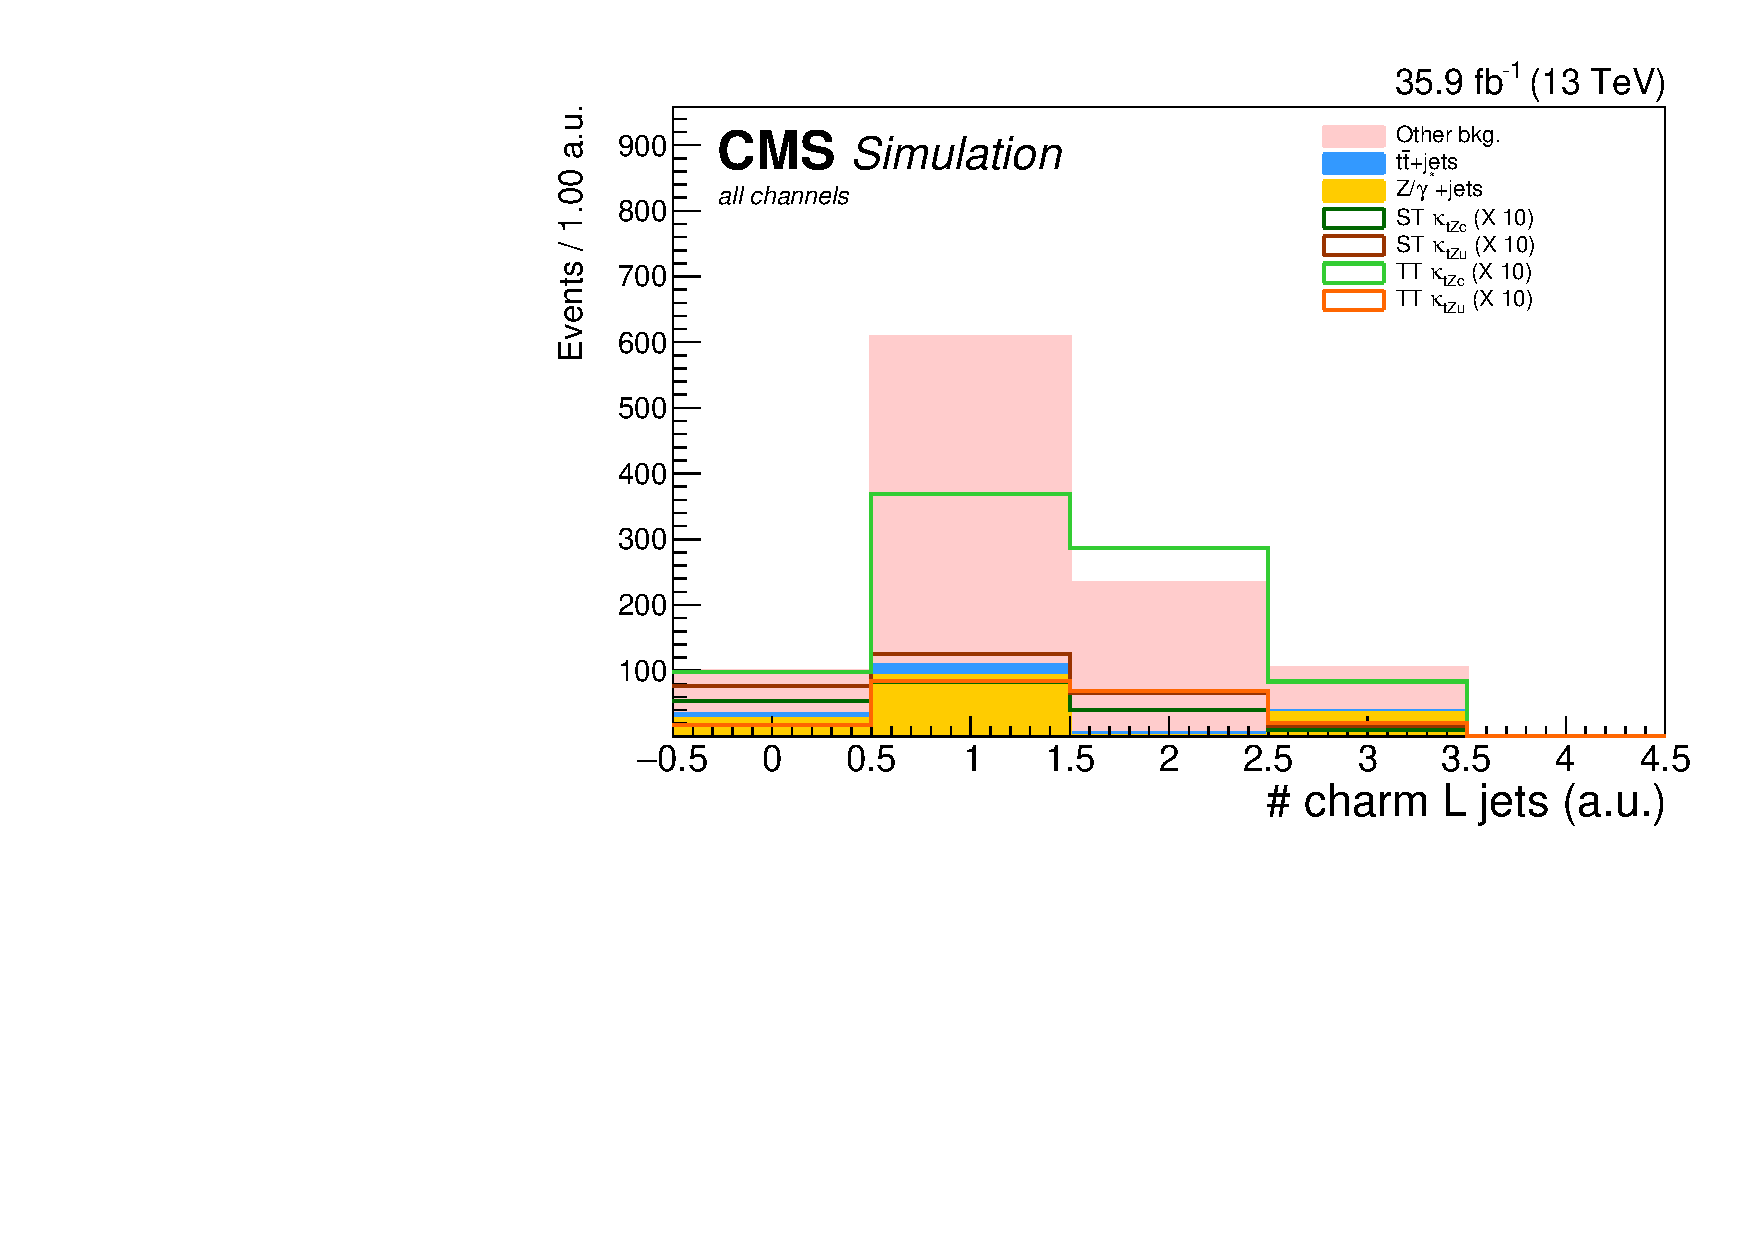
\includegraphics[width=0.49\linewidth]{7_Conclusion/Figures/charmtagging/3lepcontrol_dilep_nJetsCharmL_all_Stack}
	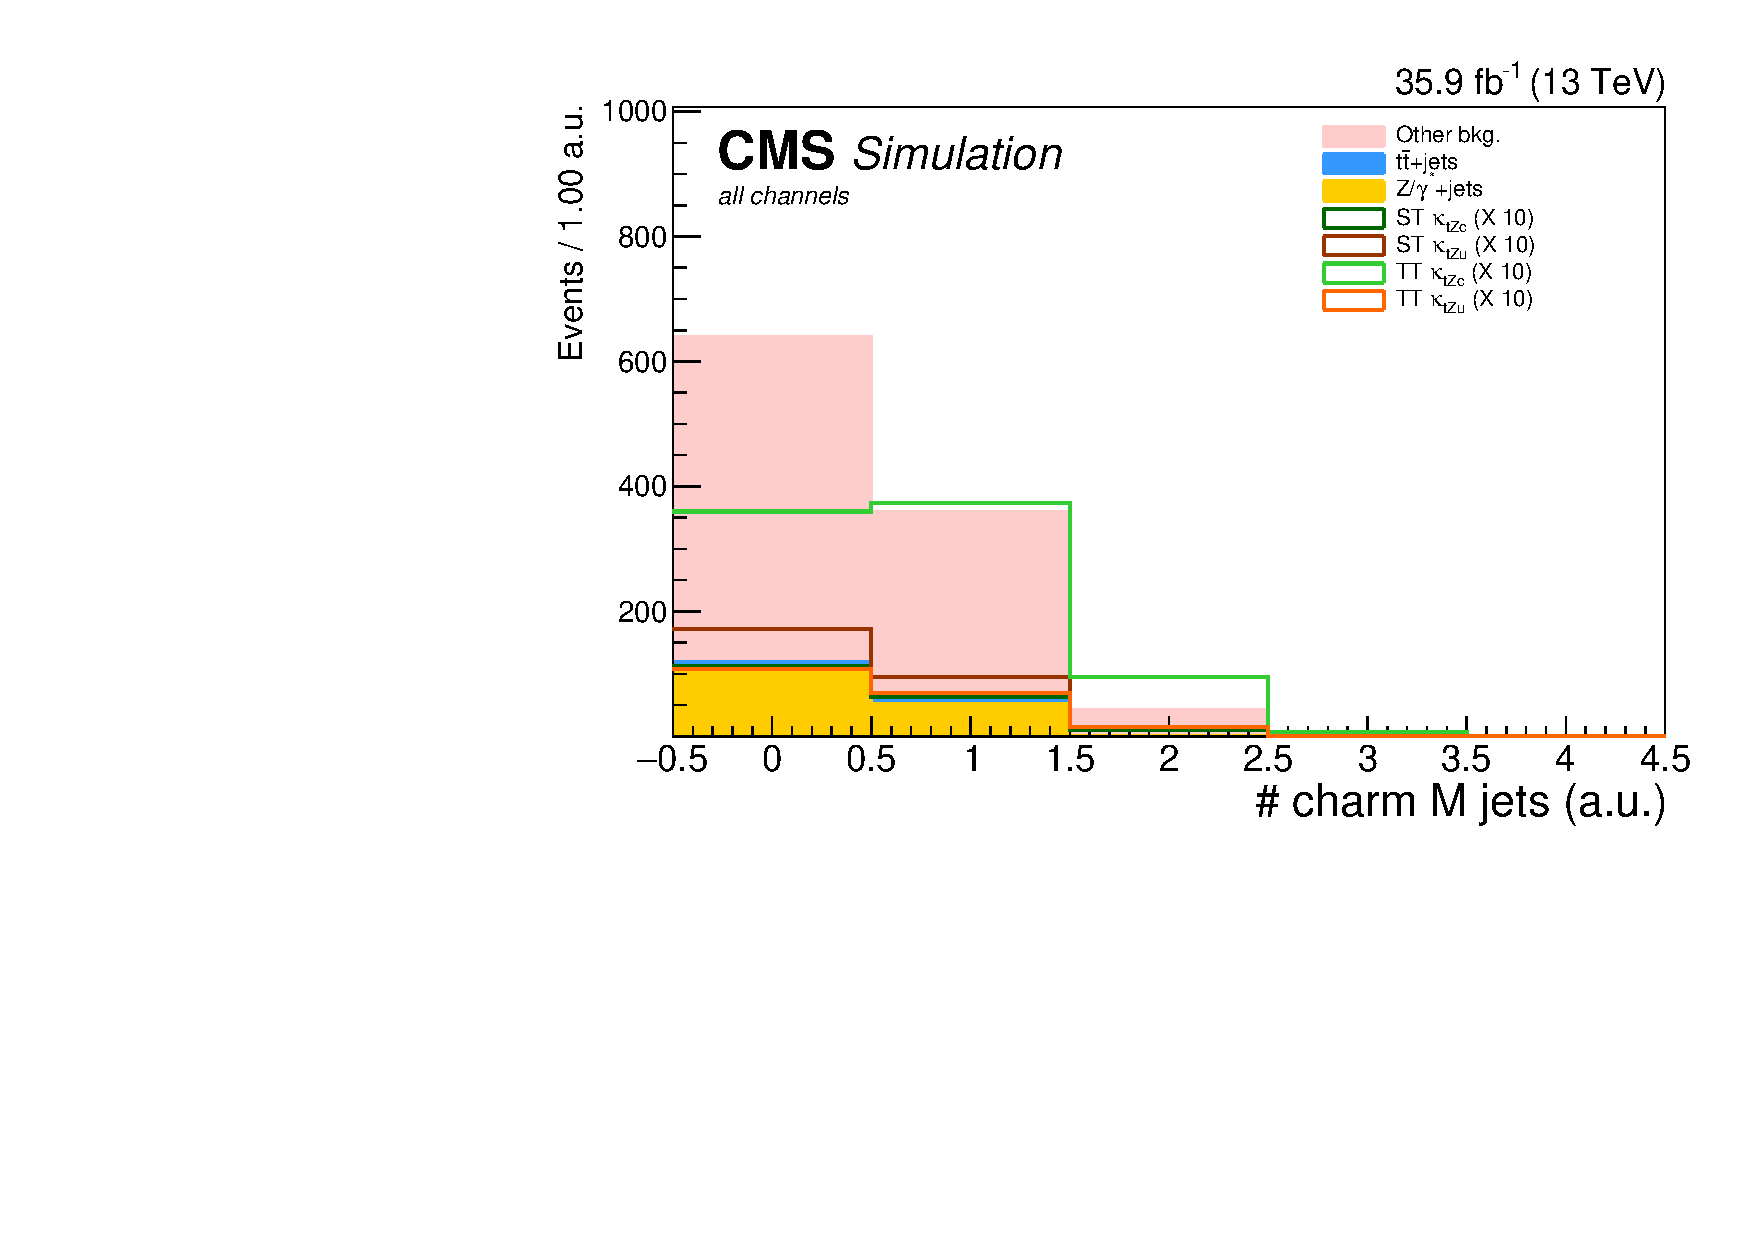
\includegraphics[width=0.49\linewidth]{7_Conclusion/Figures/charmtagging/3lepcontrol_dilep_nJetsCharmM_all_Stack}
	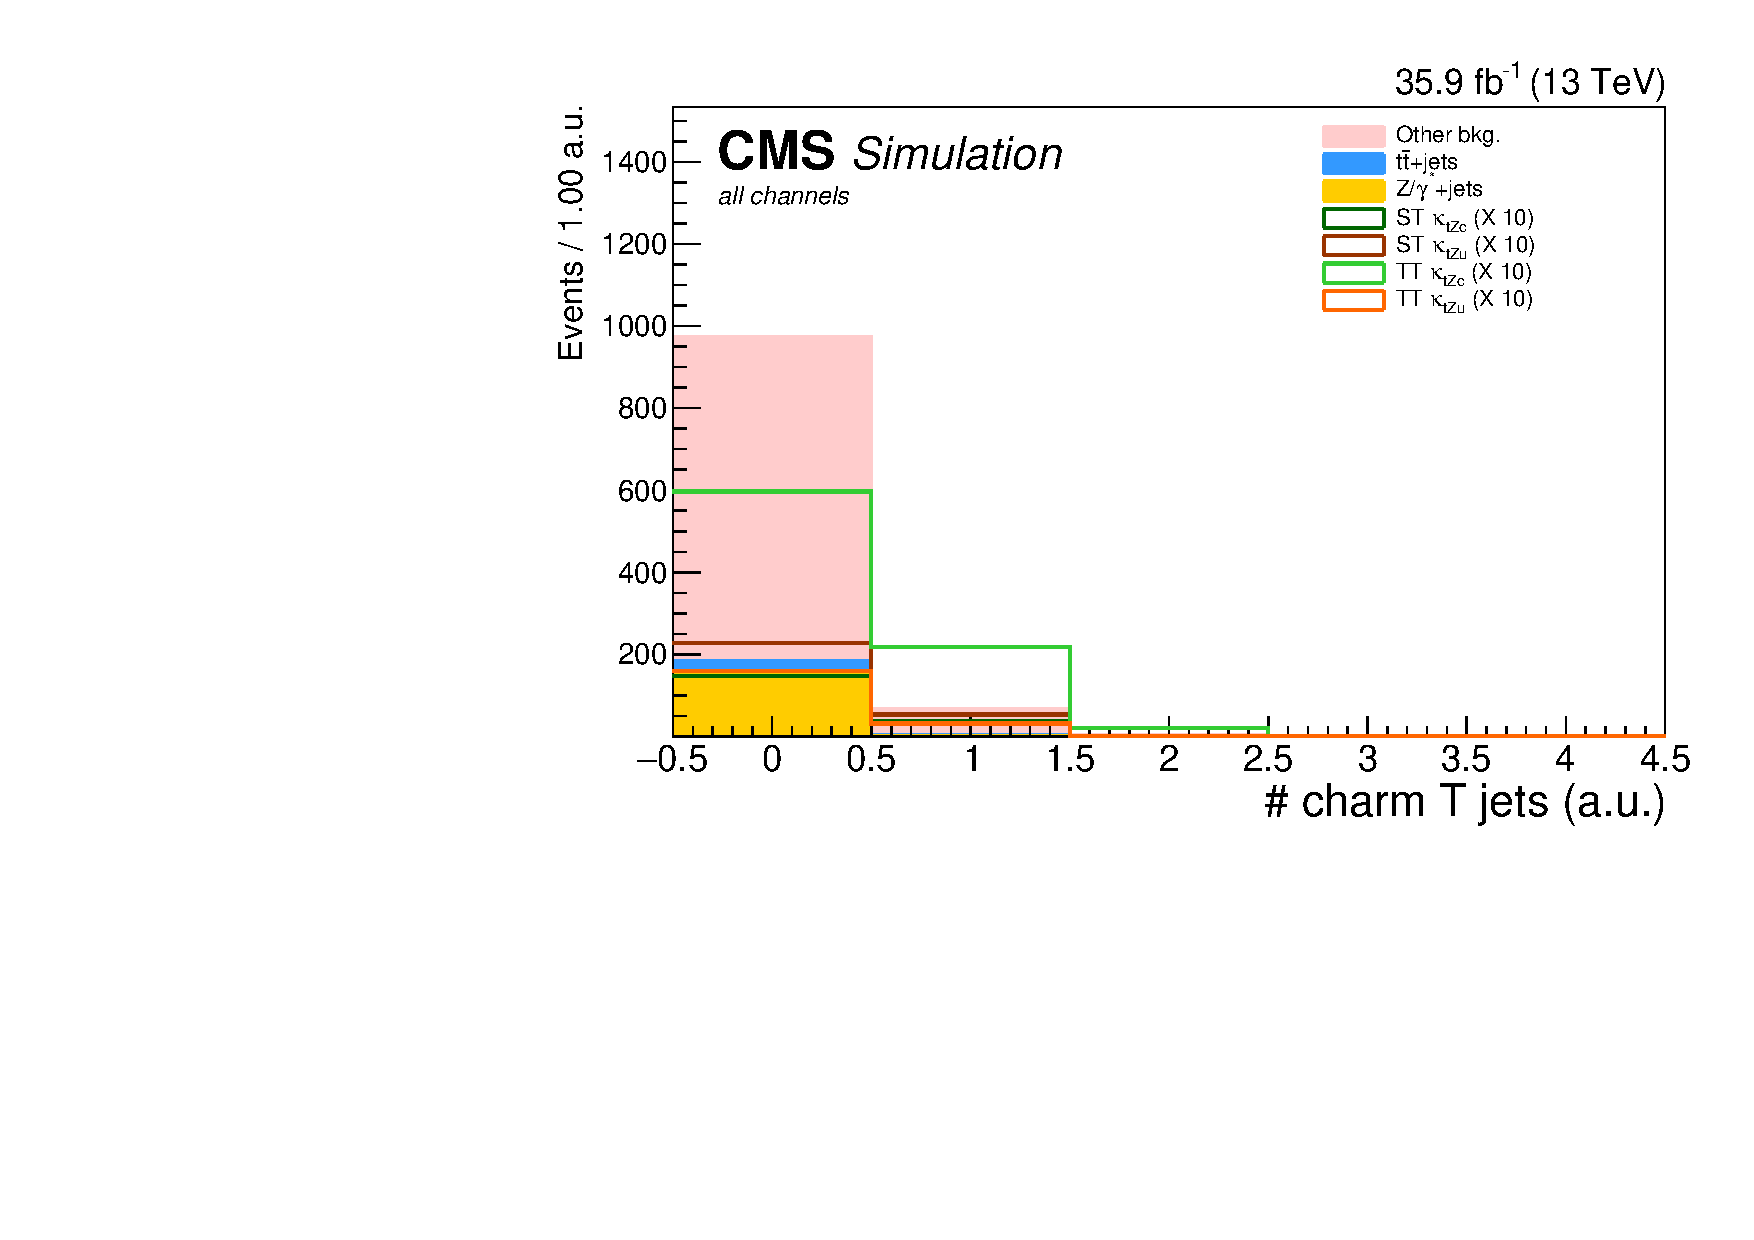
\includegraphics[width=0.49\linewidth]{7_Conclusion/Figures/charmtagging/3lepcontrol_dilep_nJetsCharmT_all_Stack}
	\caption{Distributions of the charm jet multiplicities according to different working points: loose (L), medium (M), and  tight (T). After a three-lepton, for which a lepton pair is compatible with the Z boson, selection with jets.}
	\label{fig:charm}
\end{figure}
\begin{figure}[htbp]
	\centering
	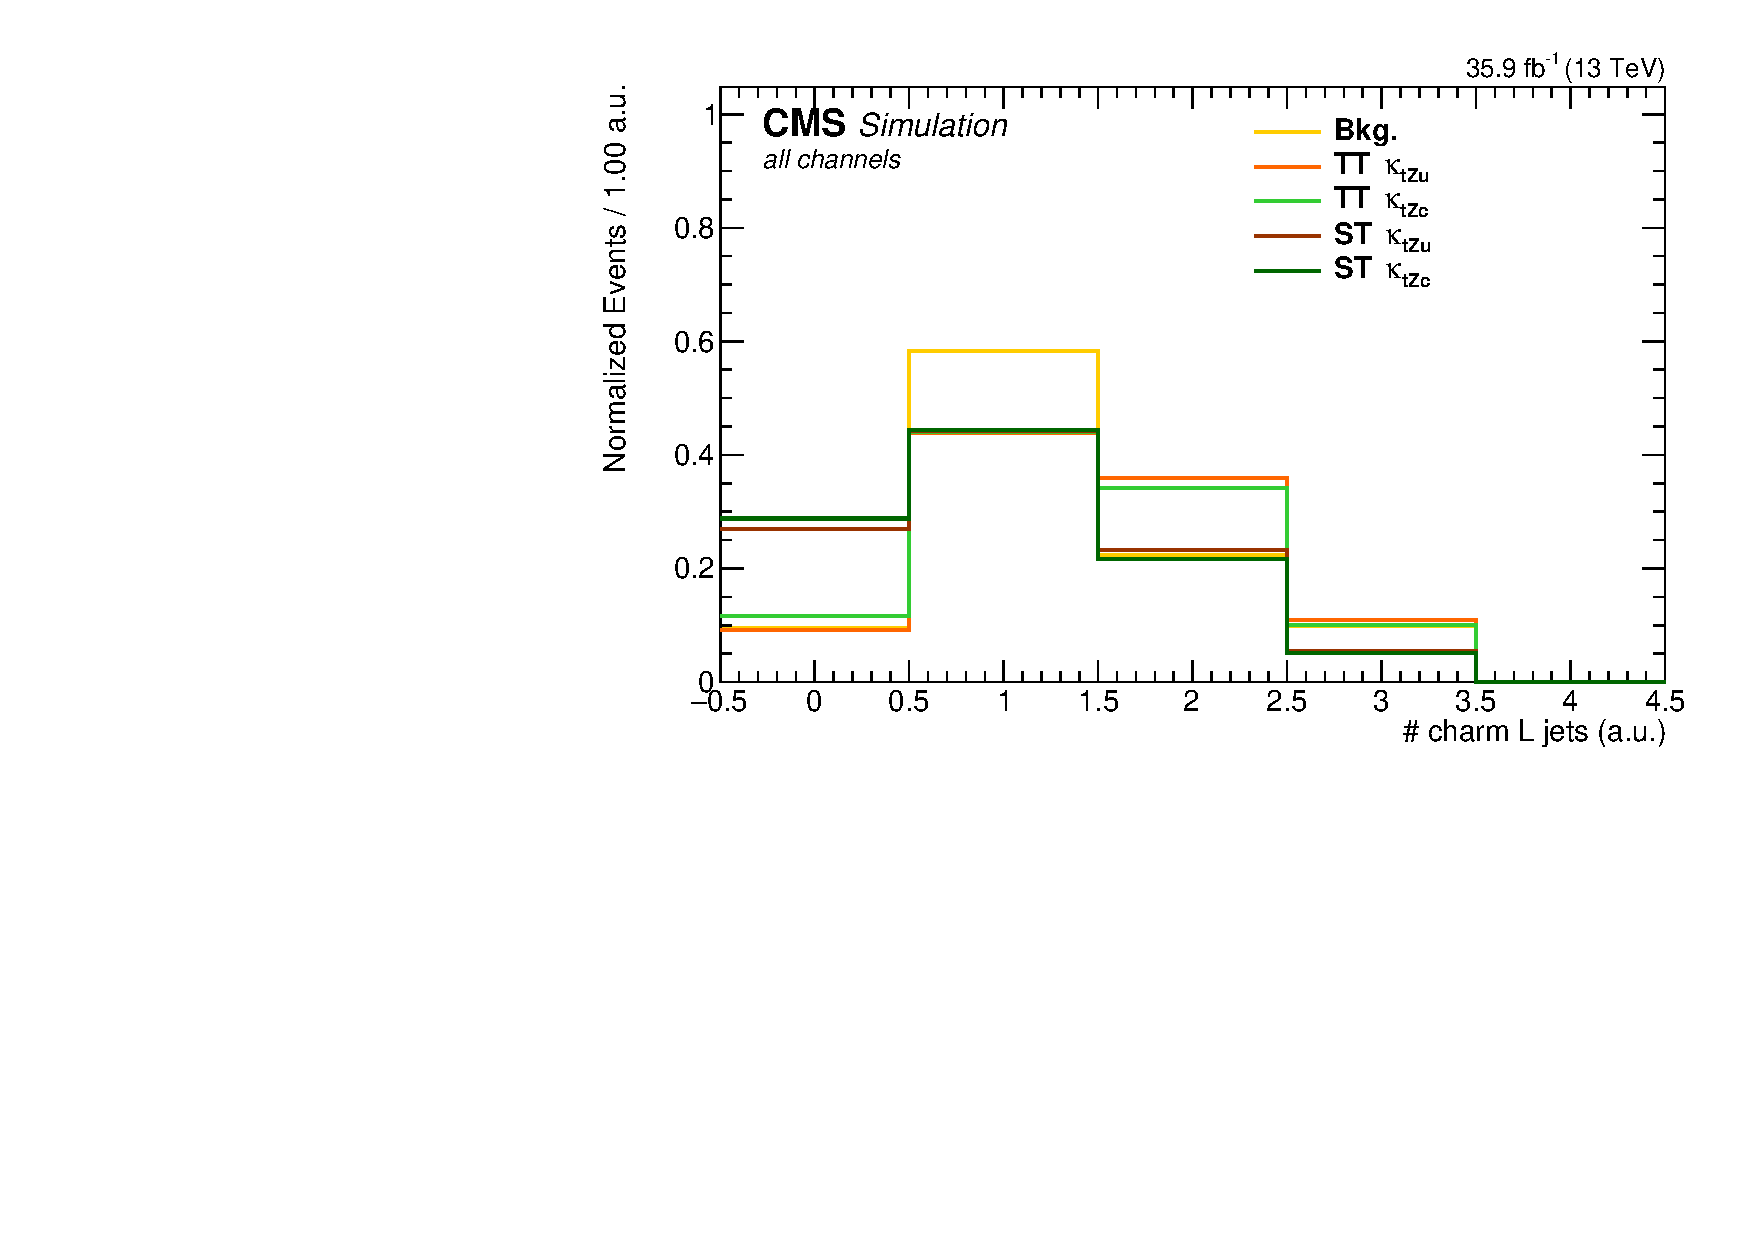
\includegraphics[width=0.49\linewidth]{7_Conclusion/Figures/charmtagging/3lepcontrol_dilep_nJetsCharmL_all_Normalized}
	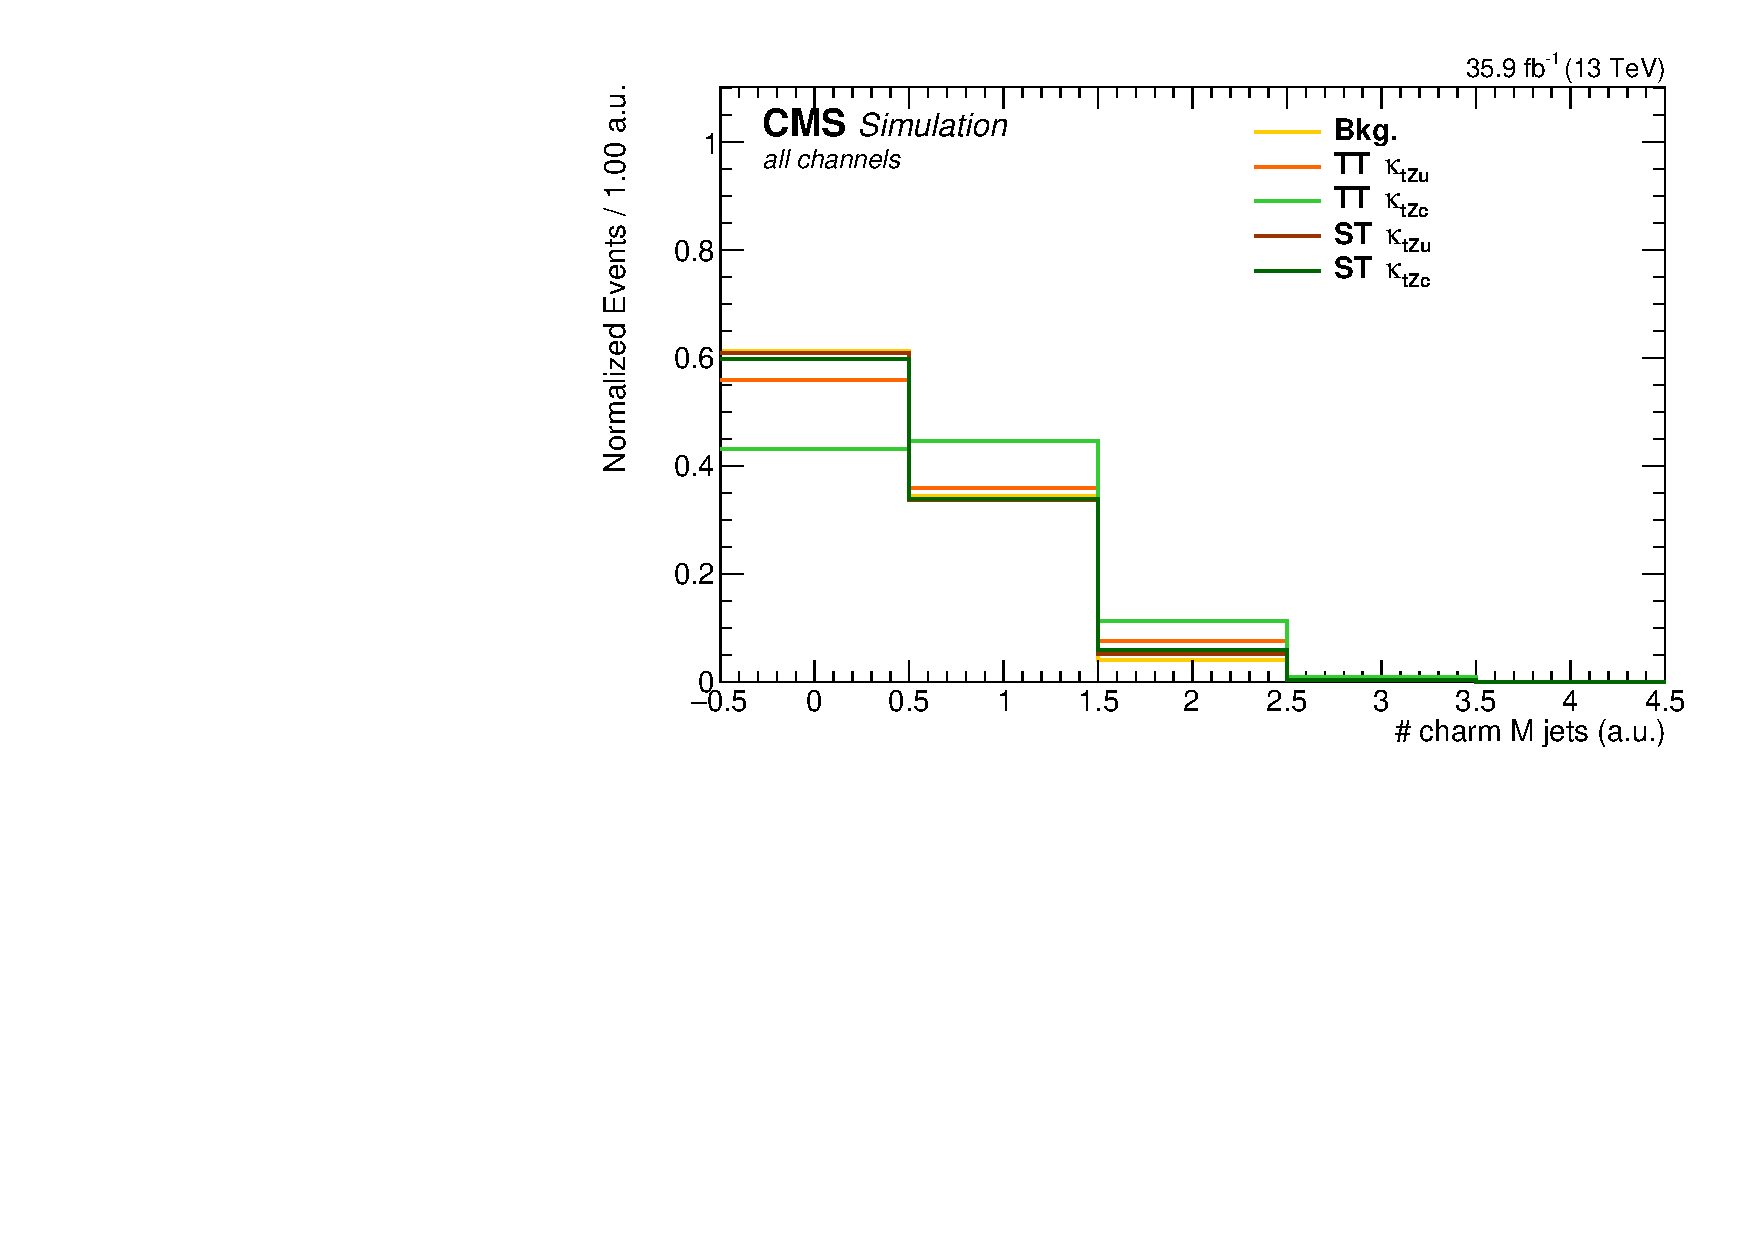
\includegraphics[width=0.49\linewidth]{7_Conclusion/Figures/charmtagging/3lepcontrol_dilep_nJetsCharmM_all_Normalized}
	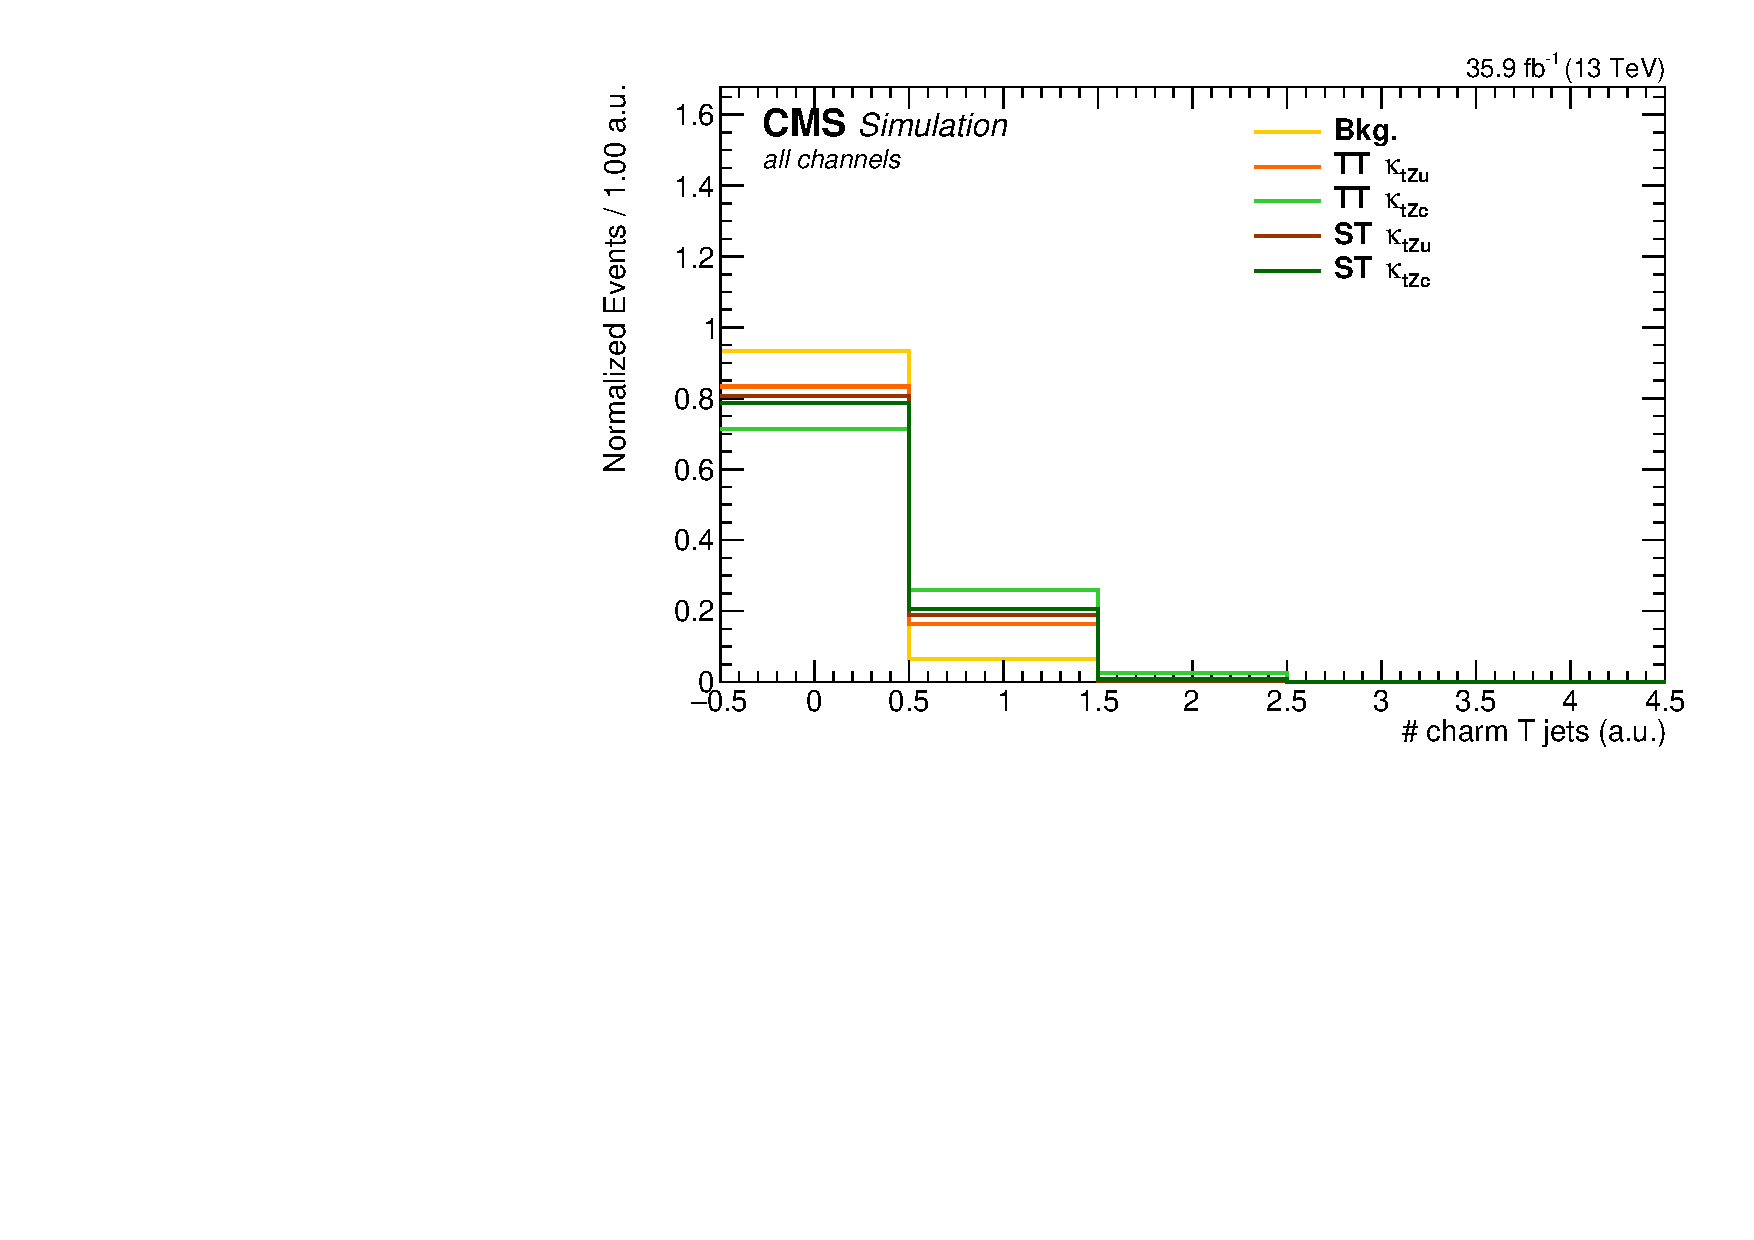
\includegraphics[width=0.49\linewidth]{7_Conclusion/Figures/charmtagging/3lepcontrol_dilep_nJetsCharmT_all_Normalized}
	\caption{Distributions of the charm jet multiplicities according to different working points: loose (L), medium (M), and  tight (T). After a three-lepton, for which a lepton pair is compatible with the Z boson, selection with jets.}
	\label{fig:charem}
\end{figure}


 The distributions related to the shape of the CvsB and CvsL discriminants are shown in \fig{fig:ctagging}. The CvsB discriminant of the jet with the (2nd) highest-\pt\ in the event is dominated by the top quark pair FCNC signal, for the \kZct\ coupling, for the lower values. A similar behaviour is found when one looks at the CvsB discriminator of all jets in the event. For the CvsL discriminant, the FCNC signal is peaking at one, while the  distribution of the background processes peaks at -0.4 and declines towards higher discriminant values. This behaviour is visible for the distributions of the CvsL discriminant of the (2nd) highest-\pt\ in the event, as well as the CvsL discriminant values of all the jets in the event. One can even exploit this behaviour even more by looking at the distribution for CvsL discriminator for the jet with the highest CvsL discriminator value. For the CvsB discriminator, this is  done by looking at the jet with the lowest  CvsB discriminator value.
\begin{figure}[htbp]  % OutputPlots/171128_1746
	\centering
	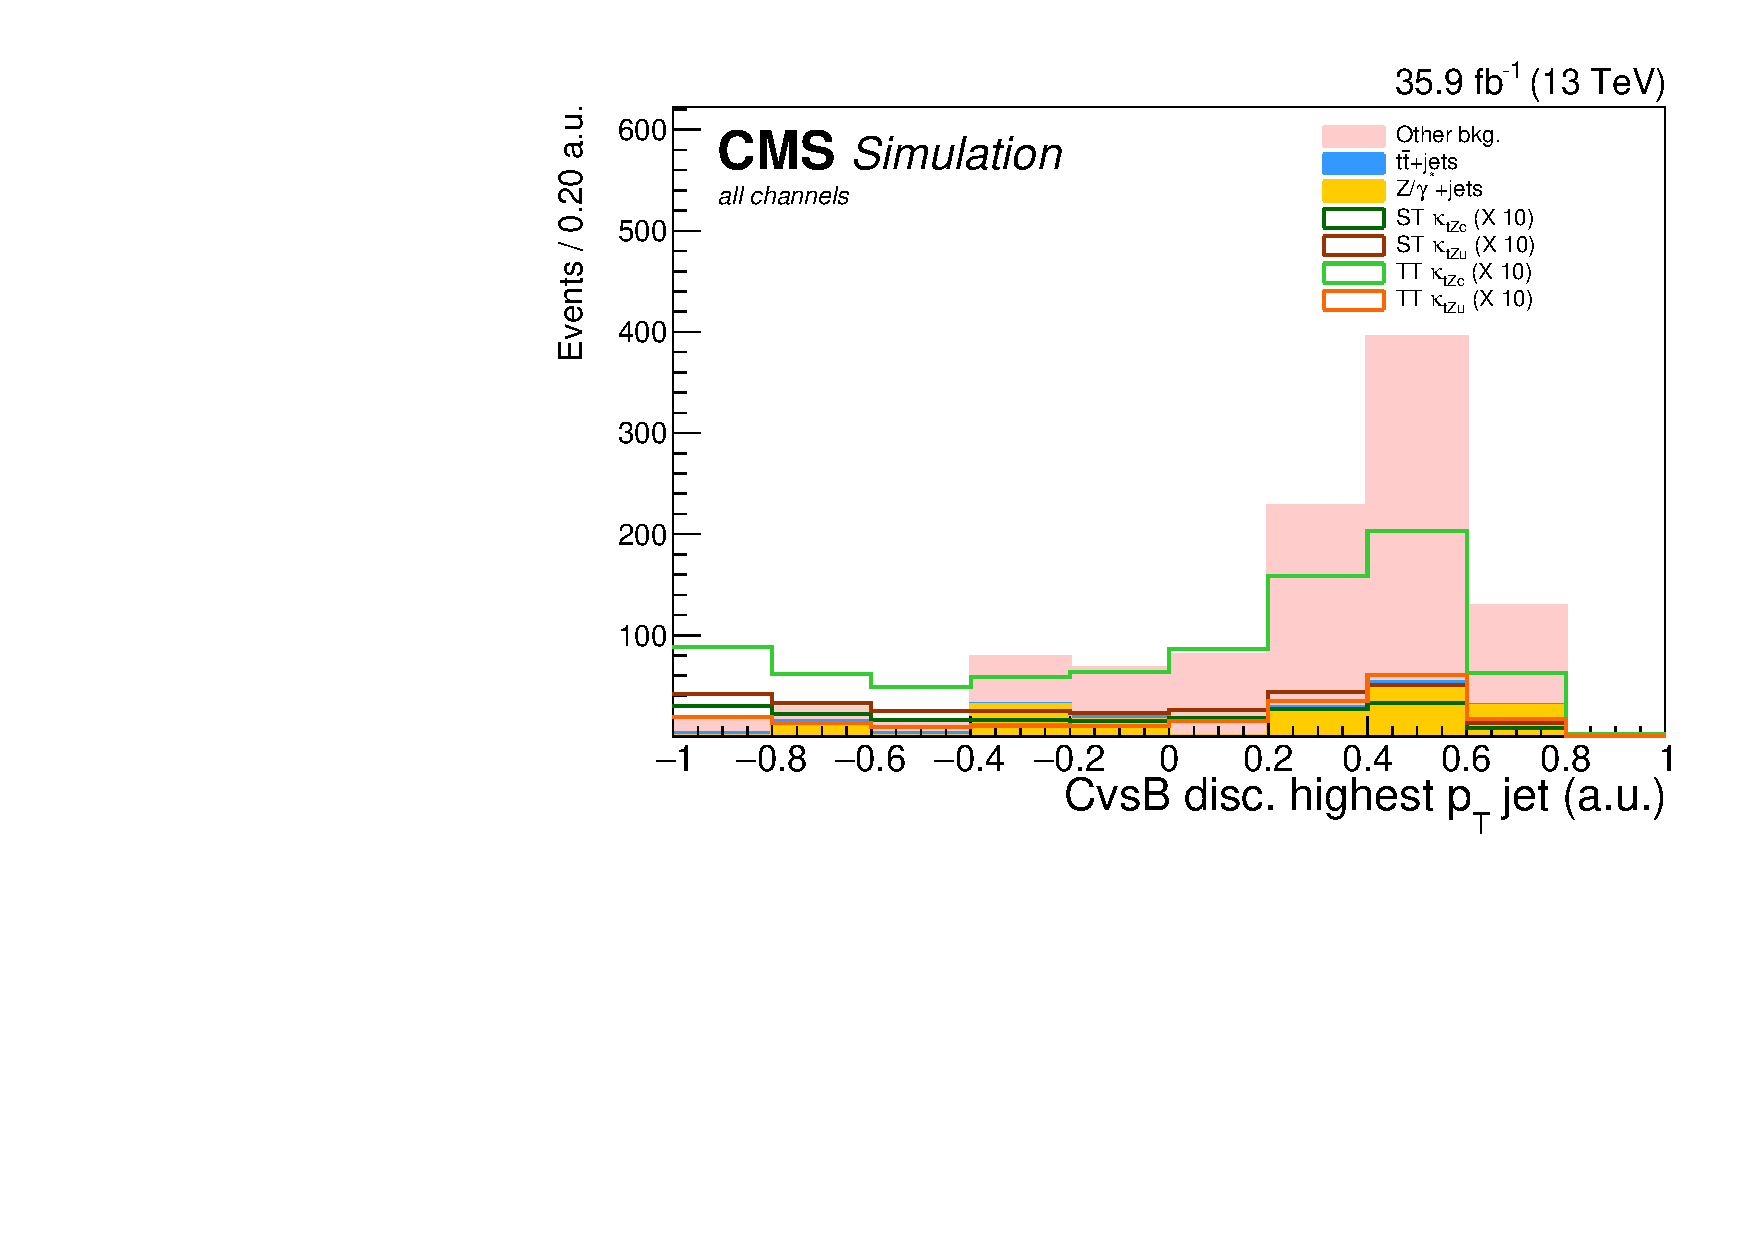
\includegraphics[width=0.49\linewidth]{7_Conclusion/Figures/charmtagging/3lepcontrol_dilep_CvsBdisc_0jet_all_Stack}
		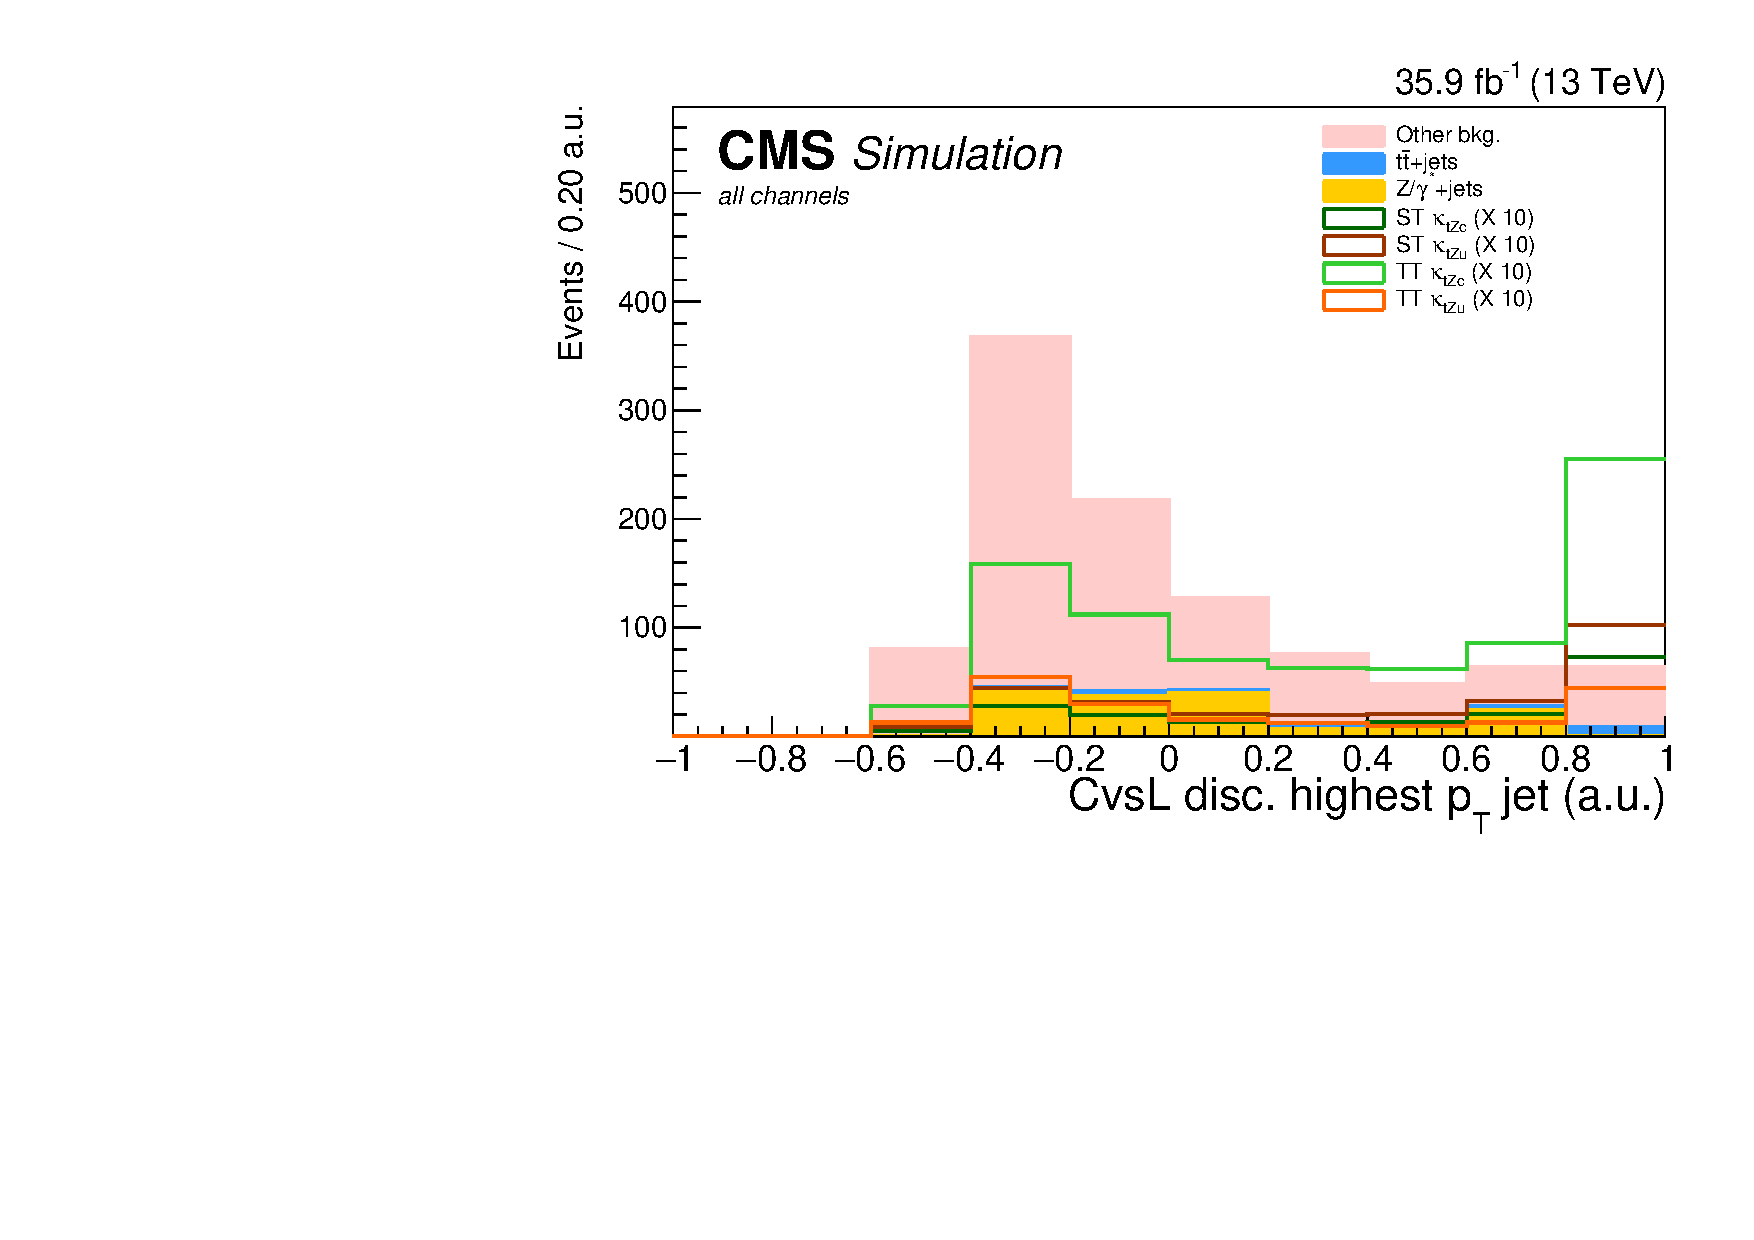
\includegraphics[width=0.49\linewidth]{7_Conclusion/Figures/charmtagging/3lepcontrol_dilep_CvsLdisc_0jet_all_Stack}
	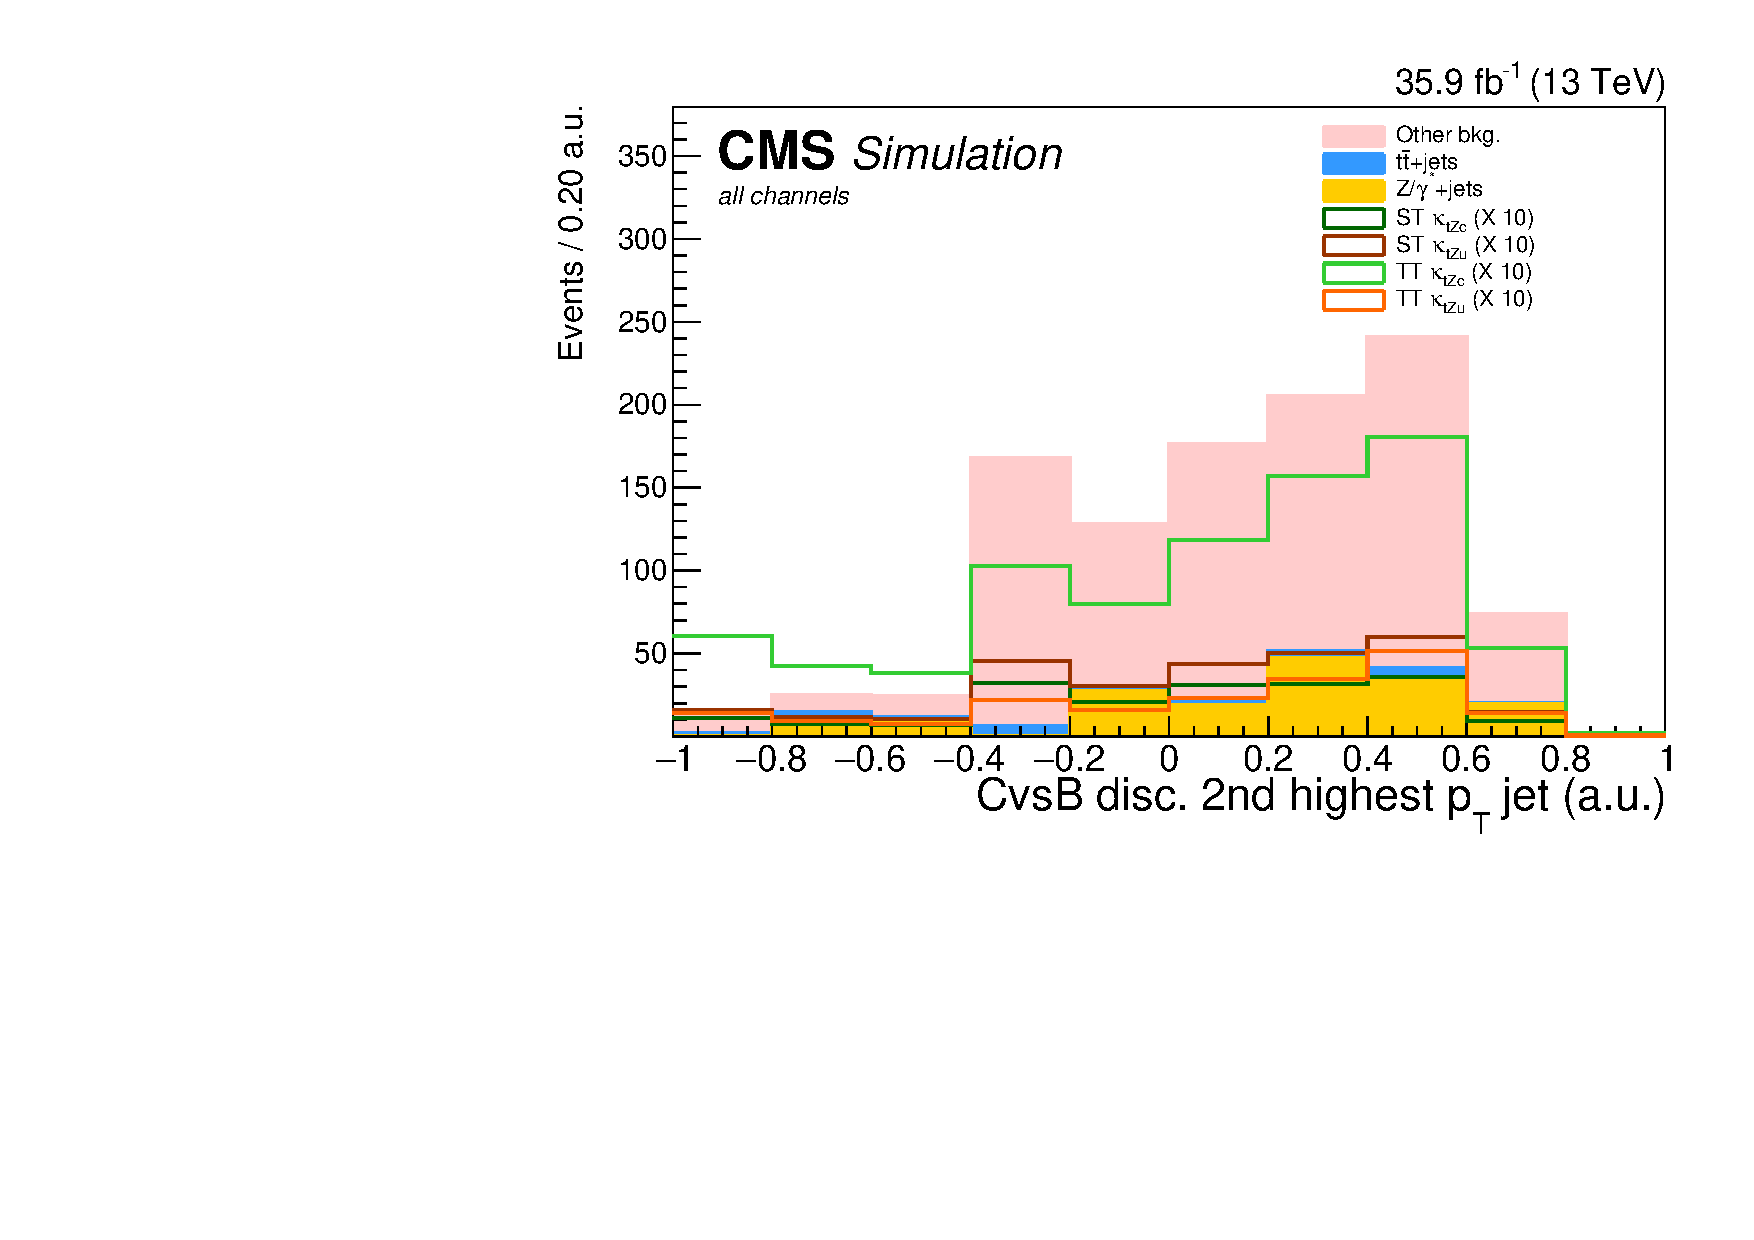
\includegraphics[width=0.49\linewidth]{7_Conclusion/Figures/charmtagging/3lepcontrol_dilep_CvsBdisc_1jet_all_Stack}
		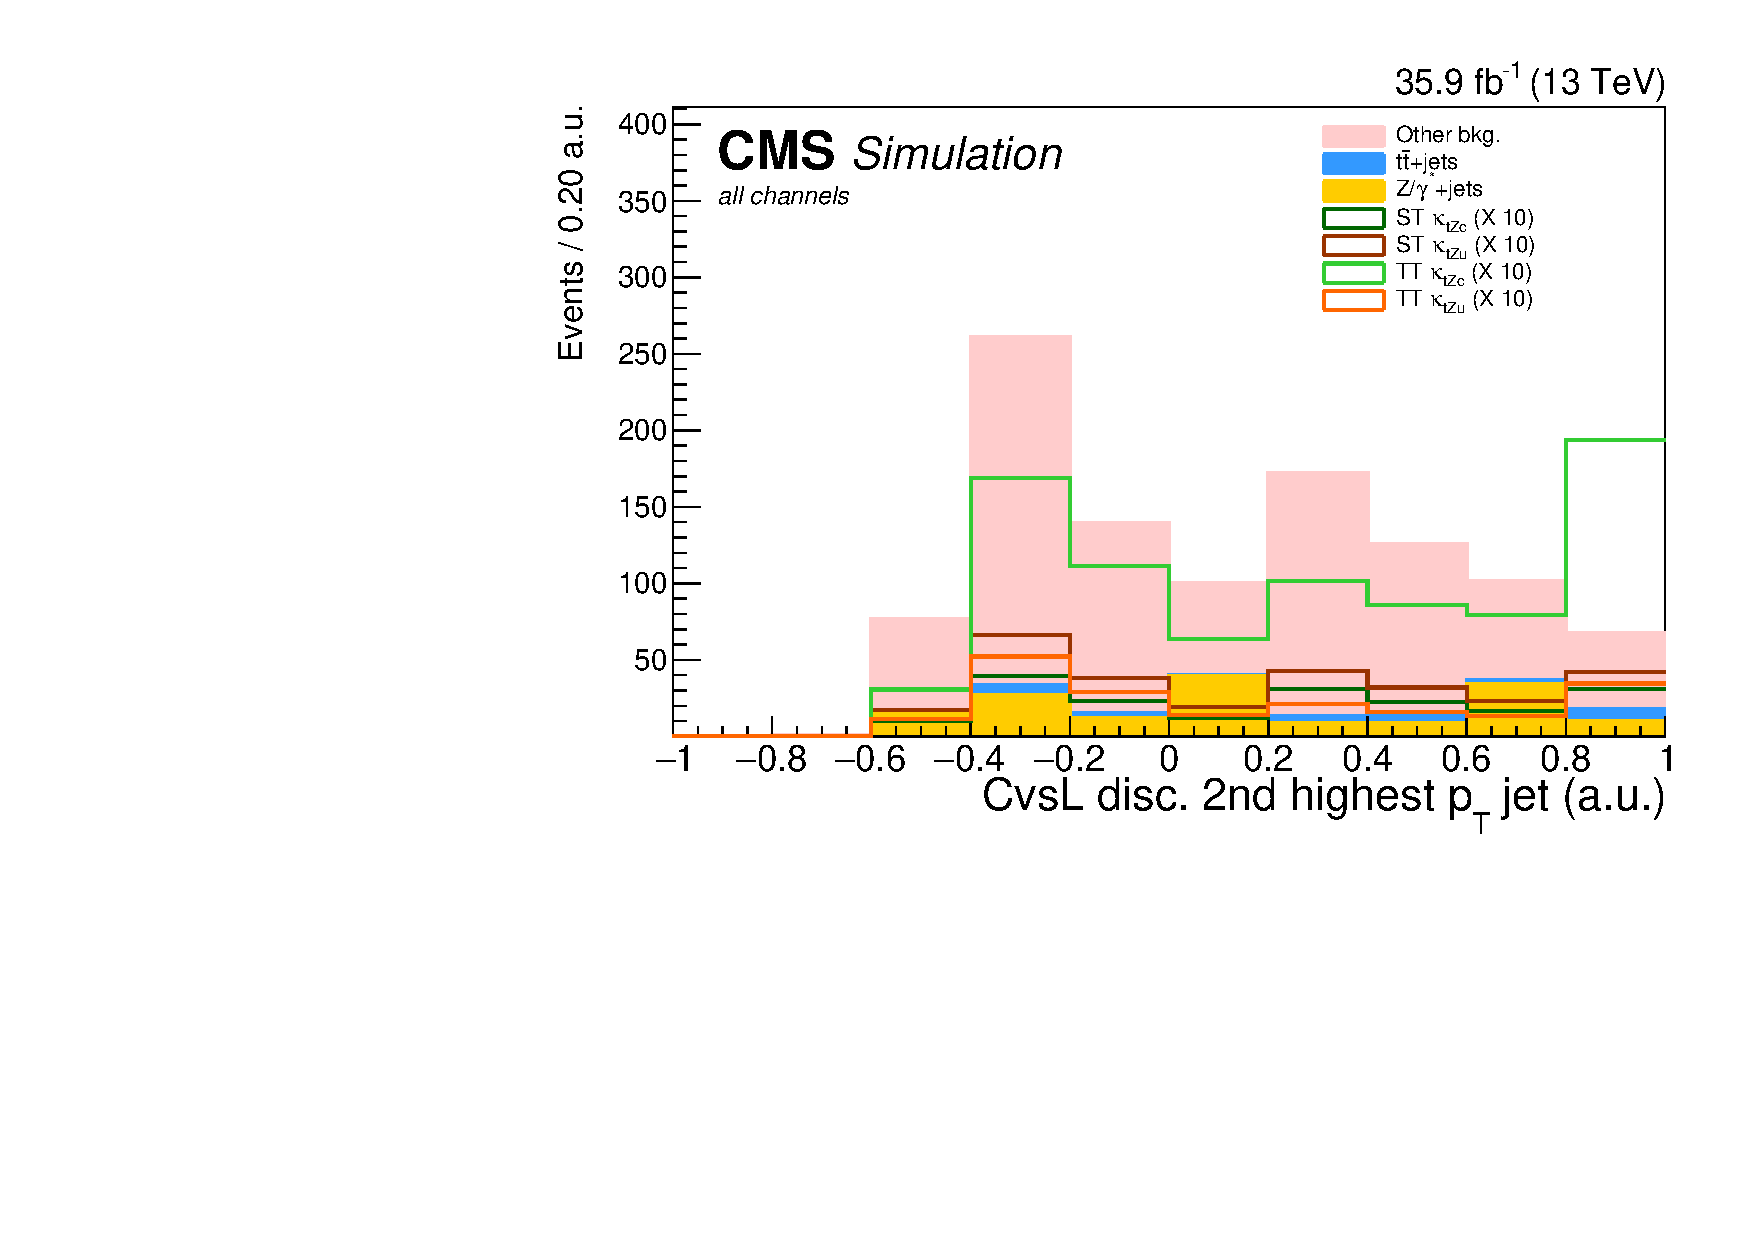
\includegraphics[width=0.49\linewidth]{7_Conclusion/Figures/charmtagging/3lepcontrol_dilep_CvsLdisc_1jet_all_Stack}
	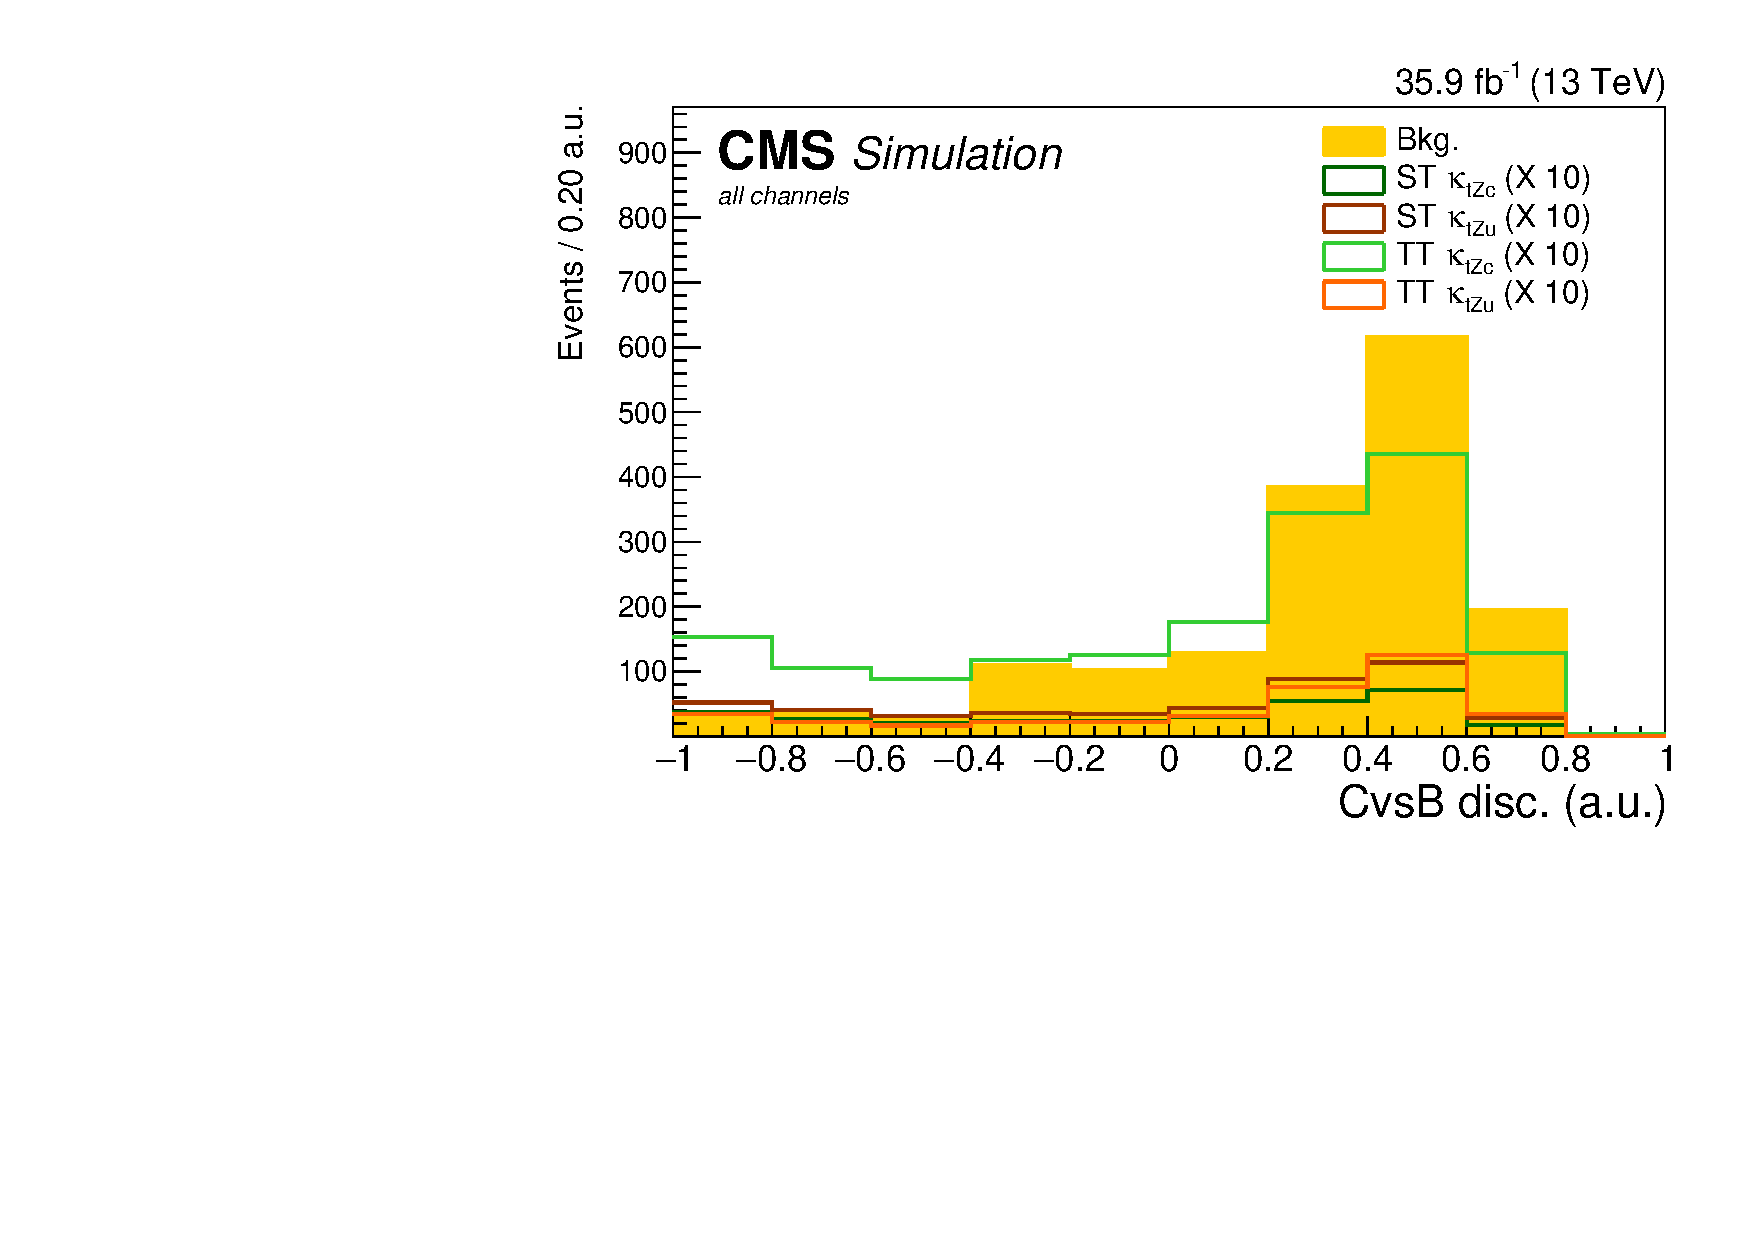
\includegraphics[width=0.49\linewidth]{7_Conclusion/Figures/charmtagging/3lepcontrol_dilep_CvsBdisc_all_Stack}
	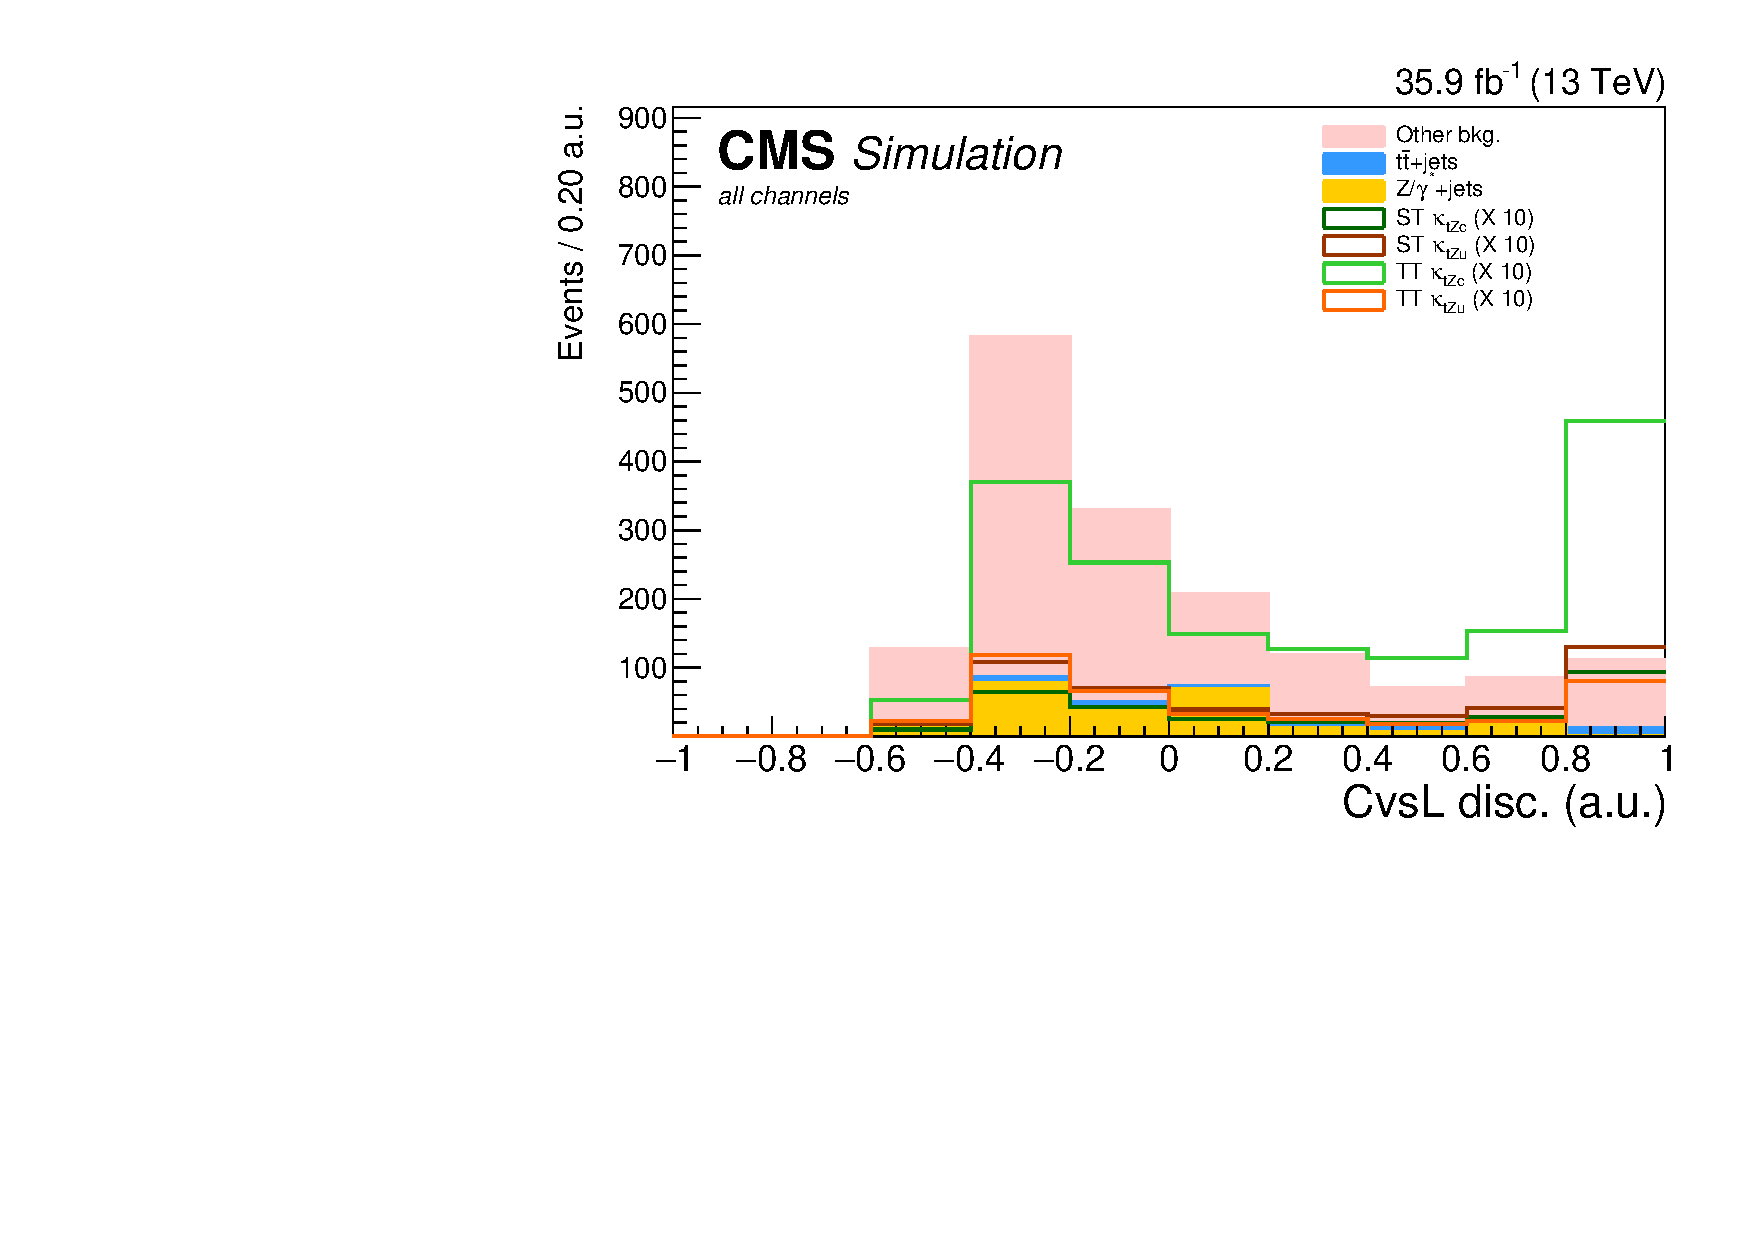
\includegraphics[width=0.49\linewidth]{7_Conclusion/Figures/charmtagging/3lepcontrol_dilep_CvsLdisc_all_Stack}
		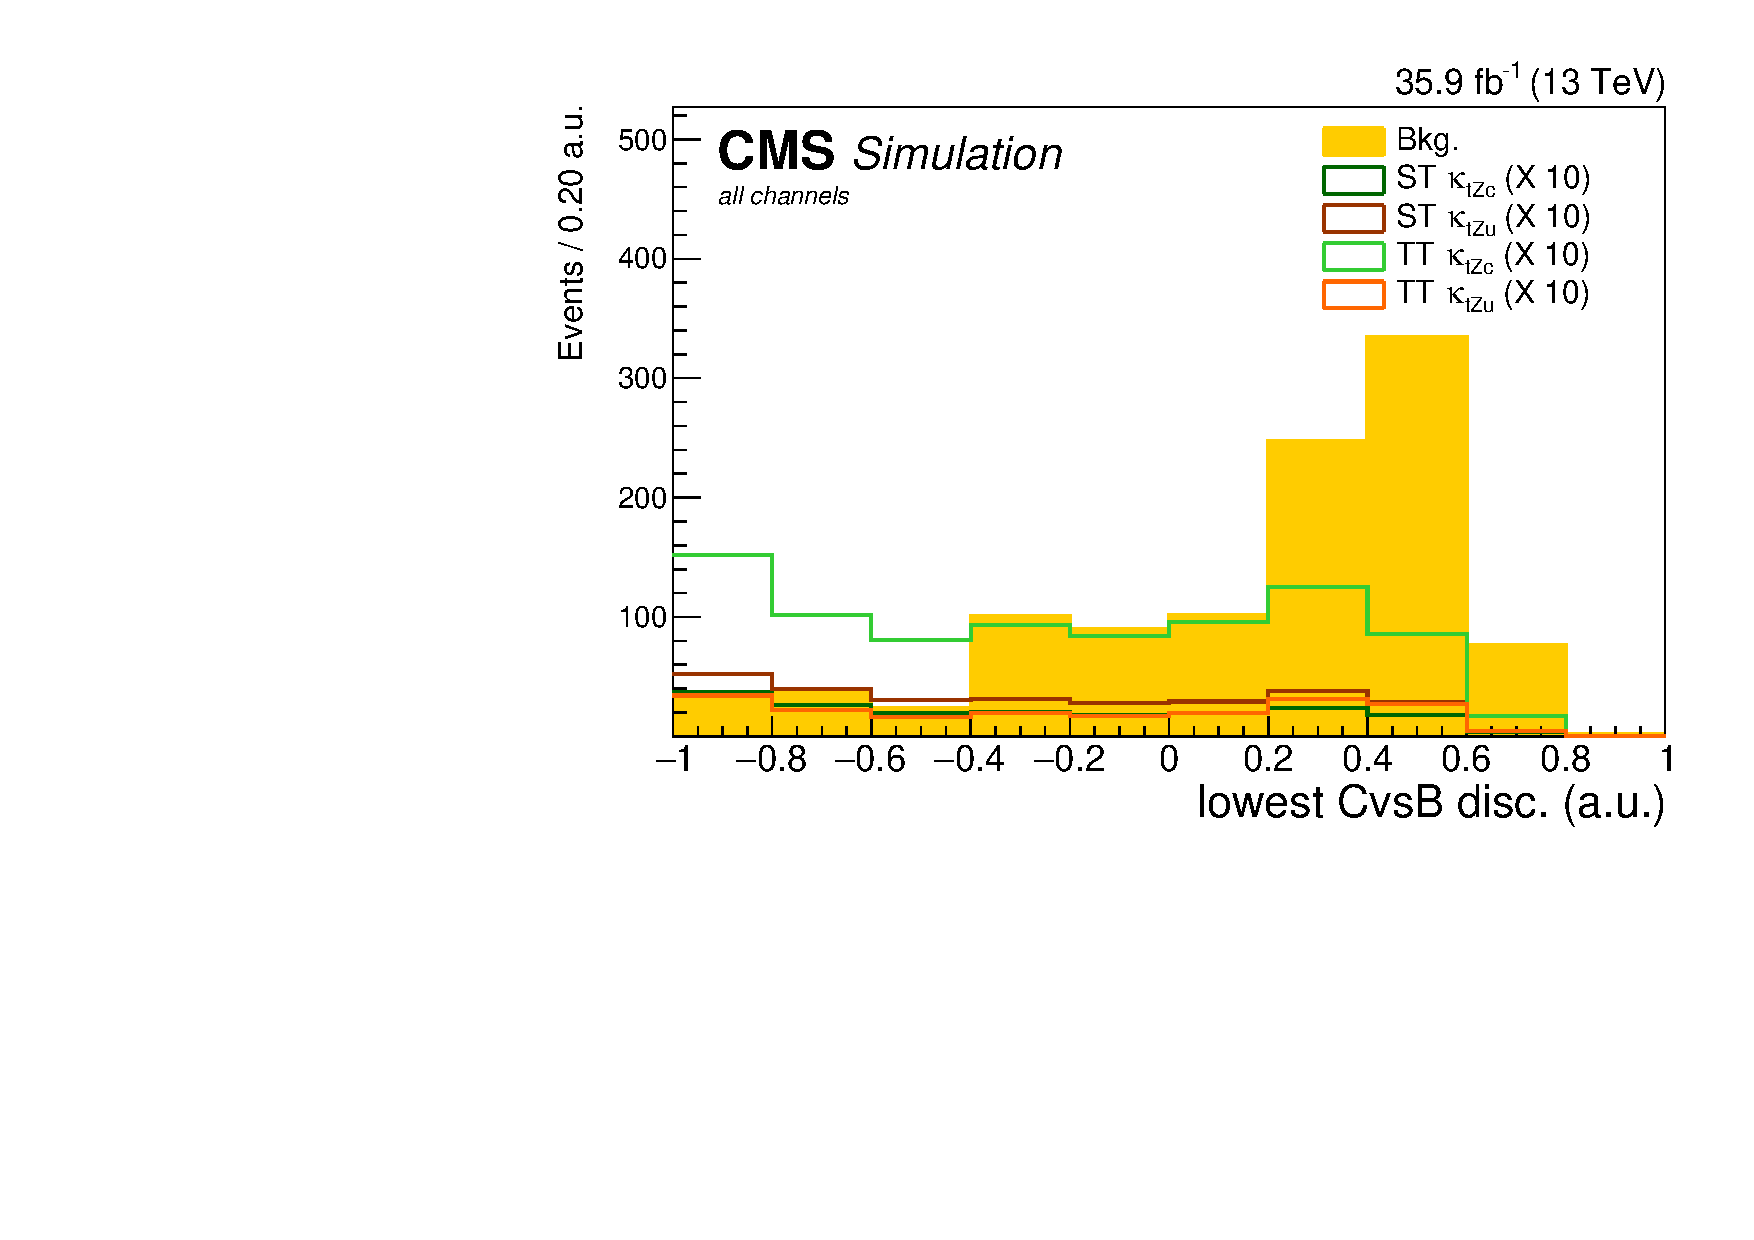
\includegraphics[width=0.49\linewidth]{7_Conclusion/Figures/charmtagging/3lepcontrol_dilep_CvsBdiscLow_all_Stack}
	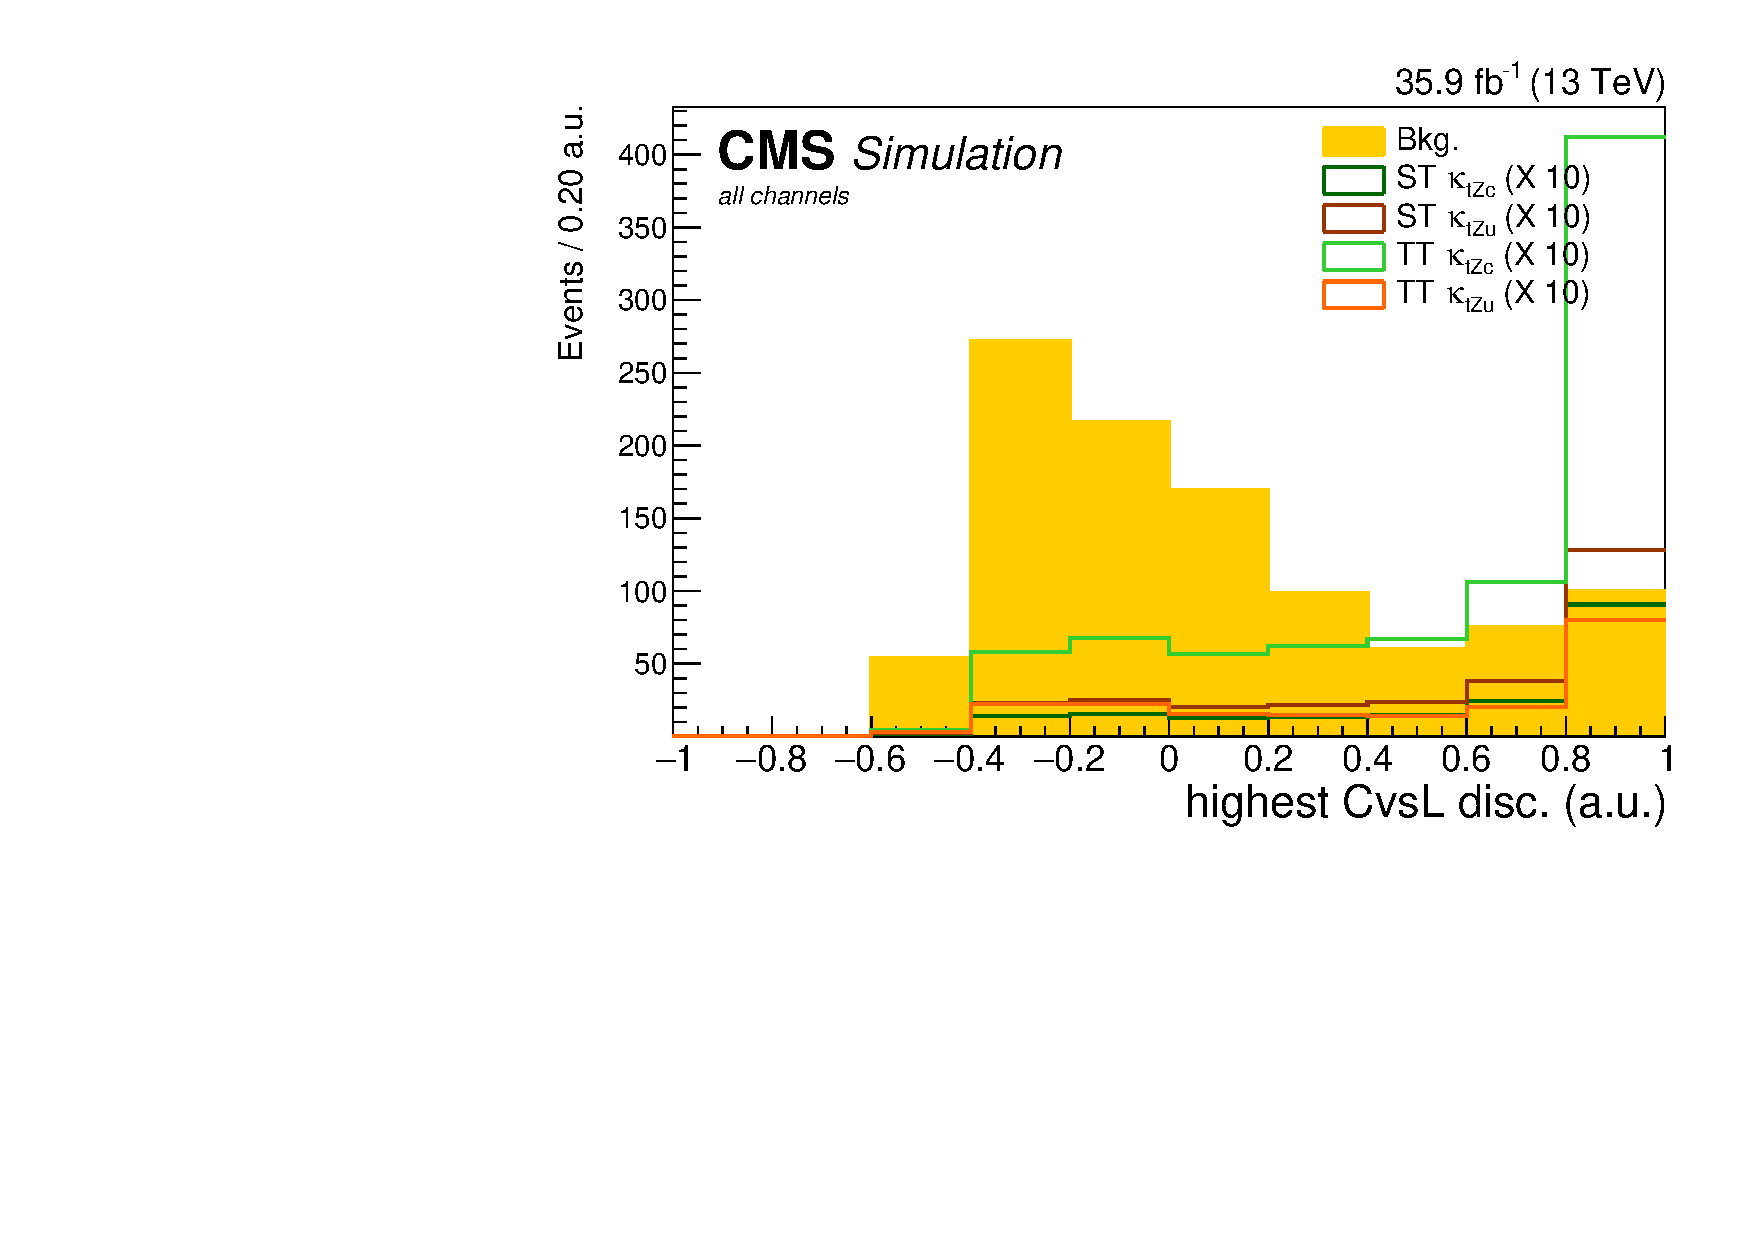
\includegraphics[width=0.49\linewidth]{7_Conclusion/Figures/charmtagging/3lepcontrol_dilep_CvsLdiscHigh_all_Stack}

	\caption{Distributions of the CvsB and CvsL discriminants after a three-lepton, for which a lepton pair is compatible with the Z boson, selection with jets.}
	\label{fig:ctagging}
\end{figure}

\begin{figure}[htbp]  % OutputPlots/171128_1746   of 1913
	\centering
	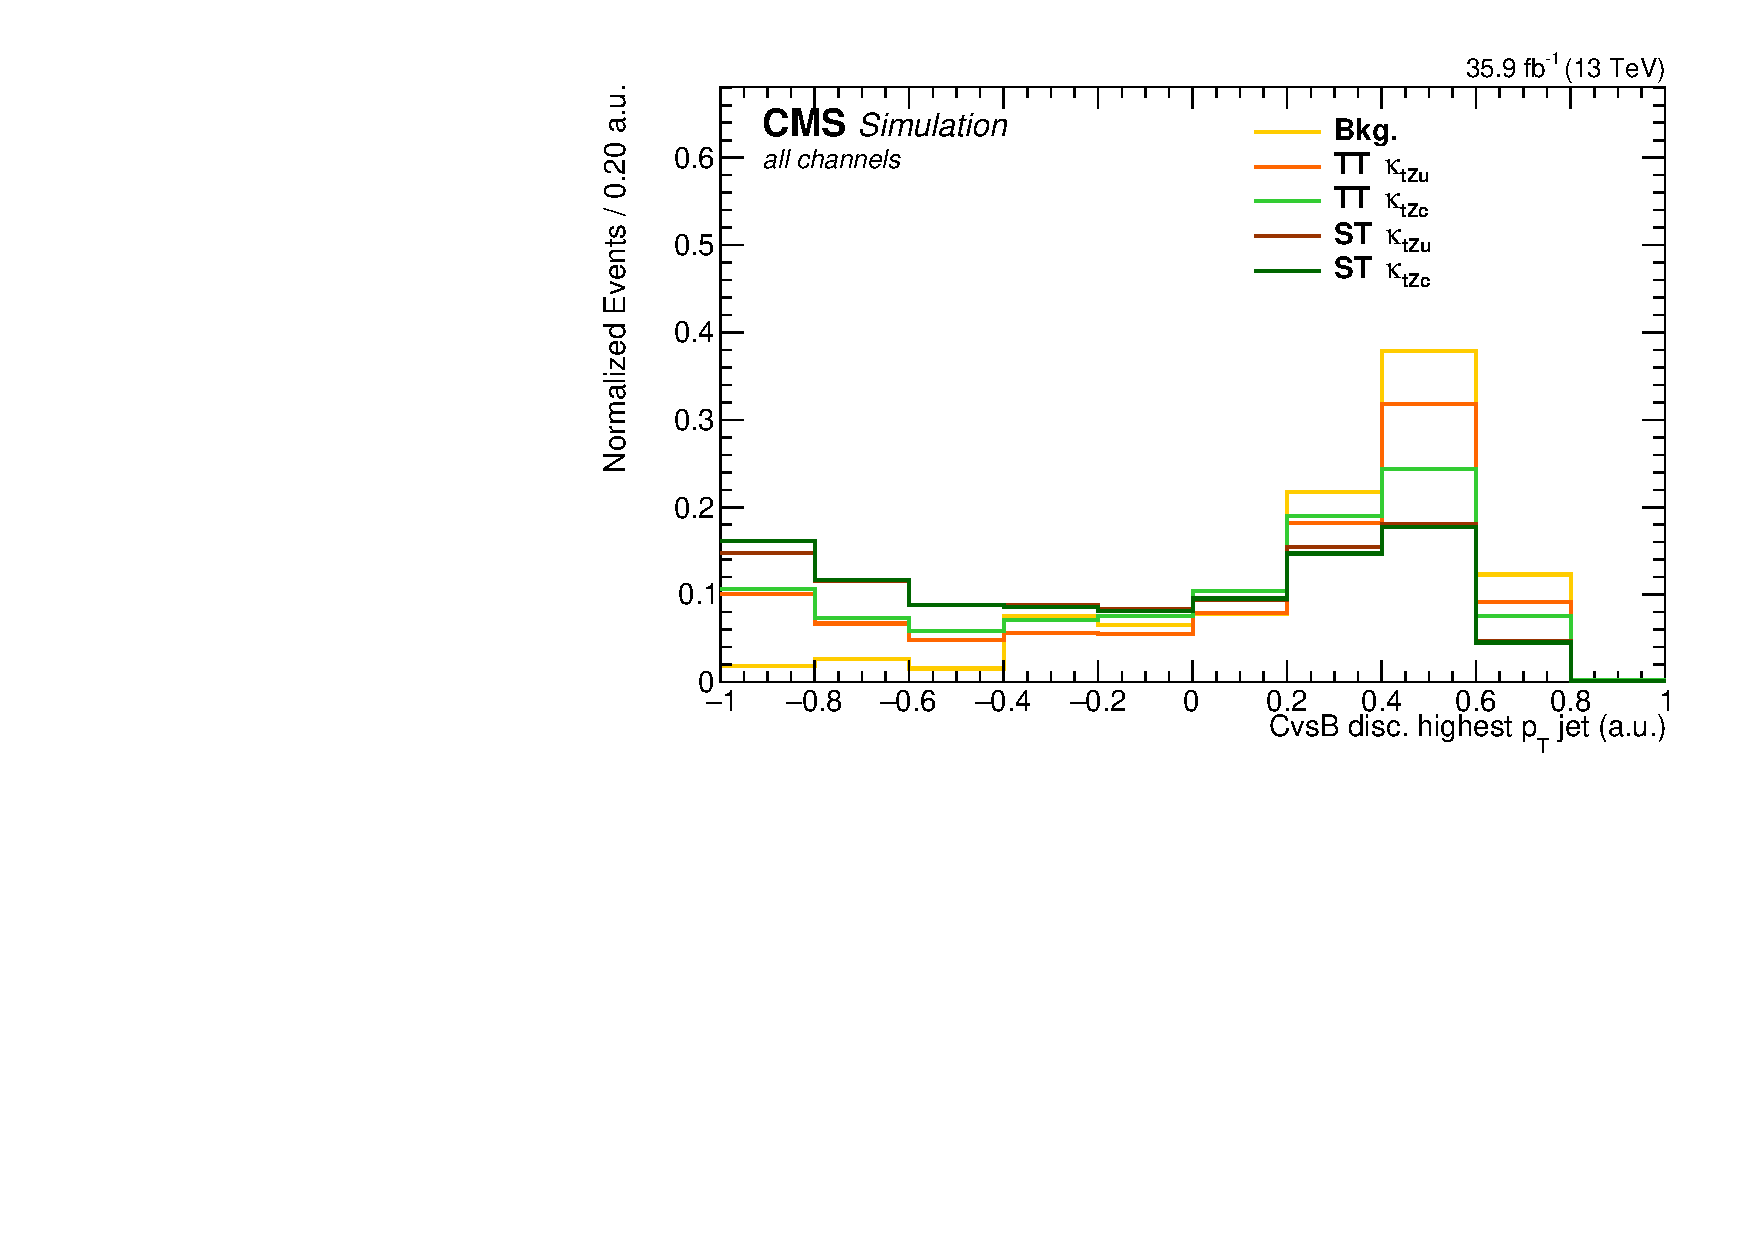
\includegraphics[width=0.49\linewidth]{7_Conclusion/Figures/charmtagging/3lepcontrol_dilep_CvsBdisc_0jet_all_Normalized}
	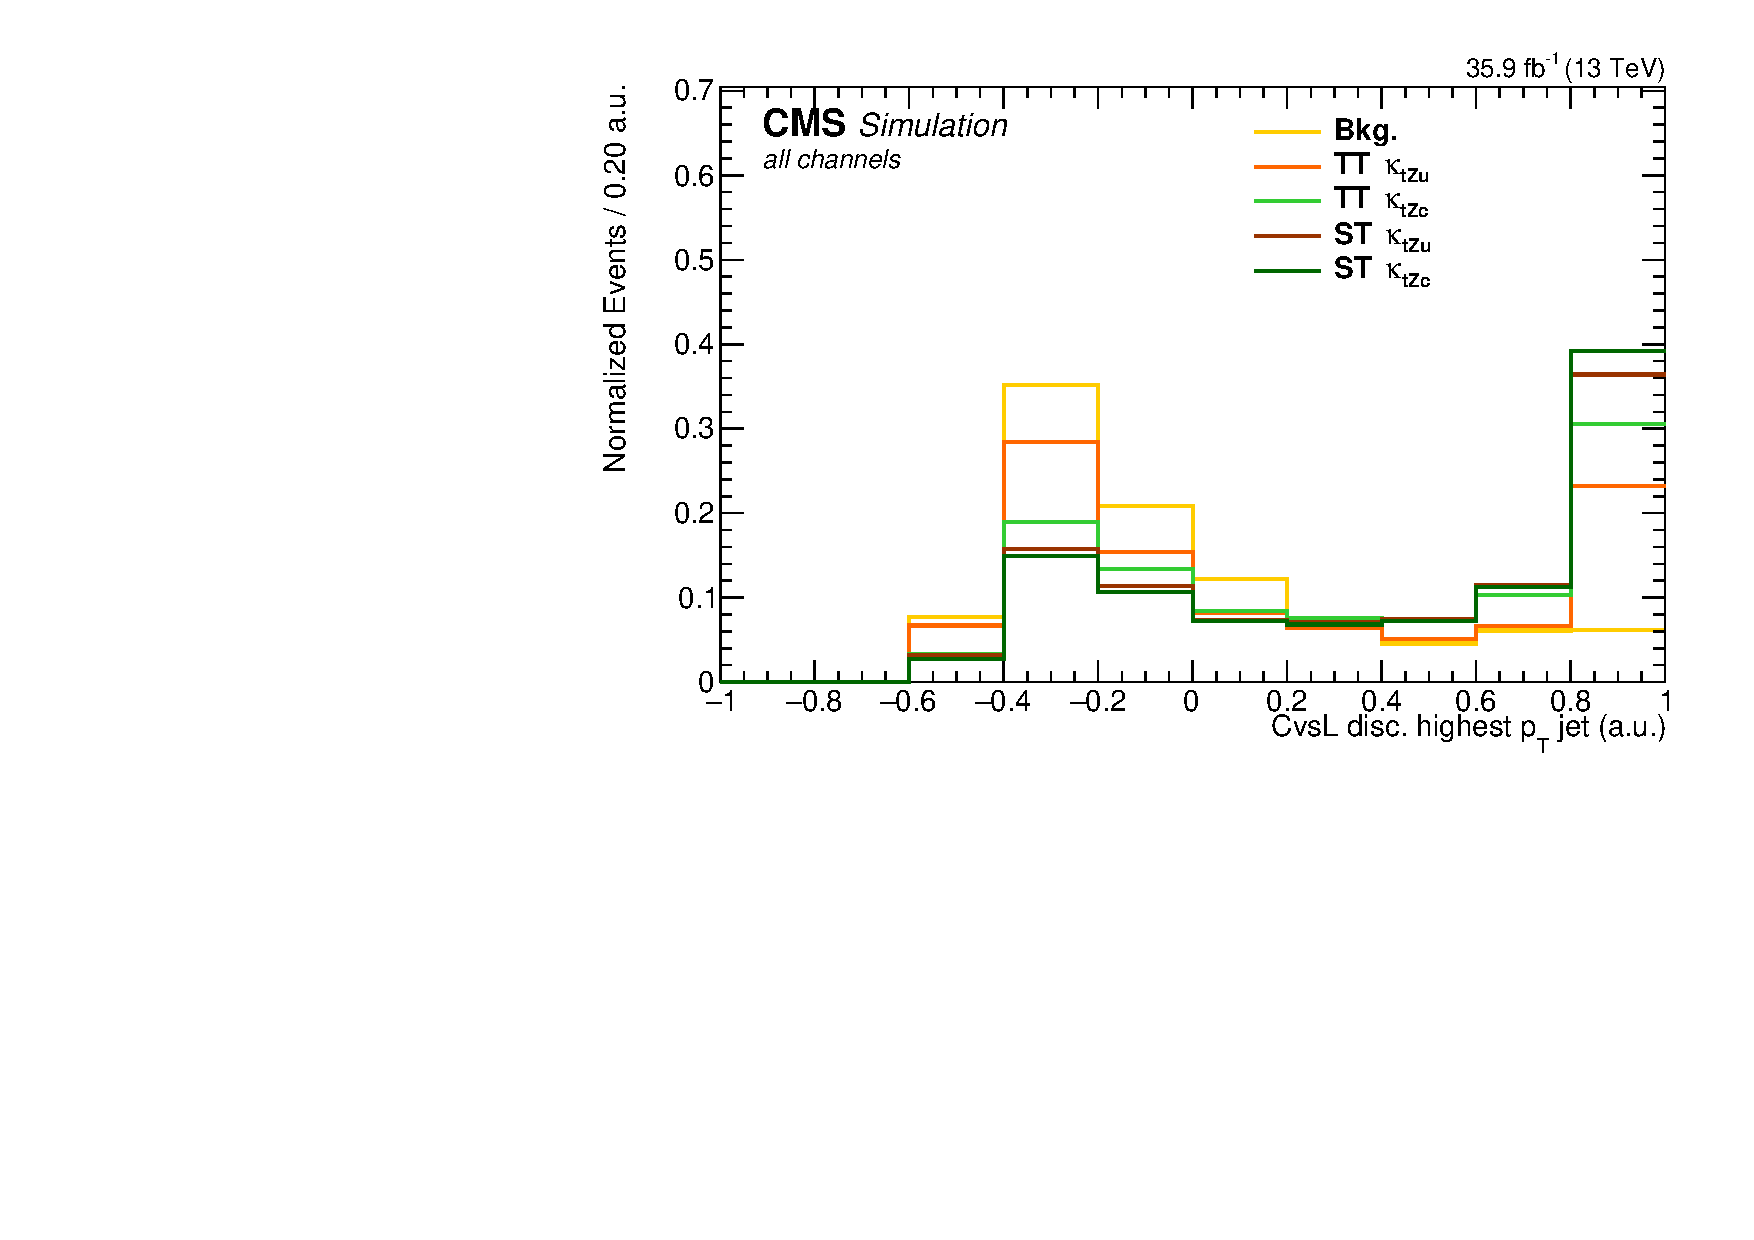
\includegraphics[width=0.49\linewidth]{7_Conclusion/Figures/charmtagging/3lepcontrol_dilep_CvsLdisc_0jet_all_Normalized}
	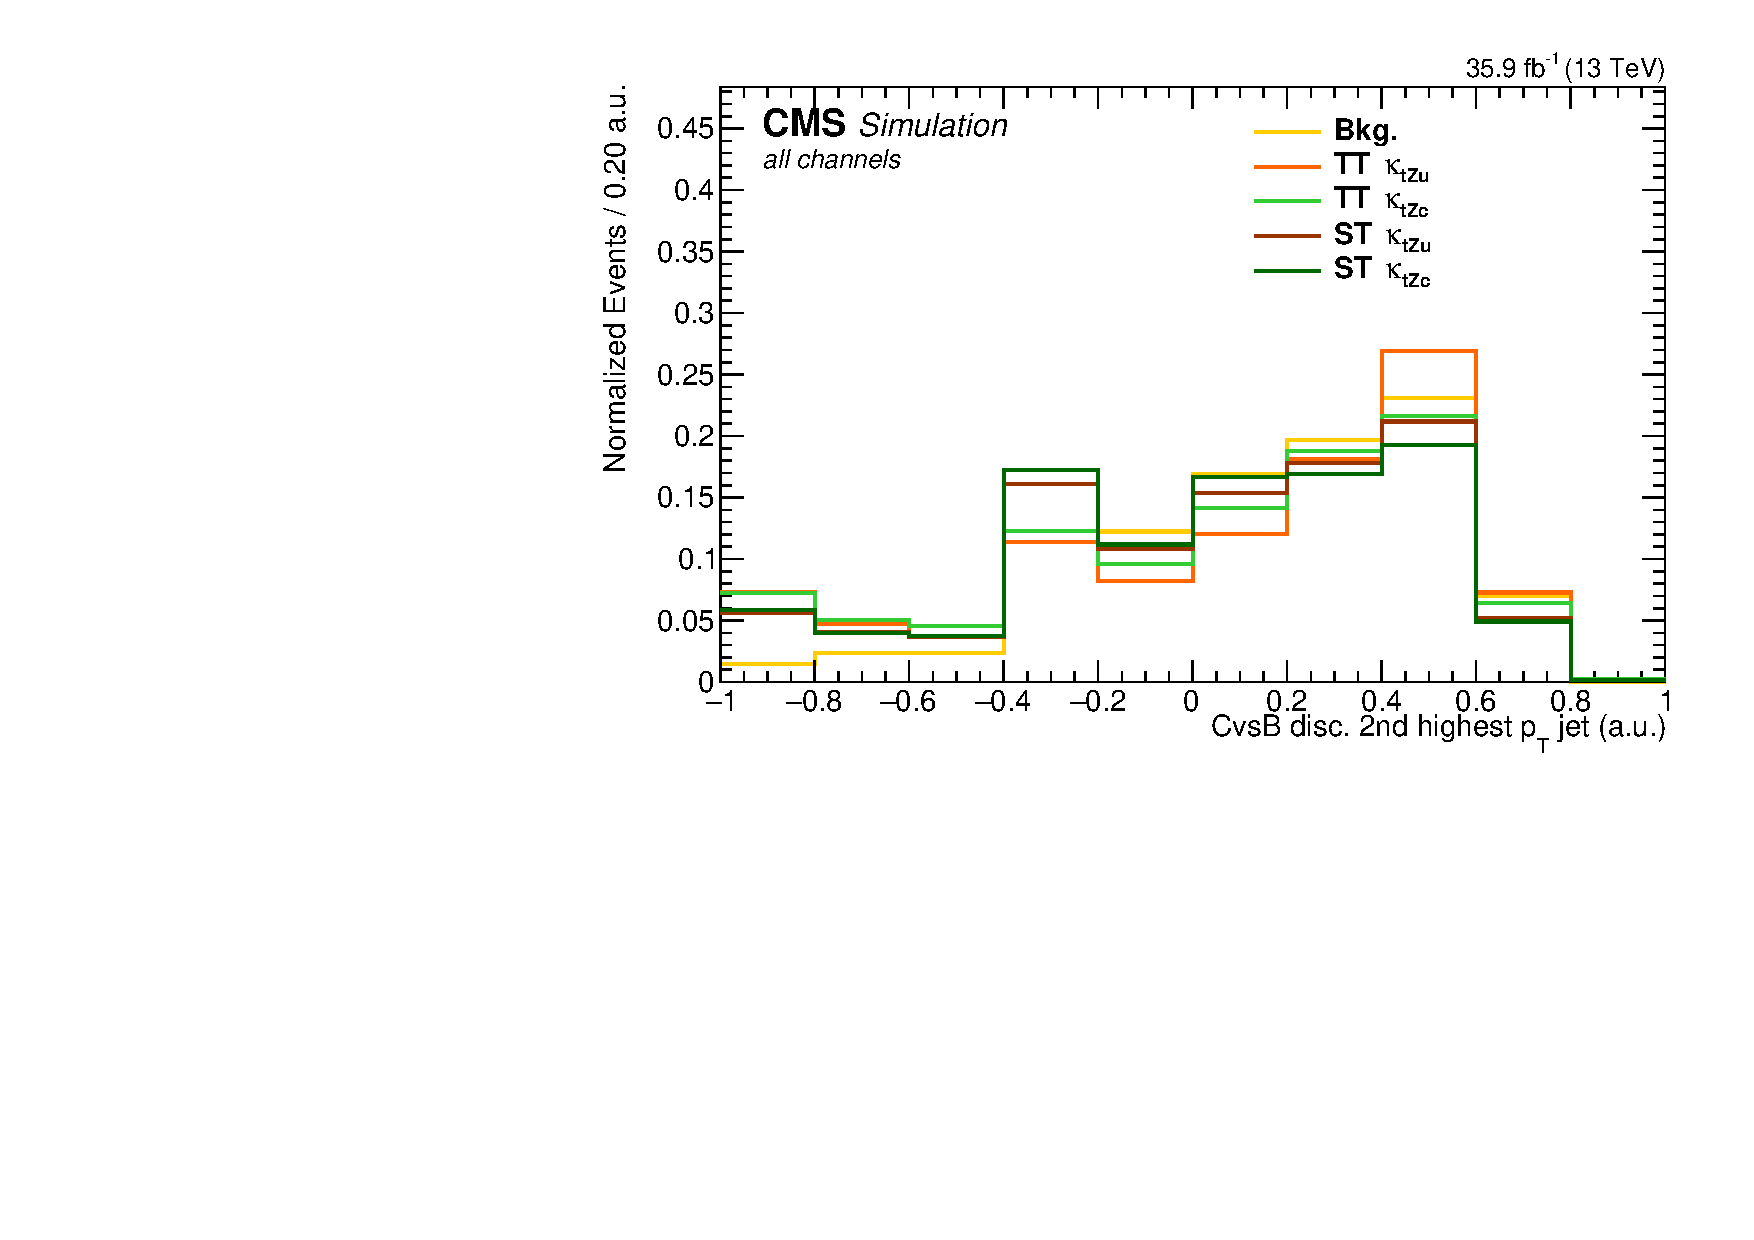
\includegraphics[width=0.49\linewidth]{7_Conclusion/Figures/charmtagging/3lepcontrol_dilep_CvsBdisc_1jet_all_Normalized}
	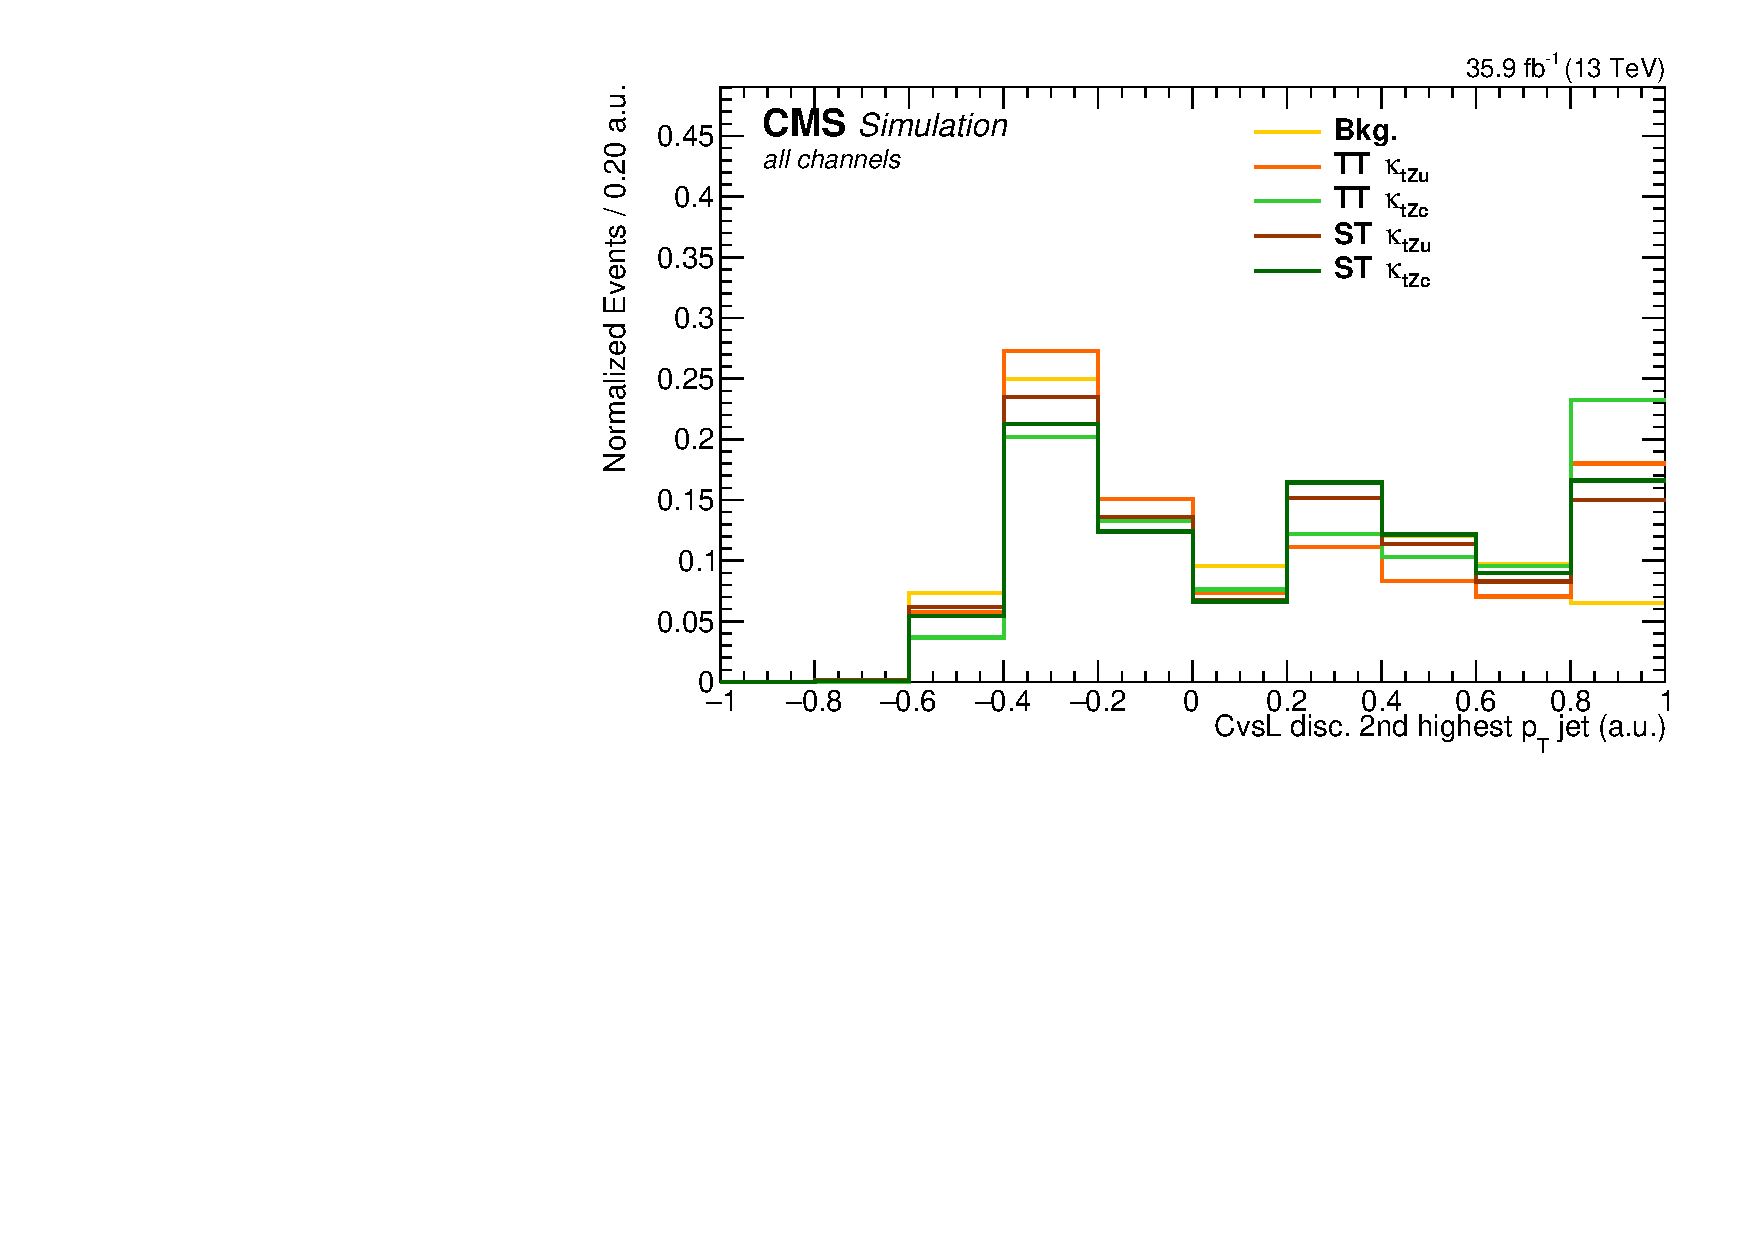
\includegraphics[width=0.49\linewidth]{7_Conclusion/Figures/charmtagging/3lepcontrol_dilep_CvsLdisc_1jet_all_Normalized}
	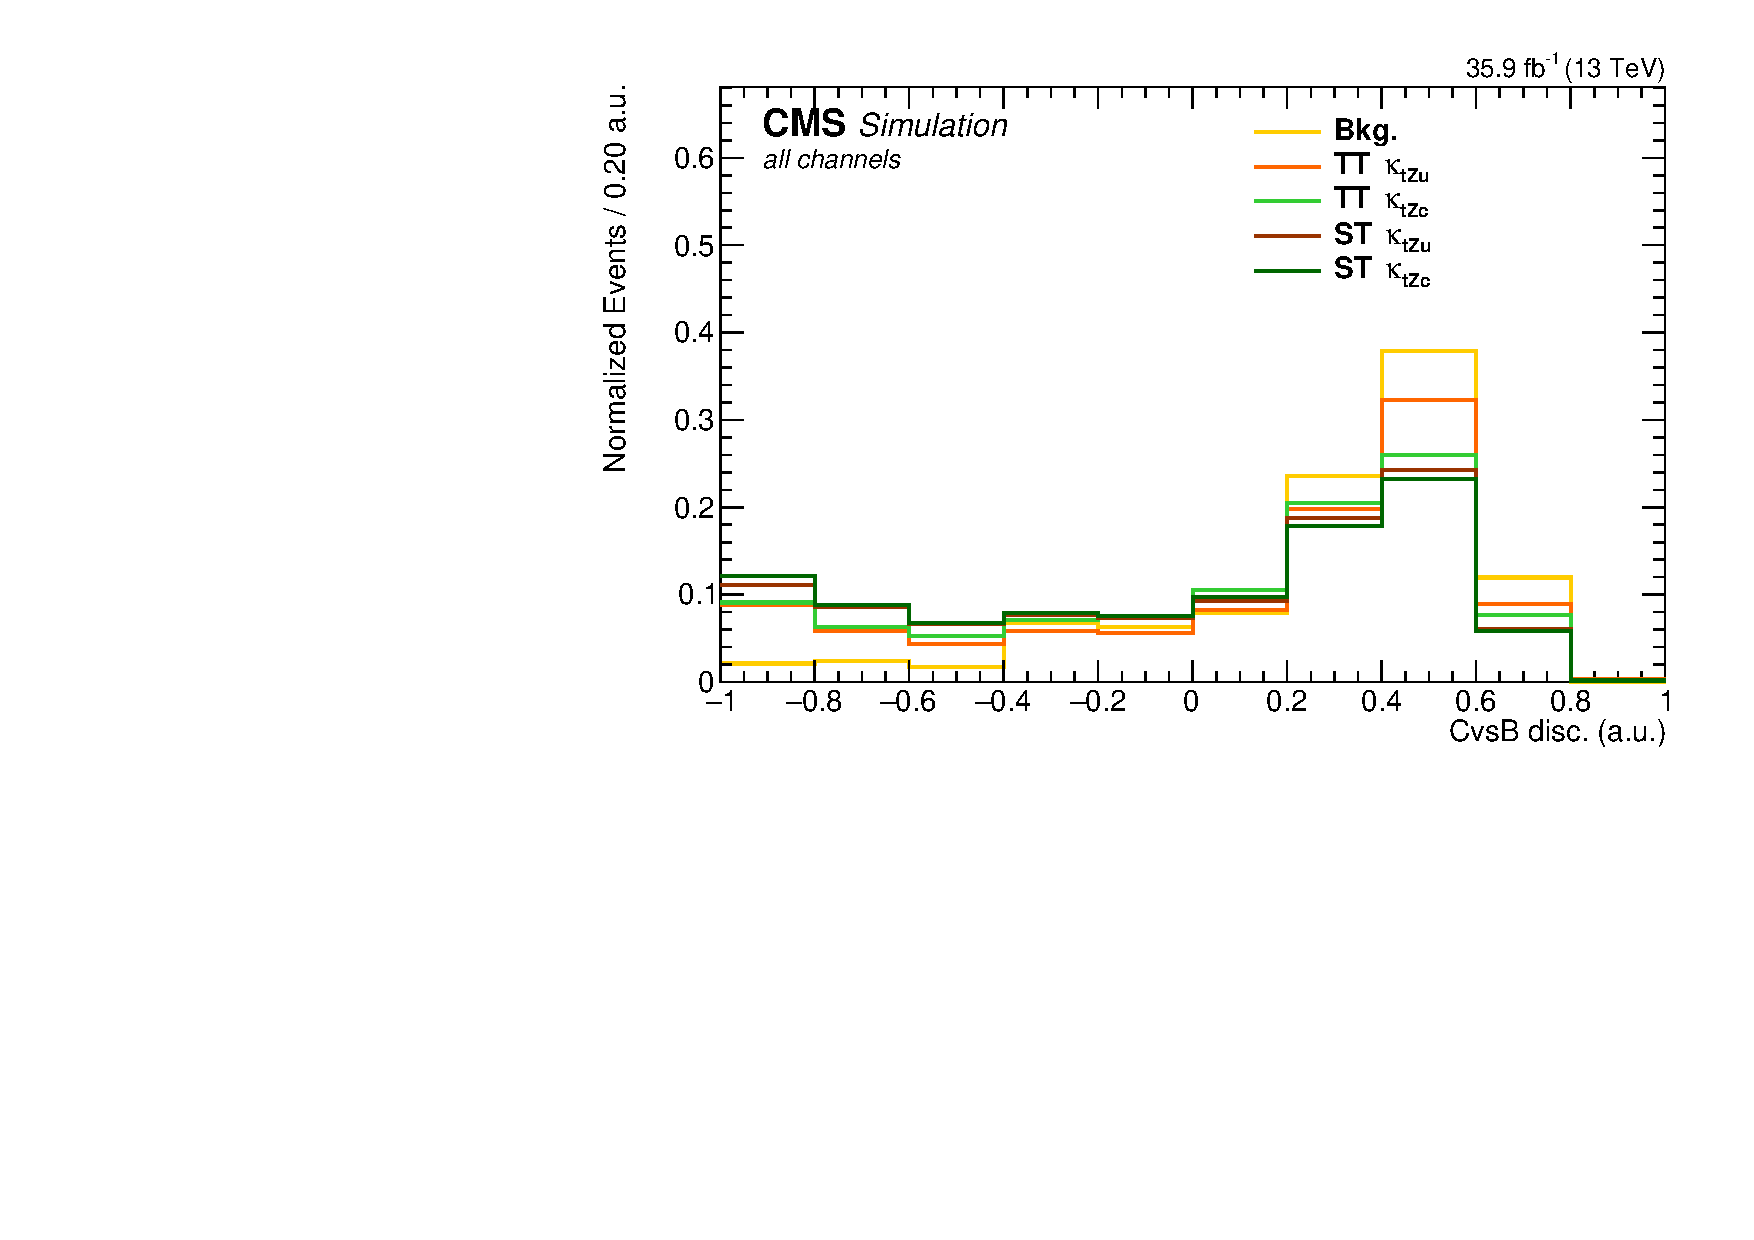
\includegraphics[width=0.49\linewidth]{7_Conclusion/Figures/charmtagging/3lepcontrol_dilep_CvsBdisc_all_Normalized}
	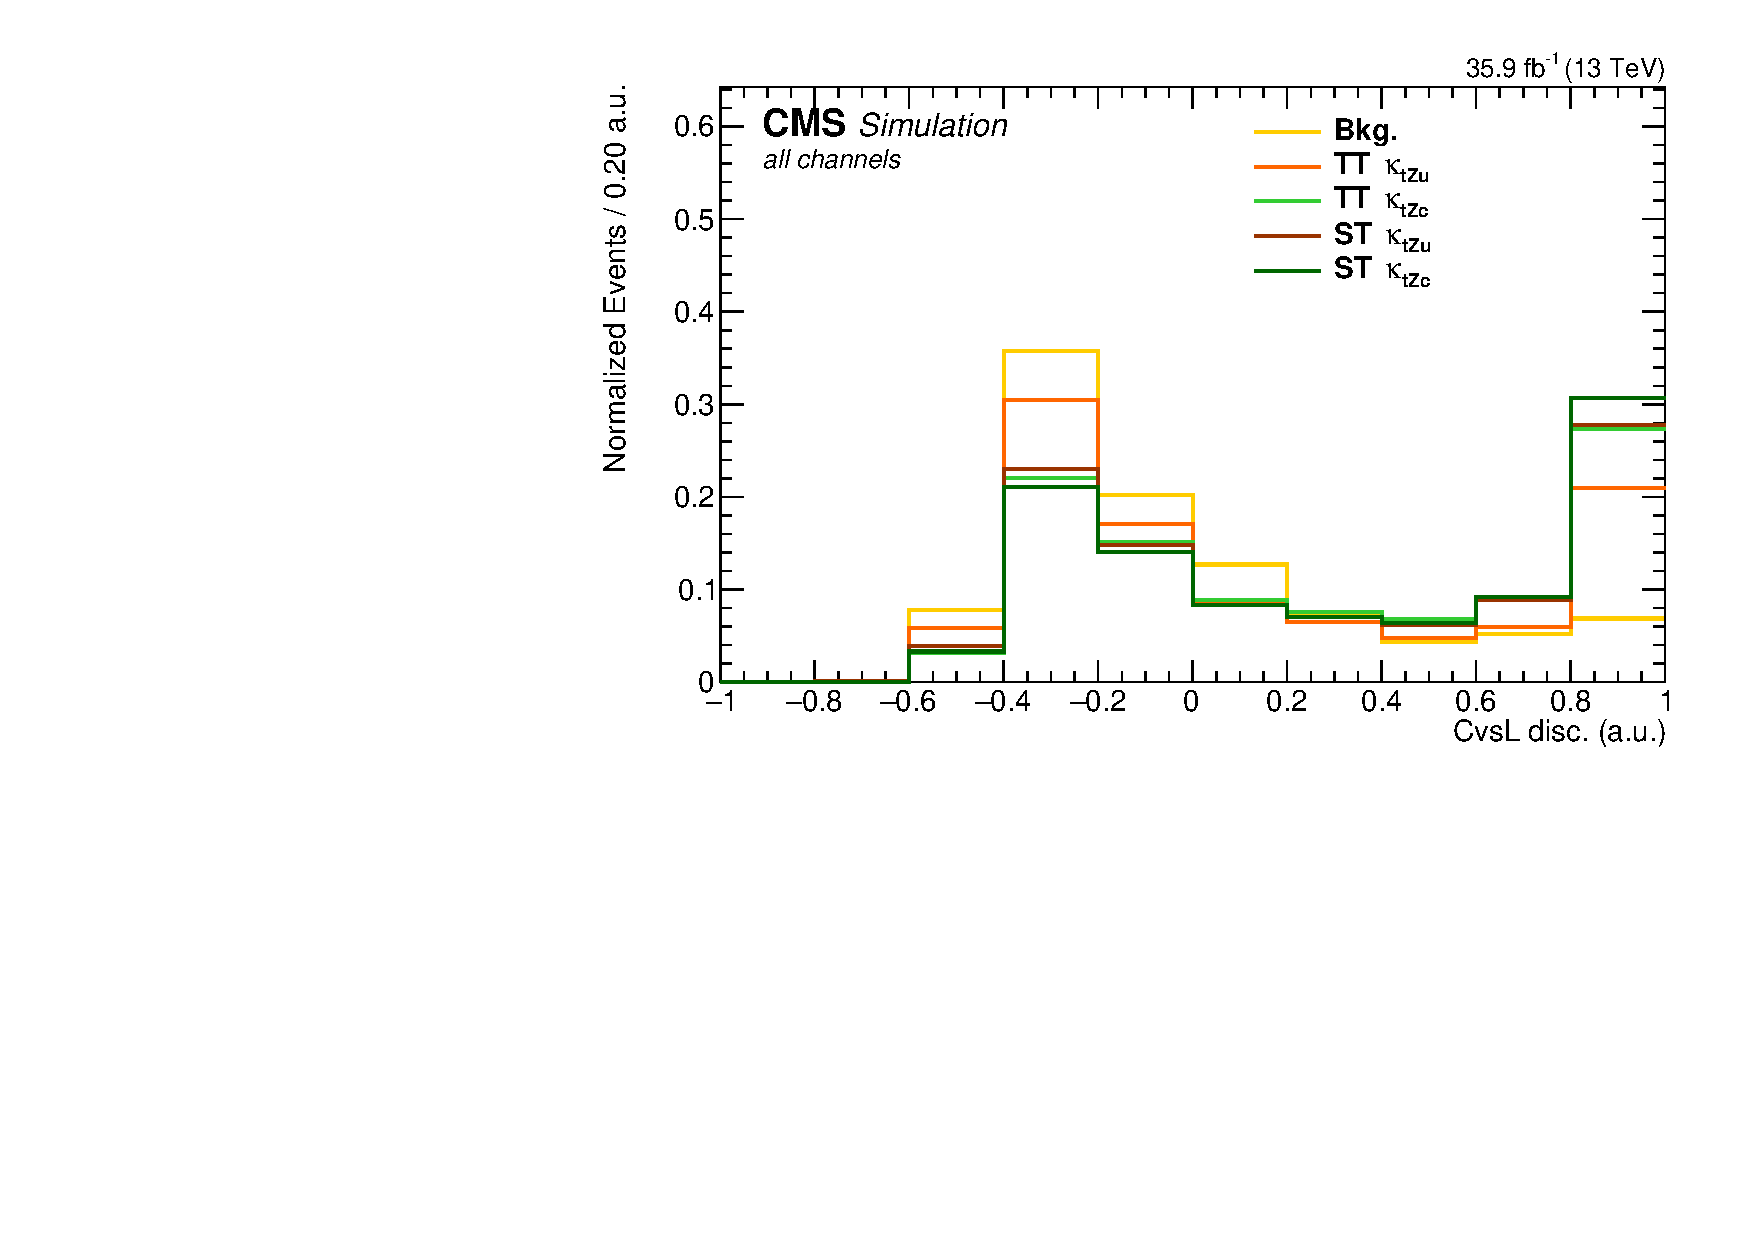
\includegraphics[width=0.49\linewidth]{7_Conclusion/Figures/charmtagging/3lepcontrol_dilep_CvsLdisc_all_Normalized}
	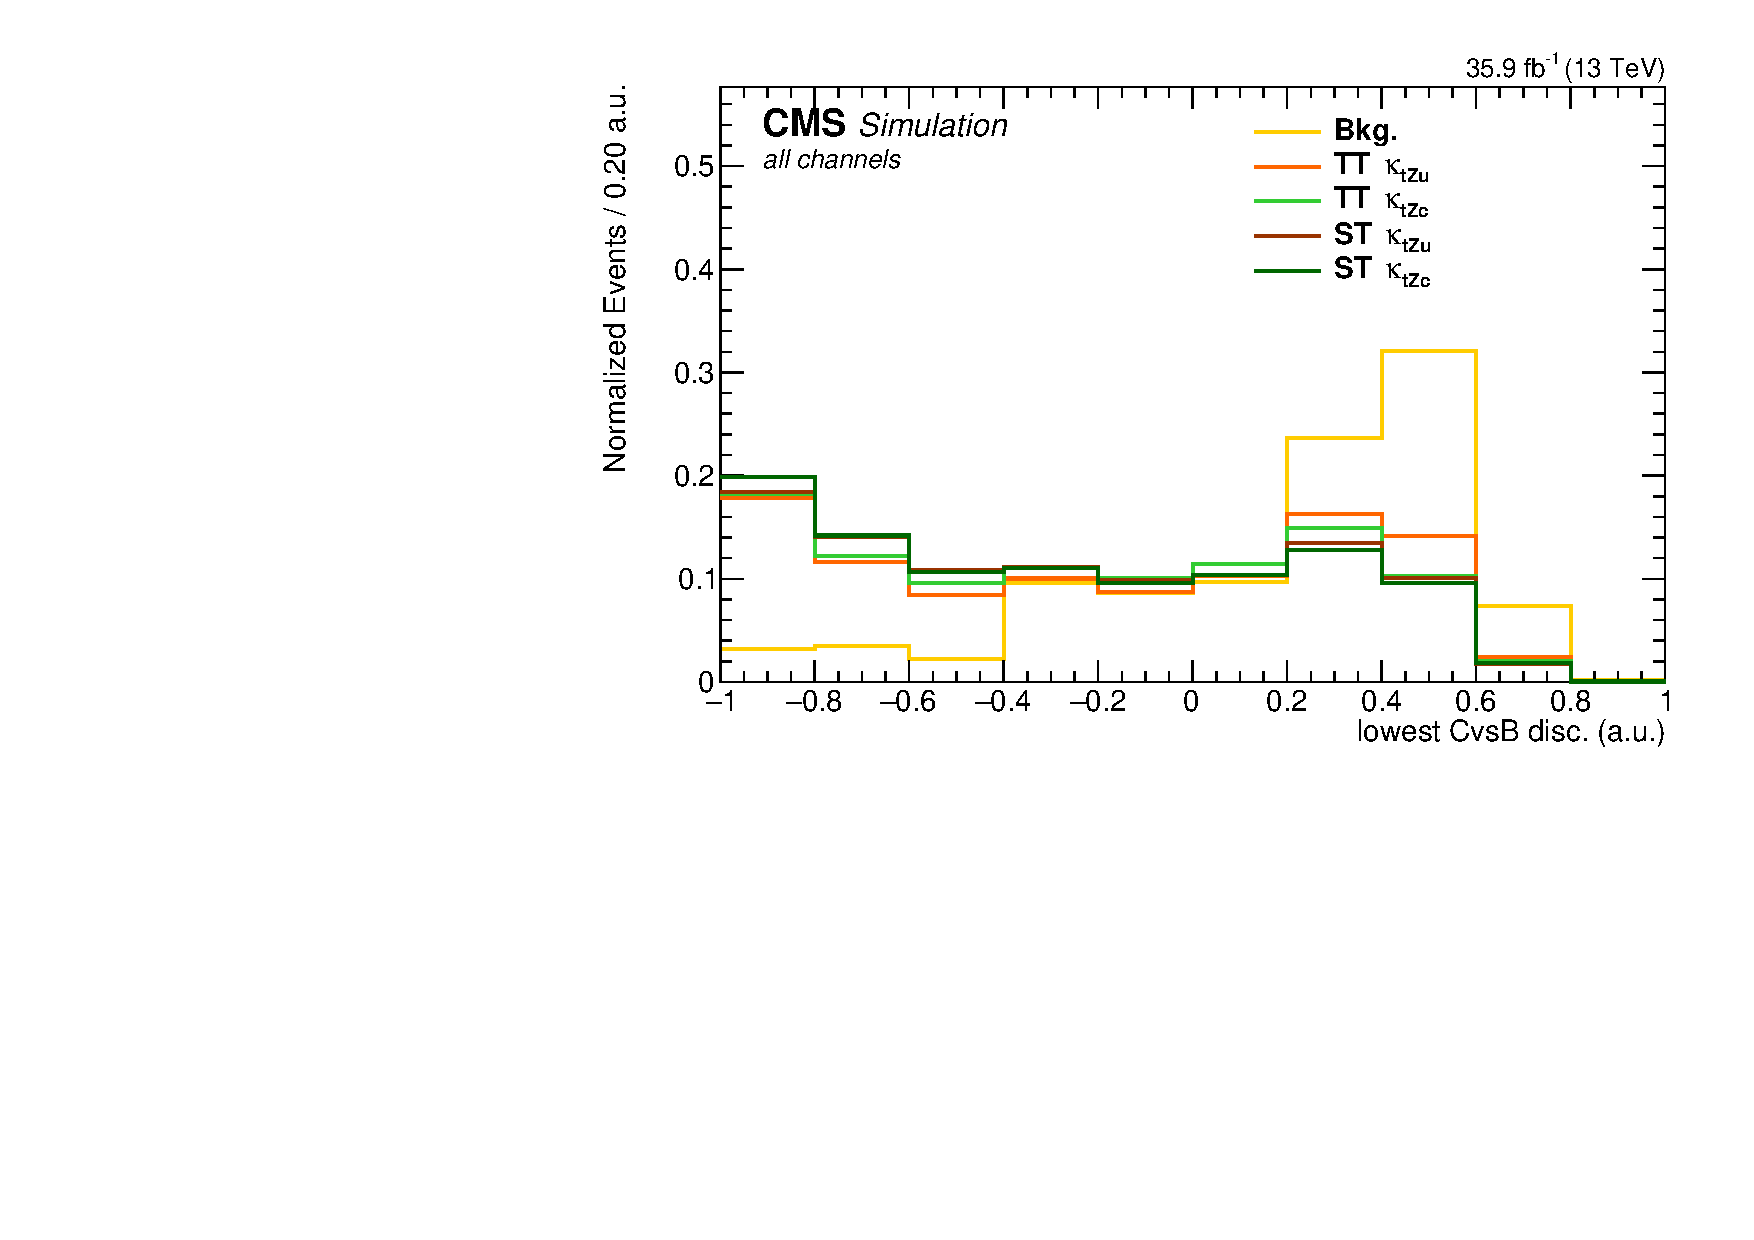
\includegraphics[width=0.49\linewidth]{7_Conclusion/Figures/charmtagging/3lepcontrol_dilep_CvsBdiscLow_all_Normalized}
	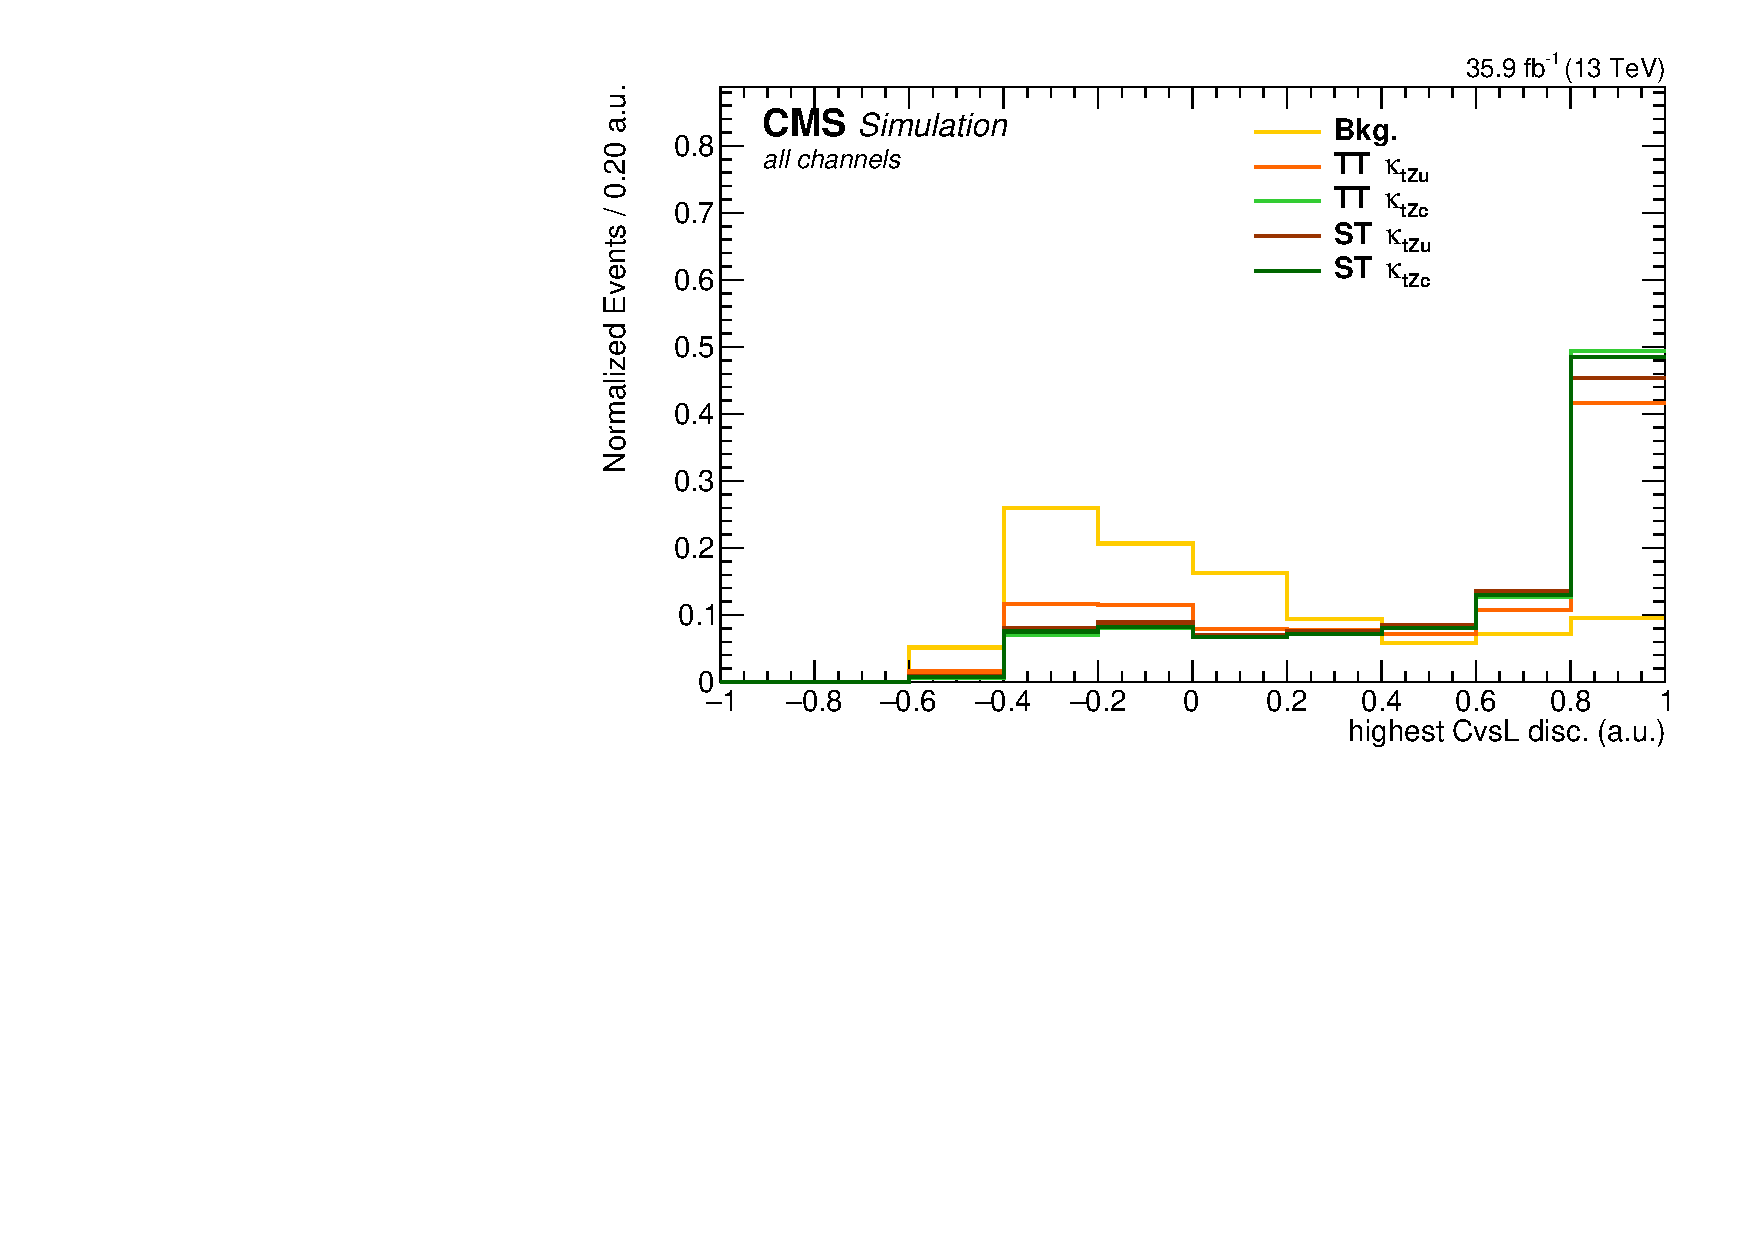
\includegraphics[width=0.49\linewidth]{7_Conclusion/Figures/charmtagging/3lepcontrol_dilep_CvsLdiscHigh_all_Normalized}
	
	\caption{Distributions of the CvsB and CvsL discriminants after a three-lepton, for which a lepton pair is compatible with the Z boson, selection with jets.}
	\label{fig:ctaggieng}
\end{figure}



Future colliders should be able to reach meaningful sensitivity for top-FCNC couplings. In \fig{fig:fcncupperlimitproj}, the sensitivity of the LHC at a centre-of-mass energy of 14 \TeV\ and 3000 \fbinv\ integrated luminosity (HL-LHC)~\cite{Agashe:2013hma}, as well as ILC/CLIC at a centre-of-mass energy of 500~\GeV\ and 500~\fbinv\ of integrated luminosity~\cite{Mangano:2016jyj}, the  Future Circular hadron Colliders at a centre-of-mass of 100 \TeV\ with an integrated luminosity of 10 ab$^{-1}$ (FCC-hh)~\cite{Agashe:2013hma}, the Future Circular electron positron Colliders at a centre-of-mass of 500~\GeV\ with an integrated luminosity of 10~ab$^{-1}$ (FCC-ee)~\cite{Khanpour:2014xla}, and the future Large Hadron electron Collider (LHeC) with a centre-of-mass of 14~\TeV\ and an integrated luminosity of 200 \fbinv~\cite{Liu:2015kkp} are shown. The sensitivities are originating from projections as well as sensitivity studies based on the changes in luminosity, energy, and trigger thresholds. 
\begin{comment}
The future large scale circular electron-positron collider (FCC-ee) would be one of the high- precision and high-luminosity machines which will be able to perform precise measurements on the Higgs boson, top-quark, Z and W bosons [43, 55]. Due to the expected large amount of data and large production rates, FCC-ee can provide an excellent opportunity for precise studies, in particular in the top quark sector. FCC-ee is designed to be working at the center-of-mass energy up to the tt ̄ threshold mass, i.e. √s = 350 GeV which is upgradeable to 500 GeV. The goal is to reach to a luminosity of L = 1.3 × 1034 cm−2s−1 [43, 55].
https://arxiv.org/pdf/1408.2090.pdf met feynman diagram

LHeC met feynman diagram https://arxiv.org/pdf/1507.03264.pdf

CLIC arXiv:1604.08122 en https://arxiv.org/pdf/1611.04492.pdf https://arxiv.org/pdf/1604.08122.pdf

HL LHC http://iopscience.iop.org/article/10.1088/1742-6596/706/2/022002/pdf

uitleg BSM model https://arxiv.org/pdf/1311.2028.pdf  (snowmass)

Kirill https://indico.cern.ch/event/659310/contributions/2690162/attachments/1527542/2389404/kskovpenTOP2017.pdf

atlas thesis https://cds.cern.ch/record/2272850/files/CERN-THESIS-2016-313.pdf
\end{comment}
\begin{figure}[htbp]
	\centering
	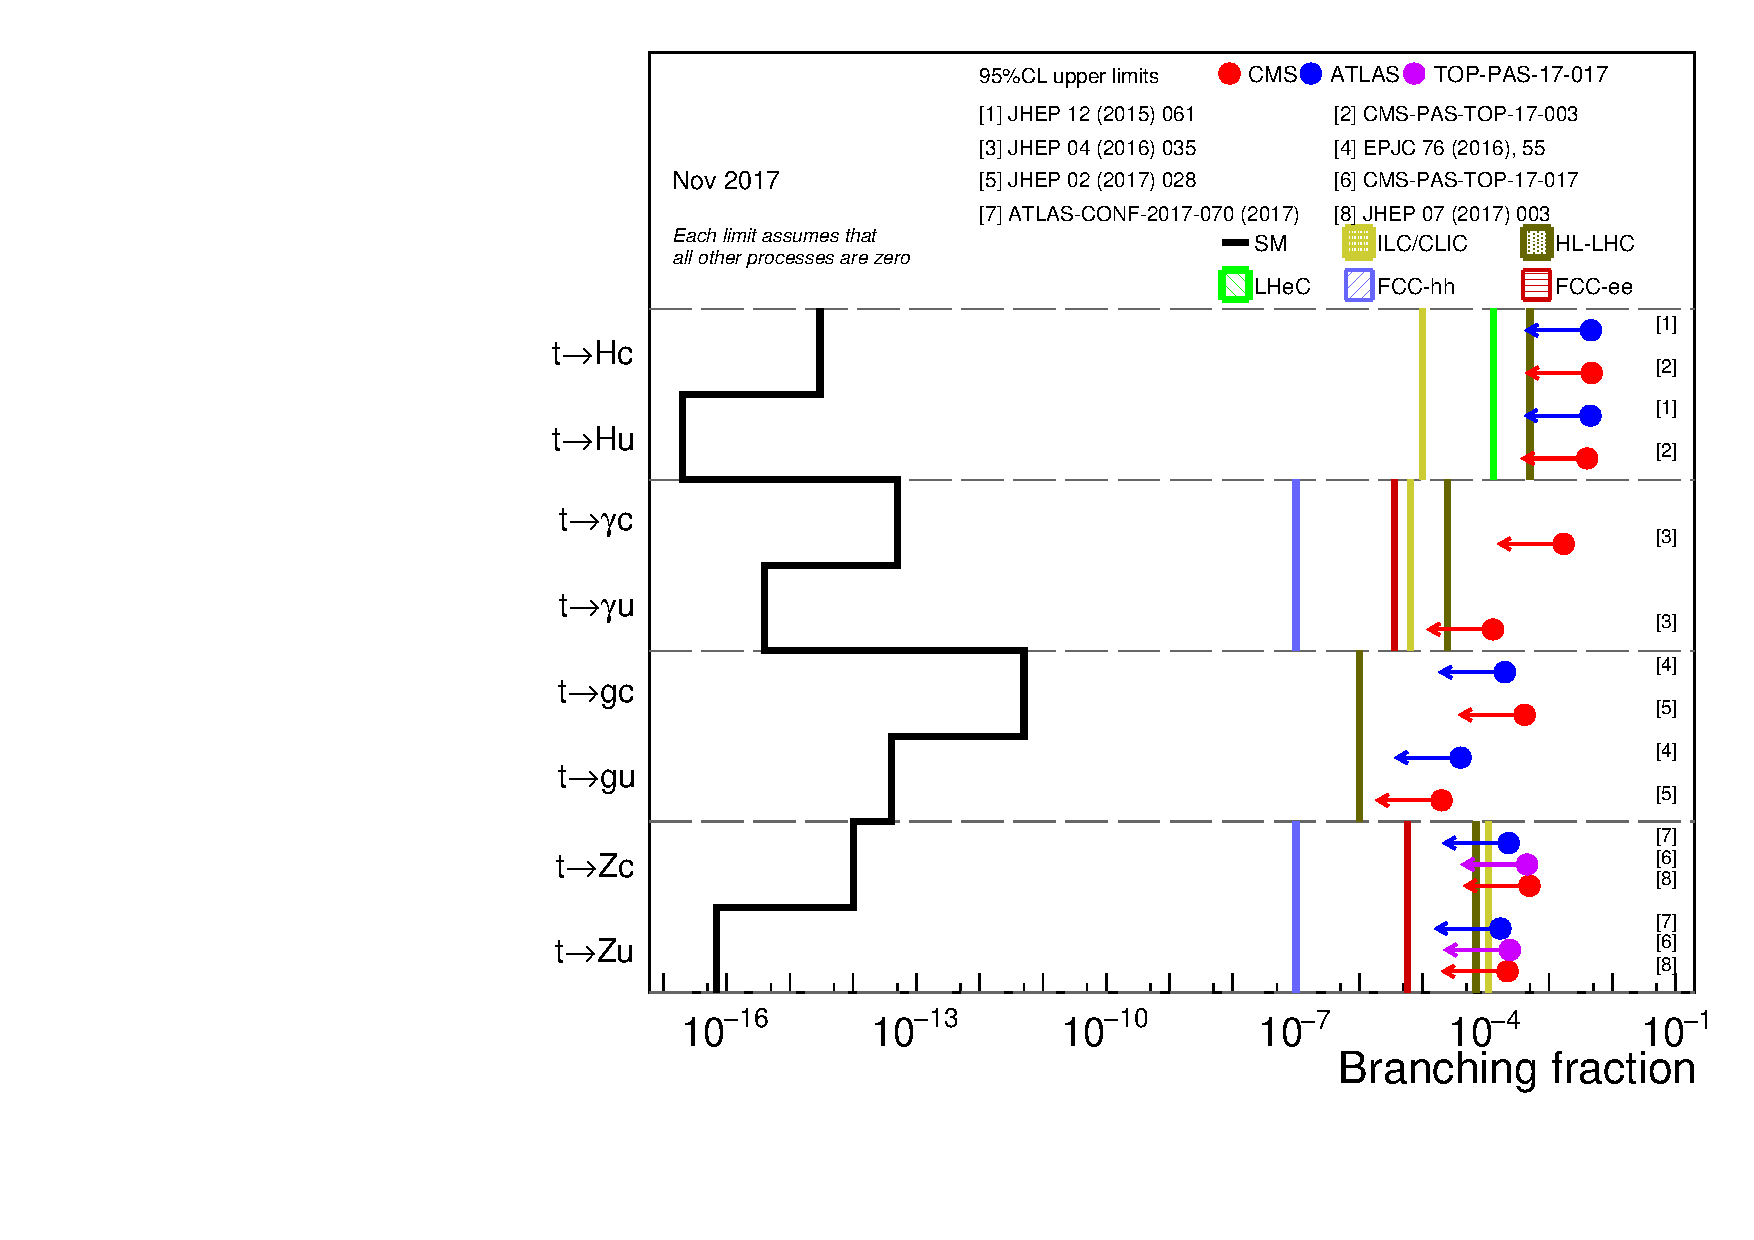
\includegraphics[width=.8\linewidth]{7_Conclusion/Figures/fcnc_upperlimits_proj.pdf}
	\caption{Summary of the most stringent upper limits on top-FCNC interactions at 95\% CL upper limits from CMS (red) and ATLAS (blue) at a centre-of-mass of 8 and 13 \TeV. The results from this thesis are shown in purple. A comparison between the projections for future colliders and the current experimental limits is shown. Figure adapted from \cite{summarywiki}. The projections are taken from \cite{Liu:2015kkp,Agashe:2013hma,Khanpour:2014xla,Mangano:2016jyj}.}
	\label{fig:fcncupperlimitproj}
\end{figure}


Instead of hadron colliders, one could also look at future lepton colliders such as the FCC-ee, where the signal $\Pep\Pem \rightarrow \PZ/\Pgamma \rightarrow \Ptop \APquark \: (\APtop\Pquark)$ can occur.  The FCC-ee would be one of the high luminosity and high precision machines and would be able to perform precise measurements of the top quark, Higgs, \PZ\, and \PW\  bosons. Its large production rates create an excellent environment for precise studies in the top quark section  of the Standard Model. In Ref.~\cite{Khanpour:2014xla}, a study of the FCNC \tZq\ single top quark production is done at different centre-of-mass energies and for different integrated luminosities. In \fig{fig:fcncupperlimitproj}, their most stringent results are shown. 

%\begin{figure}
%	\centering
%	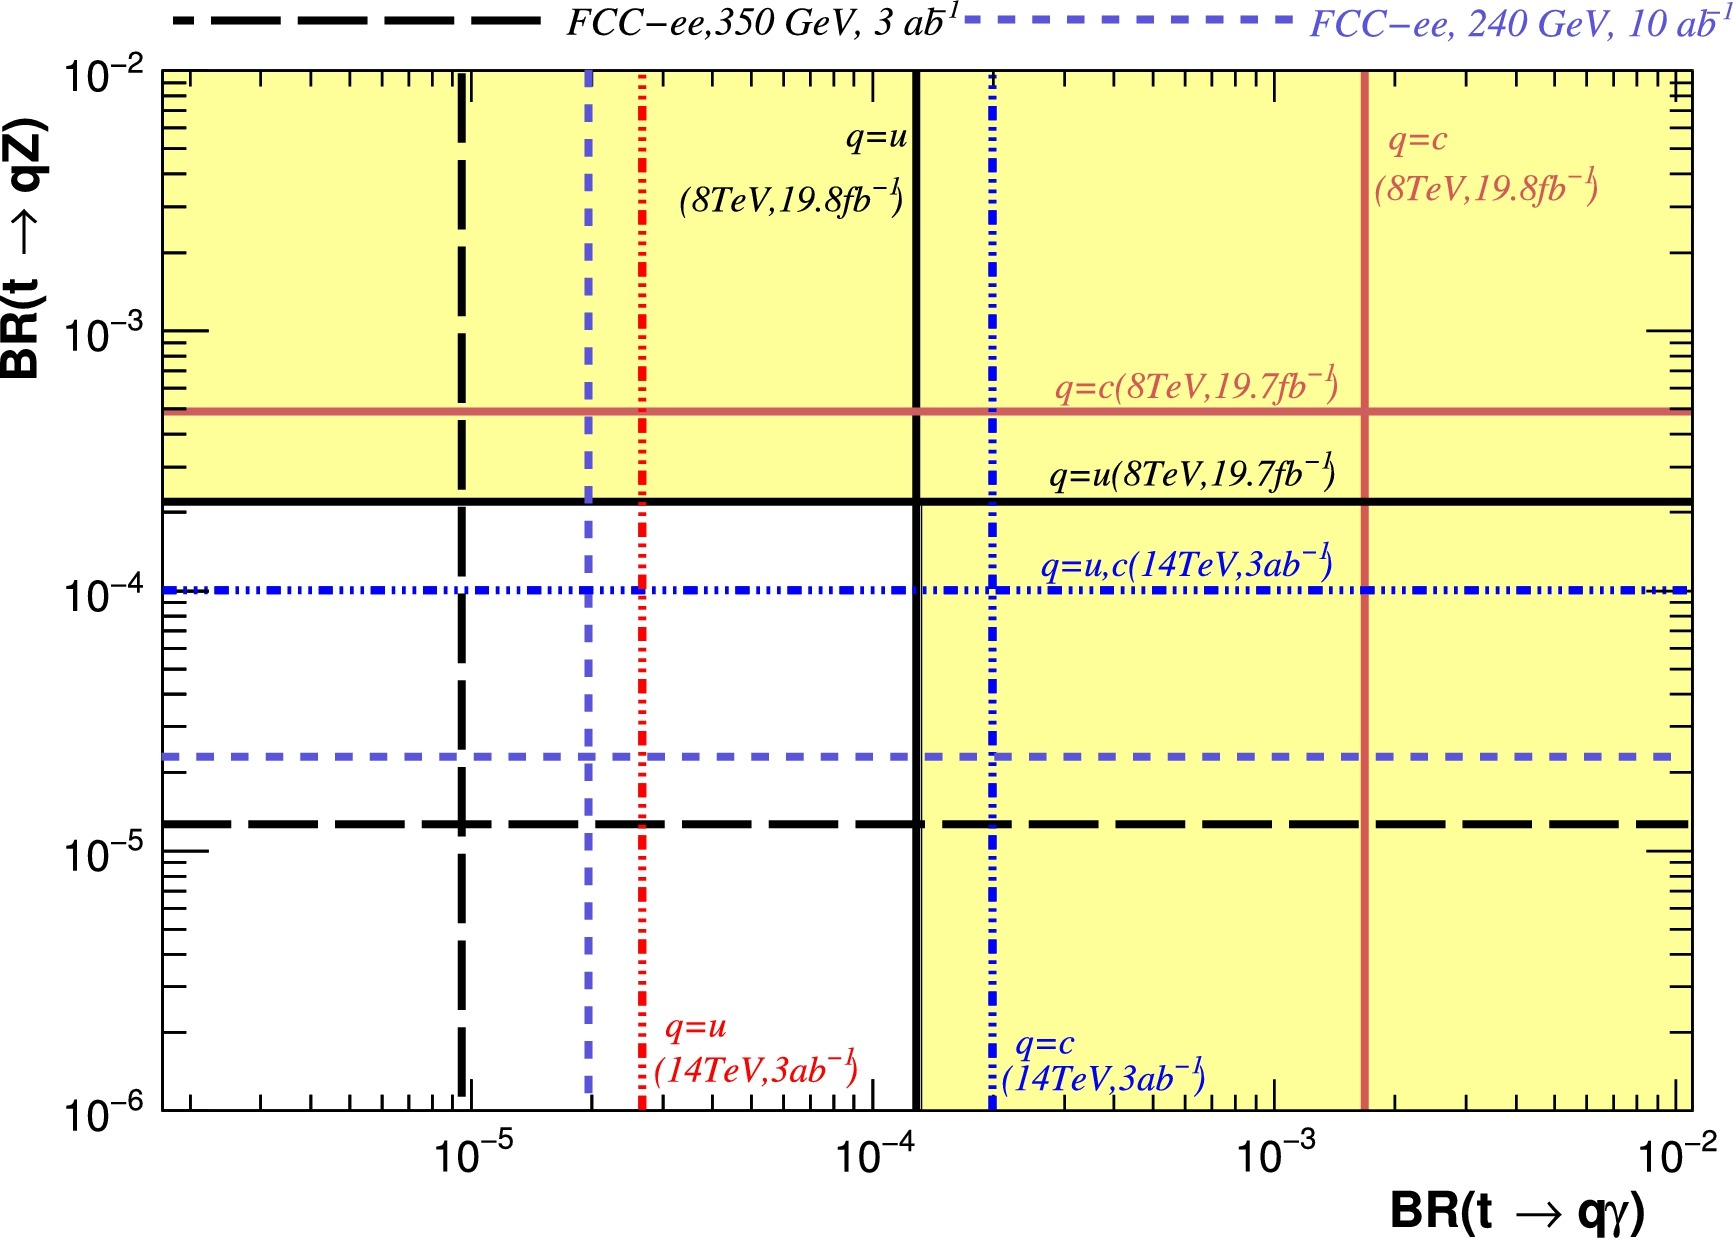
\includegraphics[width=0.49\linewidth]{7_Conclusion/Figures/FCCee}
%	\caption{The observed upper limits on the Br(t → qZ) versus Br(t → qγ) at 95% C.L from the recent analyses of the CMS experiment [13,27]. The expected sensitivity from the CMS experiment with 3000 fb−1 is also shown [30]. The sensitivity of the FCC-ee with 3 ab−1 at the center-of-mass energy of 350 GeV, and with 10 ab−1 at the center-of-mass energy of 240 GeV are presented as well. For the FCC-ee case, at a time one coupling is considered.}
%	\label{fig:fccee}
%\end{figure}

\section{Reflection on the considered EFT model}
%https://indico.cern.ch/event/537012/timetable/#day-2016-11-23
%https://indico.cern.ch/event/643677/contributions/2612456/attachments/1468430/2271112/agrohsje_intro_eft.pdf
There are a few assumptions made in the theoretical model behind this analysis. The lagrangian presented in \eq{eq:EFTlagrangianf}, only considers terms of dimension six. Hence there is no interference with the Standard Model which is of dimension four. However, there can be interference within the FCNC itself. For the \tZq\ couplings, there is a relation with the $\Ptop\Pphoton\Pquark$ through their six-dimensional couplings: 
\begin{equation}
\begin{array}{l l}
\kfqt f^{\mathrm{L}}_{\Pphoton\Pquark} = \frac{v}{g' \Lambda}
\left[\cw \bar{c}_{ uB} - \sw \bar{c}_{ uW}\right]_{i3}^\ast\ ,
\ \   &
\kfqt f^{\mathrm{R}}_{\Pphoton\Pquark} \!=\! \frac{v}{g' \Lambda}
\left[\sw \bar{c}_{ uB} - \cw \bar{c}_{ uW}\right]_{3i} \ ,\\
%
\kZqt f^{\mathrm{L}}_{\PZ\Pquark} = -\frac{2 \cw v}{g \Lambda}
\left[\sw \bar{c}_{ uB} + \cw \bar{c}_{ uW}\right]_{i3}^\ast\ ,
\ \   &
\kZqt f^{\mathrm{R}}_{\PZ\Pquark} \!=\! -\frac{2 \cw v}{g \Lambda}
\left[\cw \bar{c}_{ uB} \!+\! \sw \bar{c}_{ uW}\right]_{3i} \ ,\\
%
\zZqt \tilde f^{\mathrm{L}}_{\PZ\Pquark} = - \frac{2 v^2}{\Lambda^2}
\left[\big(\bar{c}_{ hq}^{(1)}\!-\!\bar{c}_{ hq}^{(3)}\big)_{i3} \!+\!
\big(\bar{c}_{ hq}^{(1)}\!-\!\bar{c}_{ hq}^{(3)}\big)_{3i}^\ast\right]\ ,
\ &
\zZqt \tilde f^{\mathrm{R}}_{\PZ\Pquark} \!=\! - \frac{2 v^2}{\Lambda^2}
\left[(\bar{c}_{ hu})_{i3} + (\bar{c}_{ hu})_{3i}^\ast\right] \ ,\\
\end{array}
\end{equation}
At leading order, both couplings are independent and can be combined to reconstruct the six dimensional operators from the process $\Pproton \Pproton \rightarrow \Ptop\Plepton\APlepton$. The two contributing Feynmann diagrams are shown in \fig{fig:FM}.
\begin{figure}[htbp]
	\centering
	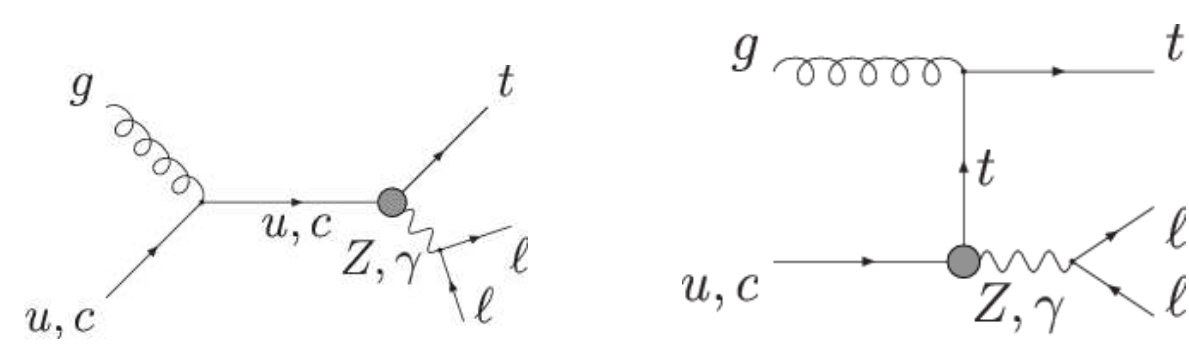
\includegraphics[width=0.7\linewidth]{7_Conclusion/Figures/FM}
	\caption{Leading order Feynmann diagrams contributing to $\Pproton \Pproton \rightarrow \Ptop\Plepton\APlepton$, for the \tZq\ and $\Ptop\Pphoton\Pquark$  anomalous couplings.  }
	\label{fig:FM}
\end{figure}

Another coupling mixing with the \tZq\ coupling, is the $\Ptop\Pgluon\Pquark$ coupling, as can be seen in \fig{fig:FM2}. This coupling could be contributing to the final state considered in the presented analysis.
\begin{figure}[htbp]
	\centering
	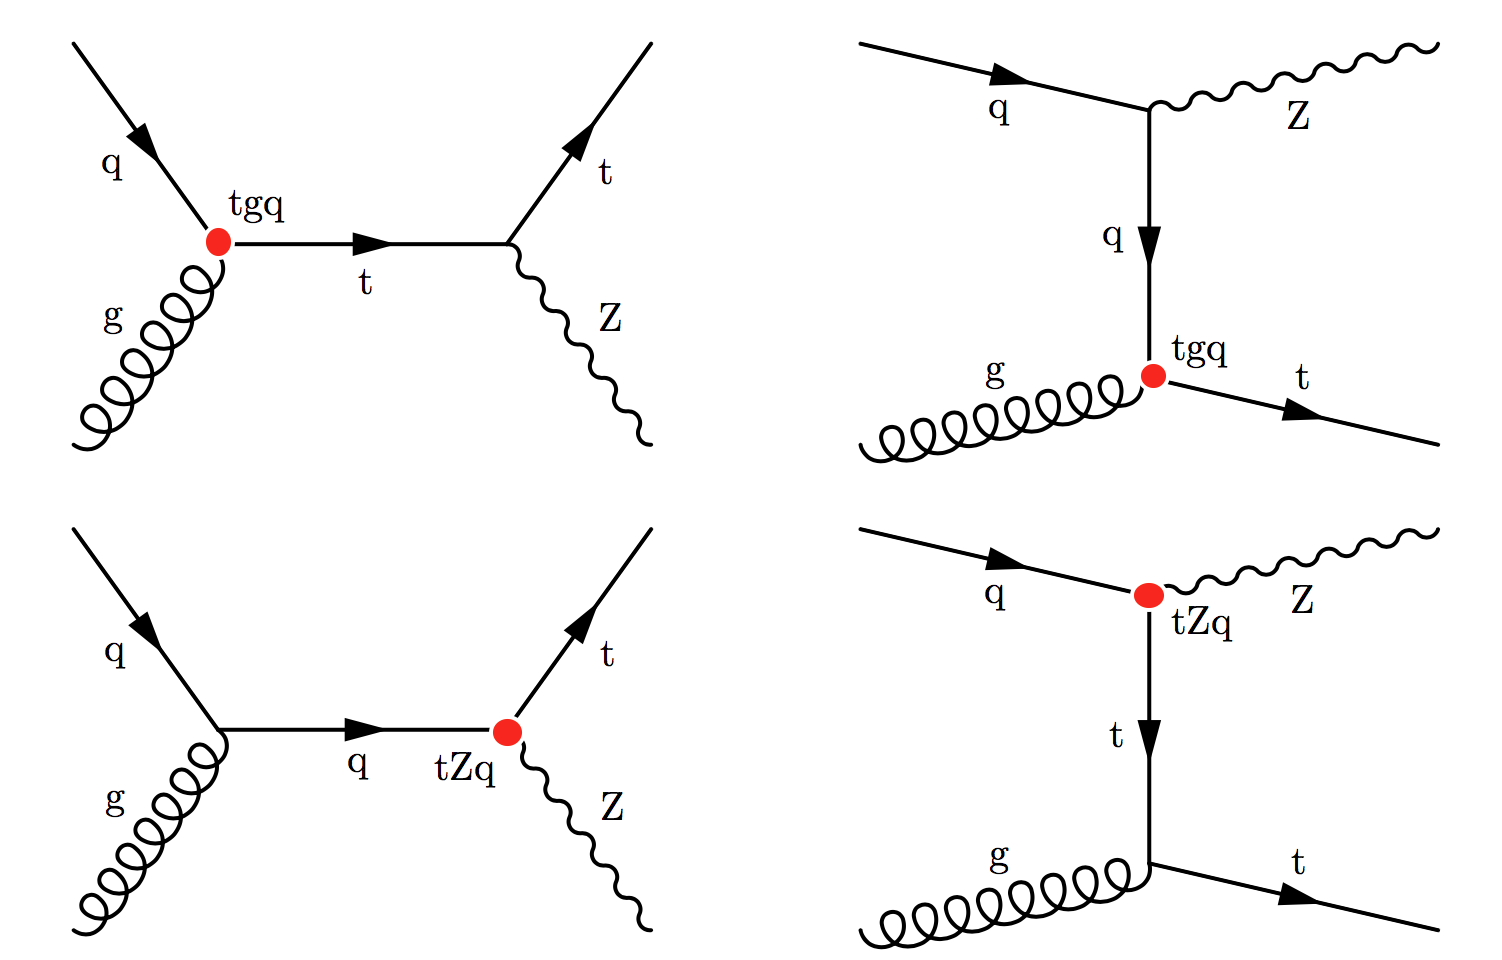
\includegraphics[width=0.7\linewidth]{7_Conclusion/Figures/FM2}
	\caption{Leading order Feynmann diagrams contributing to $\Pproton \Pproton \rightarrow \Ptop\PZ$, for the \tZq\ and $\Ptop\Pgluon\Pquark$  anomalous couplings indicated with a red dot. Figure taken from~\cite{Sirunyan:2017kkr}. }
	\label{fig:FM2}
\end{figure}
However, this coupling would be firstly visible in the top alone final state, before having a visible effect on the final states where it mixes with the other anomalous couplings. Hence, if a FCNC signal is observed in a final state, while no FCNC signal is observed in the top-alone final state, the contribution of the $\Ptop\Pgluon\Pquark$ coupling should be negligible. 

Furthermore, only the Z boson has been considered in the final state. However, new bosons would also candidates giving rise to the same final state. When these new bosons are heavy, their interactions can be contracted and give rise to four-fermion operators which are not considered for the search presented in this thesis. These four-fermion operators involve one top-quark field, one light-quark field, and two leptons~\cite{Zhang:2014ona}, as illustrated in \fig{fig:FM3}.
\begin{figure}[htbp]
	\centering
	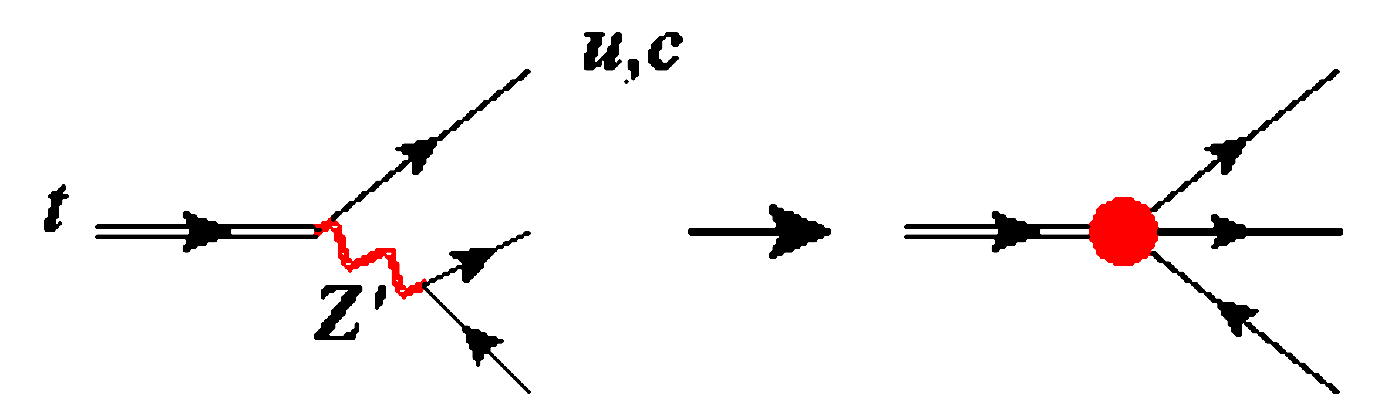
\includegraphics[width=0.5\linewidth]{7_Conclusion/Figures/FM3}
	\caption{Four fermion operators can contribute to $\Ptop \rightarrow \Pquark \Plepton\APlepton$. Figure taken from~\cite{Zhang:2014ona}. }
	\label{fig:FM3}
\end{figure}
 For the $\Pproton \Pproton \rightarrow \Ptop \Plepton\APlepton$ there  is a small contamination of the contributions of four fermion operators at the Z peak that becomes dominant outside the Z peak. This effect is presented in Ref.~\cite{Zhang:2014ona}. For the analysis presented in this thesis, this small contamination is not considered.
 
All of the previous considerations lead to the believe that search for flavour changing neutral currents should evolve towards global analyses for new physics effects. Here, all couplings would be fitted simultaneously in one all-comprehensive global fit. The phenomenology community has already provided first results~\cite{Durieux:2014xla,Buckley:2015lku}, but the correlations between the different experimental inputs get lost  in translation. Recently at CMS, a new top quark EFT analysis group has been founded. With this group a framework is being built to reinterpret the obtained results and global assumptions and operators are used throughout all FCNC searches. 


On top of these considerations, it should also be noted that for the search presented in this analysis, the contribution of the $\zeta_{\Ptop\PZ\Pq}$ coupling is neglected. In Ref.~\cite{Agram:2013koa}, it is shown that this coupling would yield smaller cross sections compared to the \kZqt\ coupling. Therefore, if one would observe the FCNC \tZq\ coupling, this would be more likely coming from the \kZqt\ vertex. Another assumption made from a computational point of view, with the interference between the single top quark FCNC signal and the top quark pair FCNC signal not being considered. This interference would result in an increase of the expected cross section with respect to the one used in this analysis. Hence, the analysis presented in this thesis is setting a more conservative limit on the FCNC anomalous coupling. 
% zeta coupling kane worden genegeerd want kleine cross secties zie https://arxiv.org/pdf/1304.5551.pdf


